\documentclass[onecolumn]{book}
\usepackage{lmodern}
\usepackage{amssymb,amsmath}
\usepackage{ifxetex,ifluatex}
\usepackage{fixltx2e} % provides \textsubscript
\ifnum 0\ifxetex 1\fi\ifluatex 1\fi=0 % if pdftex
  \usepackage[T1]{fontenc}
  \usepackage[utf8]{inputenc}
\else % if luatex or xelatex
  \ifxetex
    \usepackage{mathspec}
  \else
    \usepackage{fontspec}
  \fi
  \defaultfontfeatures{Ligatures=TeX,Scale=MatchLowercase}
\fi
% use upquote if available, for straight quotes in verbatim environments
\IfFileExists{upquote.sty}{\usepackage{upquote}}{}
% use microtype if available
\IfFileExists{microtype.sty}{%
\usepackage{microtype}
\UseMicrotypeSet[protrusion]{basicmath} % disable protrusion for tt fonts
}{}
\usepackage[margin=1in]{geometry}
\usepackage{hyperref}
\hypersetup{unicode=true,
            pdftitle={Compositional analysis of high throughput sequencing data},
            pdfauthor={Greg Gloor},
            pdfborder={0 0 0},
            breaklinks=true}
\urlstyle{same}  % don't use monospace font for urls
\usepackage{color}
\usepackage{fancyvrb}
\newcommand{\VerbBar}{|}
\newcommand{\VERB}{\Verb[commandchars=\\\{\}]}
\DefineVerbatimEnvironment{Highlighting}{Verbatim}{commandchars=\\\{\}}
% Add ',fontsize=\small' for more characters per line
\usepackage{framed}
\definecolor{shadecolor}{RGB}{248,248,248}
\newenvironment{Shaded}{\begin{snugshade}}{\end{snugshade}}
\newcommand{\AlertTok}[1]{\textcolor[rgb]{0.94,0.16,0.16}{#1}}
\newcommand{\AnnotationTok}[1]{\textcolor[rgb]{0.56,0.35,0.01}{\textbf{\textit{#1}}}}
\newcommand{\AttributeTok}[1]{\textcolor[rgb]{0.77,0.63,0.00}{#1}}
\newcommand{\BaseNTok}[1]{\textcolor[rgb]{0.00,0.00,0.81}{#1}}
\newcommand{\BuiltInTok}[1]{#1}
\newcommand{\CharTok}[1]{\textcolor[rgb]{0.31,0.60,0.02}{#1}}
\newcommand{\CommentTok}[1]{\textcolor[rgb]{0.56,0.35,0.01}{\textit{#1}}}
\newcommand{\CommentVarTok}[1]{\textcolor[rgb]{0.56,0.35,0.01}{\textbf{\textit{#1}}}}
\newcommand{\ConstantTok}[1]{\textcolor[rgb]{0.00,0.00,0.00}{#1}}
\newcommand{\ControlFlowTok}[1]{\textcolor[rgb]{0.13,0.29,0.53}{\textbf{#1}}}
\newcommand{\DataTypeTok}[1]{\textcolor[rgb]{0.13,0.29,0.53}{#1}}
\newcommand{\DecValTok}[1]{\textcolor[rgb]{0.00,0.00,0.81}{#1}}
\newcommand{\DocumentationTok}[1]{\textcolor[rgb]{0.56,0.35,0.01}{\textbf{\textit{#1}}}}
\newcommand{\ErrorTok}[1]{\textcolor[rgb]{0.64,0.00,0.00}{\textbf{#1}}}
\newcommand{\ExtensionTok}[1]{#1}
\newcommand{\FloatTok}[1]{\textcolor[rgb]{0.00,0.00,0.81}{#1}}
\newcommand{\FunctionTok}[1]{\textcolor[rgb]{0.00,0.00,0.00}{#1}}
\newcommand{\ImportTok}[1]{#1}
\newcommand{\InformationTok}[1]{\textcolor[rgb]{0.56,0.35,0.01}{\textbf{\textit{#1}}}}
\newcommand{\KeywordTok}[1]{\textcolor[rgb]{0.13,0.29,0.53}{\textbf{#1}}}
\newcommand{\NormalTok}[1]{#1}
\newcommand{\OperatorTok}[1]{\textcolor[rgb]{0.81,0.36,0.00}{\textbf{#1}}}
\newcommand{\OtherTok}[1]{\textcolor[rgb]{0.56,0.35,0.01}{#1}}
\newcommand{\PreprocessorTok}[1]{\textcolor[rgb]{0.56,0.35,0.01}{\textit{#1}}}
\newcommand{\RegionMarkerTok}[1]{#1}
\newcommand{\SpecialCharTok}[1]{\textcolor[rgb]{0.00,0.00,0.00}{#1}}
\newcommand{\SpecialStringTok}[1]{\textcolor[rgb]{0.31,0.60,0.02}{#1}}
\newcommand{\StringTok}[1]{\textcolor[rgb]{0.31,0.60,0.02}{#1}}
\newcommand{\VariableTok}[1]{\textcolor[rgb]{0.00,0.00,0.00}{#1}}
\newcommand{\VerbatimStringTok}[1]{\textcolor[rgb]{0.31,0.60,0.02}{#1}}
\newcommand{\WarningTok}[1]{\textcolor[rgb]{0.56,0.35,0.01}{\textbf{\textit{#1}}}}
\usepackage{longtable,booktabs}
\usepackage{graphicx,grffile}
\makeatletter
\def\maxwidth{\ifdim\Gin@nat@width>\linewidth\linewidth\else\Gin@nat@width\fi}
\def\maxheight{\ifdim\Gin@nat@height>\textheight\textheight\else\Gin@nat@height\fi}
\makeatother
% Scale images if necessary, so that they will not overflow the page
% margins by default, and it is still possible to overwrite the defaults
% using explicit options in \includegraphics[width, height, ...]{}
\setkeys{Gin}{width=\maxwidth,height=\maxheight,keepaspectratio}
\IfFileExists{parskip.sty}{%
\usepackage{parskip}
}{% else
\setlength{\parindent}{0pt}
\setlength{\parskip}{6pt plus 2pt minus 1pt}
}
\setlength{\emergencystretch}{3em}  % prevent overfull lines
\providecommand{\tightlist}{%
  \setlength{\itemsep}{0pt}\setlength{\parskip}{0pt}}
\setcounter{secnumdepth}{0}
% Redefines (sub)paragraphs to behave more like sections
\ifx\paragraph\undefined\else
\let\oldparagraph\paragraph
\renewcommand{\paragraph}[1]{\oldparagraph{#1}\mbox{}}
\fi
\ifx\subparagraph\undefined\else
\let\oldsubparagraph\subparagraph
\renewcommand{\subparagraph}[1]{\oldsubparagraph{#1}\mbox{}}
\fi

%%% Use protect on footnotes to avoid problems with footnotes in titles
\let\rmarkdownfootnote\footnote%
\def\footnote{\protect\rmarkdownfootnote}

%%% Change title format to be more compact
\usepackage{titling}

% Create subtitle command for use in maketitle
\newcommand{\subtitle}[1]{
  \posttitle{
    \begin{center}\large#1\end{center}
    }
}

\setlength{\droptitle}{-2em}
  \title{Compositional analysis of high throughput sequencing data}
  \pretitle{\vspace{\droptitle}\centering\huge}
  \posttitle{\par}
  \author{Greg Gloor}
  \preauthor{\centering\large\emph}
  \postauthor{\par}
  \predate{\centering\large\emph}
  \postdate{\par}
  \date{03 April, 2018}

\usepackage{geometry}
\usepackage{amsmath}
\newcommand{\ith}[1]{ #1\textsuperscript{th}\ }
\newcommand{\vect}[1]{\vec{\textbf{#1}}}
\setlength{\columnsep}{18pt} 

\setlength\textwidth{5.5in}
\setlength\marginparwidth{1.5in}

\usepackage{amsthm}
\newtheorem{theorem}{Theorem}
\newtheorem{lemma}{Lemma}
\theoremstyle{definition}
\newtheorem{definition}{Definition}
\newtheorem{corollary}{Corollary}
\newtheorem{proposition}{Proposition}
\theoremstyle{definition}
\newtheorem{example}{Example}
\theoremstyle{definition}
\newtheorem{exercise}{Exercise}
\theoremstyle{remark}
\newtheorem*{remark}{Remark}
\newtheorem*{solution}{Solution}
\begin{document}
\maketitle

{
\setcounter{tocdepth}{2}
\tableofcontents
}
\hypertarget{about}{%
\chapter{About this document}\label{about}}

This document is an .Rmd document and can be found at:

github.com/ggloor/book

The generation of this document requires \texttt{R} and an installation
of \LaTeX to work properly. This document contains interspersed markdown
and \texttt{R} code that may be compiled into a pdf document and
supports the figures and assertions in the main article. \texttt{R} code
is (almost always) exposed in the pdf document so that the interested
reader can work through the example code themselves. Code that is not
exposed is in the \texttt{chunk} directory.

\hypertarget{reproducing-the-analysis}{%
\section{Reproducing the analysis}\label{reproducing-the-analysis}}

From an R command prompt you can compile this document into PDF if you
have \LaTeX and pandoc installed:

\texttt{bookdown::render\_book("index.Rmd")} or you can open the file in
RStudio and compile in that environment.

\hypertarget{r-packages-required}{%
\section{R packages required}\label{r-packages-required}}

We will need the following R packages, several functions are defined in
a dedicated functions section.

\begin{enumerate}
\def\labelenumi{\arabic{enumi}.}
\tightlist
\item
  knitr (CRAN)
\item
  bookdown (CRAN)
\item
  vegan (CRAN)
\end{enumerate}

\hypertarget{intro}{%
\chapter{Introduction}\label{intro}}

\hspace{2cm}\begin{minipage}[ct]{10cm}
\parskip=5pt
\parindent=5pt

"What really is the point of trying to teach anything to anybody?"

This question seemed to provoke a murmur of sympathetic approval from up and down the table.

 Richard continued, "What I mean is that if you really want to understand something, the best way is to try and explain it to someone else. That forces you to sort it out in your mind. And the more slow and dim-witted your pupil, the more you have to break things down into more and more simple ideas. And that's really the essence of programming. By the time you've sorted out a complicated idea into little steps that even a stupid machine can deal with, you've learned something about it yourself. The teacher usually learns more than the pupils. Isn't that true?" [Richard MacDuff] \footnote{Douglas Adams, 1987 in \emph{Dirk Gently's Holistic Detection Agency},  William Heinemann Ltd, London}

 \vspace{1cm}
 Let us think the unthinkable, let us do the undoable, let us prepare to grapple with the ineffable itself, and see if we may not eff it after all. [Dirk Gently] \footnote{ibid}

\end{minipage}

This booklet is intended for use in teaching graduate student courses
and conference workshops on using compositional data analysis methods to
examine high throughput sequencing datasets. The approach taken here is
largely intuitive and hands on. Formulas for basic methodologies are
presented, but the intuitive reason for using them takes precedence. The
methods presented here have been used for 16S rRNA gene sequencing,
transcriptomics, metagenomics and in-vitro selection (selex)
experiments.

The first section is background and theory using toy examples. The
second section is application of what we have learned using practical
examples. I hope you find this useful.

\hypertarget{outline-of-the-material}{%
\section{Outline of the material}\label{outline-of-the-material}}

\begin{itemize}
\tightlist
\item
  I begin with a brief overview of sequencing technologies, an overview
  of the types of data we are likely to encounter, and describe how and
  why these instruments generate data that are constrained to a constant
  count.
\item
  I introduce sequencing as a stochastic process, explain why we need to
  estimate our technical variance and show how this can be done
  technical variance
\item
  I next semi-formally introduce compositional data, and show with
  examples the pathologies associated with this type of data.
\item
  I then introduce common data transforms and distances used in the high
  throughput sequencing literature, and demonstrate that none of the
  transforms affects the compositional nature of the data, and that in
  fact, many of the transforms affect the data in non-intuitive ways
\item
  I begin the practical part with exploratory data analysis using the
  compositional biplot
\item
  I describe the properties of three types of plots to examine high
  dimensional data: Bland-Altman plots (MA plots), volcano plots, and
  effect plots
\item
  I describe compositionally appropriate methods to estimate
  differential abundance with an emphasis on ALDEx2 and to a lesser
  extent ANCOM
\item
  I describe compositional association as a replacement for correlation
  using the propr R package
\end{itemize}

\hypertarget{sequencing}{%
\chapter{The nature of sequencing data}\label{sequencing}}

There are a tremendous number of high throughput sequence analysis tools
in the literature. The vast majority of these are recommended for use in
only one domain. Domain specific tools are found in all experimental
designs and are often touted as `optimized for' a particular design.
Another, less charitable way of describing a domain-specific tool is
`over-parameterized'. It is important to make as few assumptions as
possible when examining data, and to ensure that the data being analyzed
and the assumptions of the analysis tools are met (Box
\protect\hyperlink{ref-box:1976}{1976}).

\hspace{2cm}\begin{minipage}[ct]{10cm}
\parskip=5pt
\parindent=5pt

Since all models are wrong the scientist cannot obtain a "correct" one by excessive elaboration. On the contrary following William of Occam he should seek an economical description of natural phenomena. Just as the ability to devise simple but evocative models is the signature of the great scientist so overelaboration and overparameterization is often the mark of mediocrity.\footnote{George Box 1976 \emph{Science and Statistics}. J. Am. Stat. Soc. 71:791}

\end{minipage}

\hypertarget{a-constrained-random-sample}{%
\section{A constrained random
sample}\label{a-constrained-random-sample}}

All high throughput gene sequencing datasets share a common origin and
it is important to understand the source of the data, and the standard
workflow. In essence, an arbitrarily large population of DNA molecules
is randomly sampled from an environment and a small, fixed number of
those molecules are sequenced.

There is a frequent assertion that data generated by high throughput
sequencing instruments are counts. On the surface, this makes sense
because we map reads to intervals and we observe the number of counts
per interval. However, immediately problems arise. One pervasive issue
is that the results are strongly influenced by the total read count per
sample, and this is the primary reason for almost all tools using `count
normalization' methods that are introduced later.

The `un-constrained Random Sample' panel in Figure 3.1 shows how random
sampling is usually thought of. We start with an imaginary population
containing four different randomly distributed entities, tigers,
ladybugs, aliens and rabbits. We want to infer the abundance of each
entity in the population by taking a random sample. This is done by
choosing a particular area (or volume) to sample and counting the number
of each entity in the area. Doing this, we observe 14 rabbits, 1 alien,
24 ladybugs and 6 tigers. We can use this random sample to infer
something about the abundances of the entities in the population.

\begin{figure}
\centering
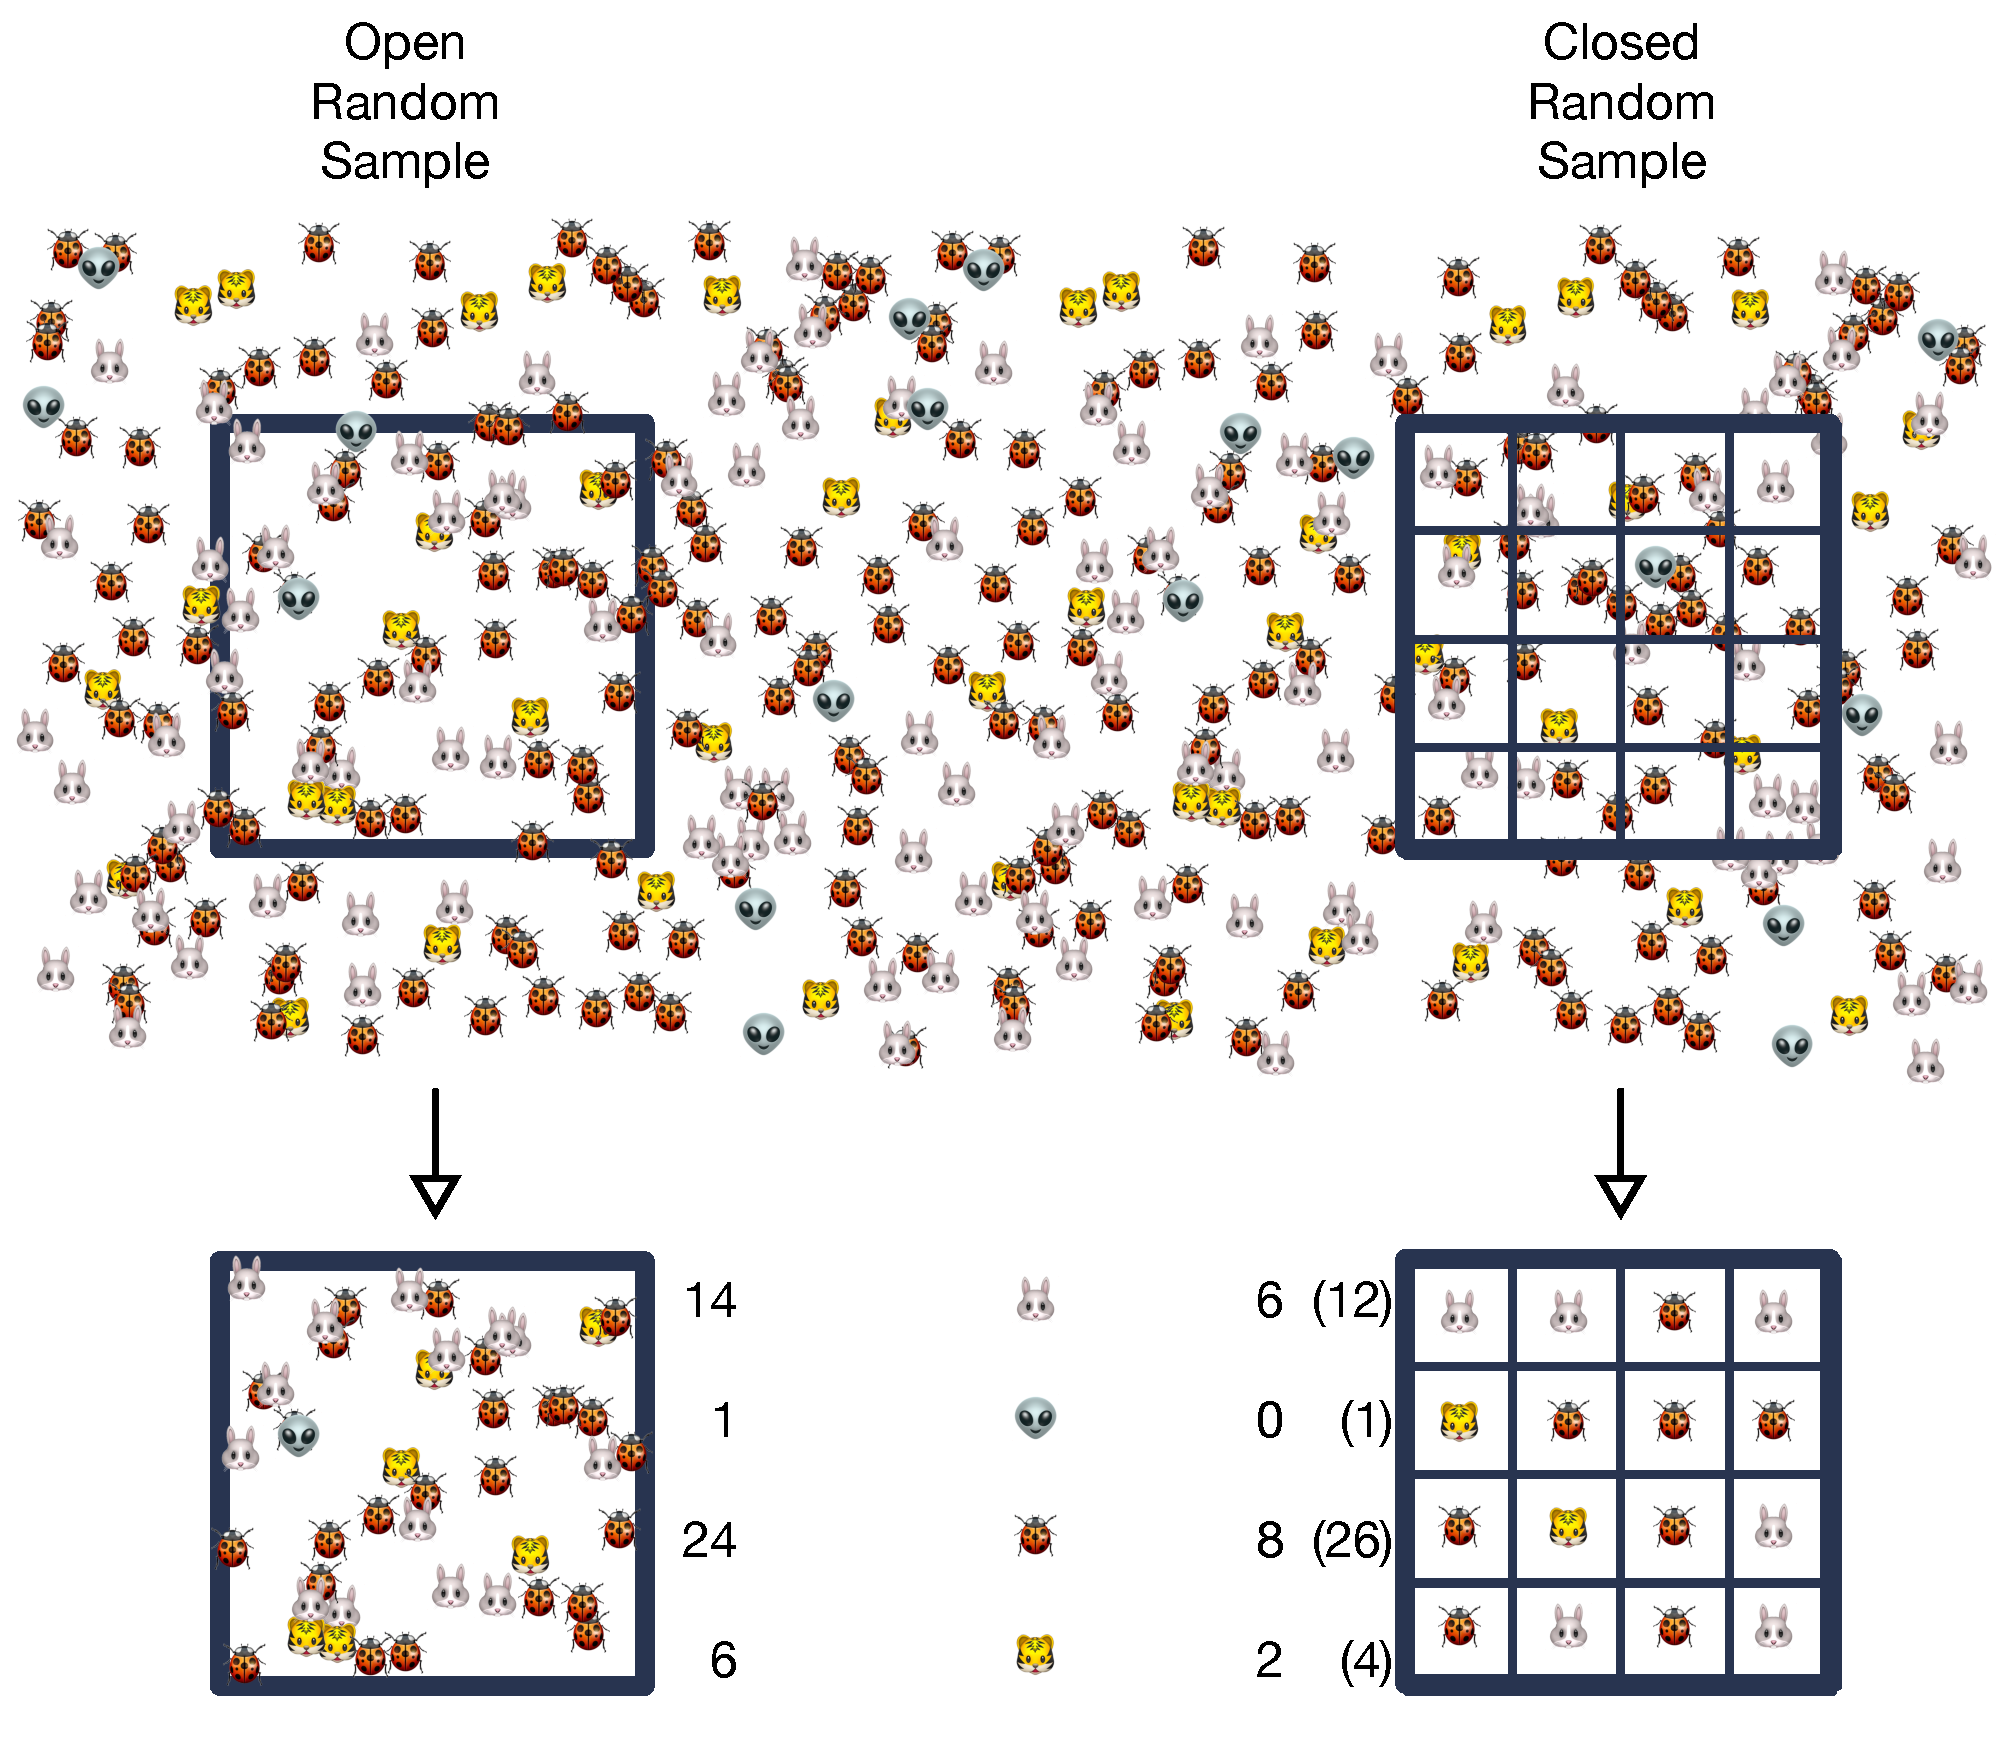
\includegraphics{figs/RALT.pdf}
\caption{\label{RALT} DNA sequencing is a defined-limit random sample of
the environment. We start with a population of four entities randomly
distributed; rabbits, aliens, ladybugs and tigers. The standard approach
to randomly sample a fixed area of the field. This is an `un-constrained
random sample' since the \emph{number} of entities found inside the
sampling area is a direct readout of the sampled area. In contrast, DNA
sequencing is constrained by the number of fragments that the machine
can accomodate. This is akin to filling the squares on a checker board,
where only one entity is allowed per square. This is shown in the
`constrained random sample' box.}
\end{figure}

A single random sample will of course limit the precision of estimation
of the population characteristics. The reason that we replicate
experimental measurements is to estimate and to place limits on the
precision of the estimates of population parameters. A second random
sample is shown on the right and is labeled as a `constrained random
sample' (the constraint will be explained shortly). The second random
sample, with the same area contains 12 rabbits, one alien, 26 ladybugs
and 4 tigers. The first estimate had a total of 45 entities, and the
second had a total of 43 entities. Two important points need to be made.
First, we are comparing the numbers of each type of entity, and second,
the total number of entities identified in each sample is free to vary.
In theory, we could sample a the same area that is very densely
populated by ladybugs (perhaps it is mating season) and identify
thousands of ladybugs in a very small area.

DNA sequencing is not a counting exercise because the total number of
entities found is constrained by the capacity of the instrument. Imagine
the worlds worst high throughput sequencer, the GS16™ (GregSeq16™). The
GS16 has a total capacity of 16 molecules, any more and it fails, any
fewer and the customer is upset because they did not receive the number
of reads promised by the very slick sales brochure. The process of
filling the 16 slots proceeds by a random process whereby the first
entity to occupy a slot is sequenced, and any subsequent entities are
unable to bind to the proprietary surface. As outlined later this is
akin to the processes involved in all current high throughput sequencing
instruments. Applying this random process to the entities in the second
sample, we observe that the GS16™ delivers 6 rabbits, 0 aliens, 8
ladybugs and 4 tigers. In the event that we sample from the area where
the ladybugs were mating, we would recognize only that there were 16
ladybugs in the area, and miss entirely that the area was a seething
mass of ladybugs: that is, we would be unable to distinguish if the
sample just happened to be from a site that was missing the other
entities, or from a site that contained a vast number of ladybugs.

\hypertarget{constrained-and-un-constrained-environments.}{%
\section{Constrained and un-constrained
environments.}\label{constrained-and-un-constrained-environments.}}

There are two types of environments. In the un-constrained environment
the total number of entities in the environment is free to change. A
constrained environment, in contrast is operating at some pre-determined
limit or carrying capacity.

In Figure \ref{RALT} we were modelling what happens when the environment
is un-constrained, that is, the environment can contain arbitrarily
greater or fewer numbers of any entity. Two real-world examples spring
to mind of such an un-constrained environment. The first example would
be the consortium of organisms that inhabit the human vagina and which
occur in at least two major states. The first state is dominated by one
or a small number of species from the genus \emph{Lactobacillus}. The
second state is dominated by a mixed population of anaerobic species.
The total numbers of bacteria (bacterial load) in the second state is
about 100-fold greater than in the second state (Zozaya-Hinchliffe et
al. \protect\hyperlink{ref-Zozaya:2010}{2010}). When comparing either
DNA or RNA molecules from these two populations we would need to ensure
that we account for the un-constrained nature of the system and not
assume that the total number of molecules sampled is equivalent. The
second example of an un-constrained environment would be in-vitro
selection experiments as published in (McMurrough et al.
\protect\hyperlink{ref-mcmurrough:2014}{2014}; Wolfs et al.
\protect\hyperlink{ref-Wolfs:2016aa}{2016}) where there are two
different classes of genes; inactive genes where the absolute abundance
of the corresponding DNA molecules remains unchanged over time, and
active genes where the absolute abundance of the corresponding DNA
molecules increases exponentially. In both these types of experiment,
the absolute number of molecules is free to change.

A constrained environment arises when the underlying system is operating
at some fixed limit. As an example, a culture of
\emph{Escherichia coli}, a common lab strain of bacteria, that is
growing in the lab under controlled conditions has a near constant
number of RNA molecules in each cell (Bernstein et al.
\protect\hyperlink{ref-mRNA:2002}{2002}). Moreover, when a new gene is
induced to make new mRNA molecules under these standard conditions the
number of RNA molecules of very highly expressed genes is reduced to
compensate (Taniguchi et al.
\protect\hyperlink{ref-Taniguchi:2010aa}{2010}). Thus, under a given
condition, the total number of mRNA molecules in a cell has a fixed
limit: the cell cannot exceed this limit under the given condition. In
this case all mRNA molecules in the system are inherently coupled, a
change in absolute abundance of one molecule is compensated for by a
change in absolute abundance by one or more others to ensure that the
total number of molecules in the system is relatively constant. In the
language of sports analogies ``a single cell cannot give 110\% effort''.
It is assumed that mRNA molecular abundance in most lab cultures of most
cell types behave similarly.

Obviously many real datasets exist on a continuum between these example
extremes, but it is not always obvious at which extreme a given sample
lay. For example, when comparing gene expression in liver and kidney
cells do we expect the same number of underlying molecules per cell?
What about comparing liver and red blood cells? Here the choice is more
obvious since the red blood cells are much less metabolically active and
express far fewer unique mRNA molecules than does the typical liver
cell. Knowing if the samples are from a constrained or un-constrained
system has important implications for analysis as outlined below. As we
shall see in the practical examples, most tools work acceptably well
with constrained data, but fail in unexpected ways on un-constrained
data.

\hypertarget{modeling-constrained-and-un-constrained-samples}{%
\section{Modeling constrained and un-constrained
samples}\label{modeling-constrained-and-un-constrained-samples}}

A simple thought experiment should clarify the importance of knowing the
difference between constrained and un-constrained systems. In this
example I generate a test dataset composed of 100 features in 20
samples---modelled as a time series with 20 steps. There are two
situations. In the `constrained' situation, one feature increase
exponentially in each time step and one other feature decreases to
compensate . In the `un-constrained' situation, only one feature
increases while the remainder of the features remain at a constant total
abundance.

\begin{Shaded}
\begin{Highlighting}[]
\NormalTok{num.one =}\StringTok{ }\DecValTok{90} \CommentTok{# base number of features}

\NormalTok{m.dub <-}\StringTok{ }\NormalTok{prop.m <-}\StringTok{ }\NormalTok{clr.m <-}\StringTok{ }\NormalTok{m.dub.u <-}\StringTok{ }\NormalTok{prop.m.u <-}\StringTok{ }\NormalTok{clr.m.u <-}
\StringTok{    }\KeywordTok{matrix}\NormalTok{(}\DataTypeTok{data=}\OtherTok{NA}\NormalTok{, }\DataTypeTok{nrow=}\DecValTok{20}\NormalTok{, }\DataTypeTok{ncol=}\NormalTok{num.one }\OperatorTok{+}\StringTok{ }\DecValTok{10}\NormalTok{)}

\NormalTok{in.put <-}\StringTok{ }\KeywordTok{c}\NormalTok{(}\DecValTok{10}\NormalTok{,}\DecValTok{10000}\NormalTok{,}\DecValTok{1}\NormalTok{,}\DecValTok{5}\NormalTok{,}\DecValTok{10}\NormalTok{,}\DecValTok{20}\NormalTok{,}\DecValTok{50}\NormalTok{,}\DecValTok{100}\NormalTok{,}\DecValTok{200}\NormalTok{,}\DecValTok{1000}\NormalTok{) }\CommentTok{# arbitrary data}

\CommentTok{# ensure feature 3 is arbitrarily large and get the constrained total}
\NormalTok{total.sum <-}\StringTok{ }\KeywordTok{sum}\NormalTok{(in.put }\OperatorTok{+}\StringTok{ }\DecValTok{1}\NormalTok{) }\OperatorTok{*}\StringTok{ }\DecValTok{1000}

\CommentTok{# one feature increases exponentially and one feature decreases to compensate}
\ControlFlowTok{for}\NormalTok{(i }\ControlFlowTok{in} \DecValTok{0}\OperatorTok{:}\DecValTok{19}\NormalTok{)\{}
    \CommentTok{# un-constrained data, feature 1 exponentially increases}
\NormalTok{    m.dub[i}\OperatorTok{+}\DecValTok{1}\NormalTok{,] <-}\StringTok{ }\NormalTok{m.dub.u[i}\OperatorTok{+}\DecValTok{1}\NormalTok{,] <-}\StringTok{ }\NormalTok{in.put }\OperatorTok{*}\StringTok{ }\KeywordTok{c}\NormalTok{(}\DecValTok{2}\OperatorTok{^}\NormalTok{i, }\KeywordTok{rep}\NormalTok{(}\DecValTok{1}\NormalTok{,num.one }\OperatorTok{+}\StringTok{ }\DecValTok{9}\NormalTok{))}
\NormalTok{    prop.m.u[i}\OperatorTok{+}\DecValTok{1}\NormalTok{,] <-}\StringTok{ }\NormalTok{m.dub.u[i}\OperatorTok{+}\DecValTok{1}\NormalTok{,]}\OperatorTok{/}\KeywordTok{sum}\NormalTok{(m.dub.u[i}\OperatorTok{+}\DecValTok{1}\NormalTok{,])}
\NormalTok{    clr.m.u[i}\OperatorTok{+}\DecValTok{1}\NormalTok{,] <-}\StringTok{ }\DecValTok{2}\OperatorTok{^}\NormalTok{(}\KeywordTok{log2}\NormalTok{(prop.m.u[i}\OperatorTok{+}\DecValTok{1}\NormalTok{,]) }\OperatorTok{-}\StringTok{ }\KeywordTok{mean}\NormalTok{(}\KeywordTok{log2}\NormalTok{(prop.m.u[i}\OperatorTok{+}\DecValTok{1}\NormalTok{,])))}
    \CommentTok{# now constrain the data, feature 3 decreases to compensate}
\NormalTok{    m.dub[i}\OperatorTok{+}\DecValTok{1}\NormalTok{,}\DecValTok{3}\NormalTok{] <-}\StringTok{ }\NormalTok{total.sum }\OperatorTok{-}\StringTok{ }\KeywordTok{sum}\NormalTok{(m.dub[i}\OperatorTok{+}\DecValTok{1}\NormalTok{,])}
\NormalTok{    prop.m[i}\OperatorTok{+}\DecValTok{1}\NormalTok{,] <-}\StringTok{ }\NormalTok{m.dub[i}\OperatorTok{+}\DecValTok{1}\NormalTok{,] }\OperatorTok{/}\StringTok{ }\KeywordTok{sum}\NormalTok{(m.dub[i}\OperatorTok{+}\DecValTok{1}\NormalTok{,])}
\NormalTok{    clr.m[i}\OperatorTok{+}\DecValTok{1}\NormalTok{,] <-}\StringTok{ }\KeywordTok{log2}\NormalTok{(prop.m[i}\OperatorTok{+}\DecValTok{1}\NormalTok{,]) }\OperatorTok{-}\StringTok{ }\KeywordTok{mean}\NormalTok{(}\KeywordTok{log2}\NormalTok{(prop.m[i}\OperatorTok{+}\DecValTok{1}\NormalTok{,]))}
\NormalTok{\}}
\end{Highlighting}
\end{Shaded}

\begin{figure}

{\centering 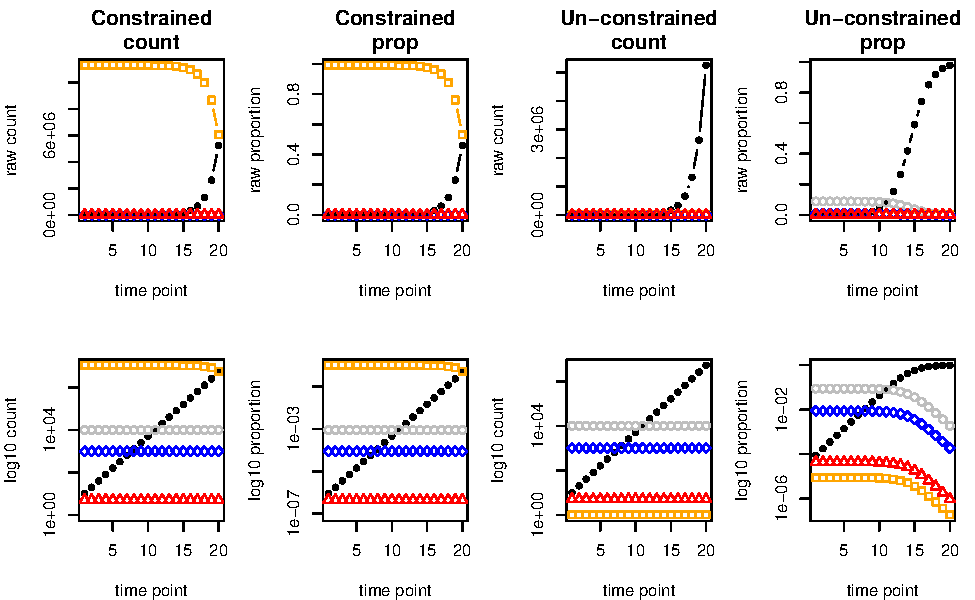
\includegraphics[width=0.9\linewidth]{_main_files/figure-latex/shape-1} 

}

\caption{Constrained and un-constrained data are very different. The 'Constrained count' column shows a synthetic dataset where the total number of counts is a constant and this is plotted as counts on top and on a log10 scale on the bottom. Here we see that the orange and black features are compensating and perfectly negatively correlated. These same data are next converted to proportions or relative abundances and plotted in the 'Constrained prop' column. Both the count and proportional data are the same, except for the scale, when the data are constrained. The un-constrained data behave differently. The 'un-constrained count' and 'un-constrained prop' columns are distinct and the proportional data are severely distorted. The un-constrained counts are all independent, but the  exponentially increasing feature in black is negatively correlated with the constant features in the un-constrained proportion plot. Only 5 of the 100 features are shown for clarity.}\label{fig:shape}
\end{figure}

Of course DNA sequencing is not the same as our synthetic example. When
collecting samples and sequencing them, there are many more features,
and significantly more noise because of random sampling that modelled in
Figure \ref{fig:shape}. There are many sources of sampling error or even
sampling bias. Nevertheless, this example serves as an instructive
starting point.

\hypertarget{instrument-capacity}{%
\subsection{Instrument capacity}\label{instrument-capacity}}

So how is sequencing a constrained operation? Each instrument has its
own specific capacity issues that must be taken into account.

The Ion Torrent and Ion Proton systems have a chip with a predetermined
number of pores on the sequencing chip (10 of thousands to 10s of
millions, depending on the chip) that can accept a library fragment. No
signal is returned from an empty pore, and the signal is rejected if a
pore contains two or more different fragments. Sequencing is successful
only when the pore is occupied by a single fragment from the library.
This is directly analogous to the Constrained Random Sample panel in
Figure \ref{RALT}

The Illumina sequencing instruments attach the DNA fragments to a glass
slide and then each fragment is amplified into millions of identical
fragments called clusters which appear as randomly distributed spots
under a microscope. Each different Illumina instrument accommodates a
characteristic maximum number of clusters, and if two or more clusters
overlap they are rejected by the software. Thus, there is a fixed number
of spots that can be accomodated on the Illumina sequencing chip just as
there are a fixed number of slots on the Ion platforms or the GregSeq.

Thus, regardless of instrument, the technician must apply a precise
number of DNA molecules that maximizes the number of fragments on the
sequencing instrument without overloading it. It should be obvious that
loading a DNA sequencer is akin to filling the squares on a checkerboard
where the goal is to have as many checkers as possible, without
overlapping the pieces. DNA sequencing instruments have an upper bound
on the number of fragments they can sequence, and as we shall see later,
any arbitrary upper bound is equivalent to a proportion. This means that
high-throughput sequencing affects the shape of the data differently on
constrained and un-constrained data as shown on Figure \ref{fig:shape}.

We assume that the abundance of each input DNA species that is observed
after sequencing reflects in some linear way a random sample of the
input molecules. This is likely to be the case if the total number of
molecules in the input sample is constrained. Such a constraint would be
met if, for example, an increase in one or more DNA species was balanced
with an equivalent decrease in one or more different species. However,
as we shall see, the analysis of un-constrained data will be a problem
if the limited output of the sequencing platform is not accounted for.

\hypertarget{example-calculation-of-fragment-number}{%
\subsection{Example calculation of fragment
number}\label{example-calculation-of-fragment-number}}

The number of fragments after sequencing is determined by the
instrument; an Ilumina MiSeq delivers \(\sim 20\)M fragments whereas an
Illumina NextSeq delivers \(\sim 400\)M and an Illumina HiSeq can
deliver \(\sim 250\)M reads per lane on each of 8 lanes. The commonly
used Nextera DNA library kit is optimized to require 50 ng of DNA per
sample. Thus, the number of fragments of DNA (or RNA) molecules in the
underlying environment, in general, vastly outnumbers the number of
sequence fragments from which the library is made, and the number of
fragments in the library in turn outnumbers the number of fragments from
which sequencing data are ultimately derived. We can do a simple back of
the envelope calculation for an example metagenomics sequencing run to
show this.

Assume that we have a mixture of bacterial species with a mean genome
size of 4 Mb. One mole of genomes would have a mass of
\(2.64 \times 10^9\) grams. A typical environmental bacterial density
when collecting a metagenome sample would be on the order of at least
\(10^7\) bacteria per ml of sample, so if we take a 1 ml sample, this is
\(10^7\) genomes, which corresponds to about 44 ng of DNA.

If the DNA concentration after isolation is 1 ng\(/ \mu\)l, and one
\(\mu\)l of DNA is taken, this corresponds to
(\(1\times 10^{-9} \mathrm{\ g}) / (2.64 \times 10^9\ \mathrm{g/mole}) \times (6.02 \times 10^{23} \mathrm{\ genomes/mole}) = 228,000\)
genomes. The Illumina Nextera XT kit can be used to make a library with
this amount of DNA. Recall that the the DNA is fragmented, typically
into 500 bp or smaller sizes. Using a fragment size of 500 bp, this
corresponds to approximately \(1.8 \times 10^9\) DNA fragments.

In the scenario where a single sample is prepared and the maximum number
of fragments are loaded and run, this still results in only 1\% of DNA
fragments in the library being sequenced on the Illumina MiSeq, and only
22\% of the DNA fragmments being sequenced on the Illumina NextSeq.

An even smaller proportion of each sample is typically sequenced. DNA
sequencing rarely involves a single sample, but instead samples are
`multiplexed' on the sequencing run by mixing two or more libraries
together. When this occurs the samples have a unique tag, or barcode,
attached so that the samples can be uniquely identified post sequencing
(Parameswaran et al. \protect\hyperlink{ref-Parameswaran:2007aa}{2007};
Andersson et al. \protect\hyperlink{ref-Andersson:2008}{2008}; Gloor et
al. \protect\hyperlink{ref-Gloor:2010}{2010}). Barcodes can be added by
ligation or by incorporation into PCR primers that are used to amplify
the library. Obviously, increasing the number of samples through
multiplexing will result in an even smaller proportion of the fragments
in each library being sequenced.

\hypertarget{sequencing-post-processing}{%
\section{Sequencing post processing}\label{sequencing-post-processing}}

After sequencing fragments are grouped in some way

\hypertarget{mapping}{%
\subsection{Mapping}\label{mapping}}

Fragments generated from metagenomic or RNA-seq experiments are aligned
to reference sequences corresponding to genes, transcripts or genetic
intervals (generically genes). The total number of fragments mapping to
a given gene is said to be the read count for that gene and the read
count for all genes in a system ranges from 0 (no fragments align to
that gene) to the total number of fragments in the sample. The output
from these types of experiments is a table of read counts per gene per
sample.

Expand this to outline methods

\hypertarget{otu-generation}{%
\subsection{OTU generation}\label{otu-generation}}

Fragments generated from tag-sequencing are often merged into
operational taxonomic units (OTUs) at some predefined percent identity,
or tabulated by the number of identical fragments observed (ASUs). The
output from these types of experiments is a table of counts per OTU per
sample.

\hypertarget{random}{%
\chapter{Random sampling by sequencing}\label{random}}

In Chapter \ref{sequencing} we saw that DNA sequencing is not a counting
operation but is instead a random sampling operation from a large pool,
akin to sampling different colored balls from an urn that contains more
balls than are sampled. A counting operation always allows the addition
of `one more observation'. In the context of DNA sequencing this would
equate to loading the samples onto an Illumina MiSeq chip to the optimal
fragment density and then adding in `one more fragment' repeatedly until
the number of fragments loaded exceed the capacity of the chip. The
sequencing reaction will fail when the number of frangments exceeds the
chip capacity. Stated bluntly, one cannot purchase an Illumina MiSeq run
and expect to receive data equivalent to an Illumina NextSeq or HiSeq
run. This self-evident fact is completely overlooked in the literature.

The random sampling can be direct at the level of sampling from the
environment. In the case of genomics or metagenomics DNA is made
directly from the sample. Sampling can be indirect in the case of
RNA-seq where RNA molecules are sampled after they have been converted
to DNA via reverse transcription. Note that an environment may not be
uniform. For example, it has been observed that different microbial
compositions are observed when collecting stool samples if a sample is
taken from the interior or exterior of the stool (Gorzelak et al.
\protect\hyperlink{ref-Gorzelak:2015aa}{2015}). Sampling can also be
indirect in the case of tag-sequencing or single cell sequencing. In
tag-sequencing, most typically applied to 16S rRNA gene sequencing, a
small defined region is amplified by the PCR, and the amplimer size is
usually compatible with the sequencing instrument. In single cell
sequencing the molecules from a single cell are fragmented and amplified
as a mixture.

Fragment sampling occurs because as noted above the fragments actually
sequenced are a random sample of the fragments that are in the
sequencing library. There are always more fragments in the library than
can be accommodated on the instrument, and there are almost always more
molecules in the environment than can be accommodated in the library.
The sole exception to this rule would be when sequencing is used to
investigate low biomass environments---however in this case the library
protocols always have an amplification step that increases the number of
fragments above the number that can be accommodated on the instrument.
The fragment sampling occurs by a multivariate Poisson process
(Fernandes et al. \protect\hyperlink{ref-fernandes:2013}{2013}) as
outlined below. After the DNA is made and fragmented, an aliquot of the
population of DNA fragments are used to make a \emph{sequencing library}
by attaching standard sequences that permit the DNA fragments to be
bound to the solid phase of the sequencing chip that is particular to a
given platform. Fragmentation is not typically employed in
tag-sequencing since the amplified DNA fragments are typically small.

Finally, a sample of the library is loaded onto a sequencing platform.
At this point two or more independent libraries are usually mixed
together into a multiplex library, and this adds a third level of
randomness into the process. The number of fragments in each library is
one of the strongest influences on the apparent information in the
sample (Horner-Devine et al.
\protect\hyperlink{ref-Horner-Devine:2004aa}{2004}; Weiss et al.
\protect\hyperlink{ref-Weiss:2017aa}{2017}). In other words, the number
of fragments identified in a sample post sequencing is a confounding
variable. The number of fragments observed post sequencing is termed the
`library size' or the `depth of coverage'. It is important to remember,
again, as outlined in Chapter \ref{sequencing} that all sequencing
platforms in widespread use contain a fixed number of locations to which
the DNA fragments can bind.

If the number of DNA fragments sequenced has an arbitrary upper bound
determined by the machine, and the number of fragments in the library is
always larger than the machine capacity, then it should be obvious that
the number of fragments sequenced can contain no information about the
\emph{number} of fragments in the library pool, nor can the number of
fragments contain information about the \emph{number} of molecules in
the original DNA sample from the environment. The univariate logical
equivalent is to only know the percentage that a suit is marked down to,
without knowing the original price: the customer would have no idea
whatsoever about how much money it costs, only that they were getting a
helluva deal. The multivariate intuition is that we cannot know the
number of balls of different colour in the urn, we can only infer their
proportions.

Looking back at the GregSeq example in Figure \ref{RALT}, if we always
recover 16 entities, and all of them are ladybugs, we cannot know if the
sample was from a high or low density of ladybugs. All we can say is
that we only recovered ladybugs. Therefore, the only information
available is the \emph{relative} proportion of individual fragments in
the library, which is assumed to approximate the relative proportion of
fragments in the DNA sample from the environment. We will revisit this
issue when we discuss normalizations in common use.

\hypertarget{formal-description}{%
\section{Formal description}\label{formal-description}}

\hypertarget{definitions-and-notation}{%
\subsection{Definitions and notation}\label{definitions-and-notation}}

\begin{enumerate}
\def\labelenumi{\arabic{enumi}.}
\tightlist
\item
  sample vector \(\vect{s}_i\)
\item
  samples \(i=1 \ldots n\)
\item
  feature vector \(\vect{f}_j\)
\item
  features or parts \(j=1 \ldots D\)
\item
  feature value \(\textbf{s}_{ij}\)
\item
  the environment \(\Omega\)
\item
  sample geometric means \(g_i= ( \prod_{1}^{D} s_i )^{1/D}\)
\item
  random instances of the data \(k=1 \ldots m\)
\end{enumerate}

It is worth recalling that essentially all HTS data come from
underpowered experimental designs, in the sense that there are more
features than there are samples: indeed it is common, because of cost to
conduct and analyze only pilot-scale experiments. Therefore, we collect
far fewer samples than required for true statistical power. Thus, the
strength of evidence for statistical inference must be weak.
Paradoxically, the features that are identified as differentially
abundant must \emph{appear to be very different}, much more so than the
actual data support (Colquhoun
\protect\hyperlink{ref-Colquhoun:2014aa}{2014}; Halsey et al.
\protect\hyperlink{ref-Halsey:2015aa}{2015}). The combination of small
sample sizes, large numbers of variables and the mis-use of the
null-hypothesis testing framework are a deadly combination (Gelman and
Loken, \protect\hyperlink{ref-forking:2013}{n.d.}).

Any results can only be validated by independent replication,
meta-analysis assuming all experiments are published, or by an
orthogonal method (Cumming
\protect\hyperlink{ref-Cumming:2008aa}{2008}). All of which are rare in
both the transcriptome and microbiome fields.

When estimating differential abundance it is important to properly
estimate the dispersion, \(\tau\), of the \(j^{th}\) feature for all
samples; dispersion of a feature can be represented by the following
simple model:

\begin{equation}
    \tau_{j} = \nu_j + \epsilon_j
\label{eq:dispersion}
\end{equation}

where \(\nu\) represents the underlying biological variation and
\(\epsilon\) represents the stochastic error from all the steps involved
in the collection, preparation, and sequencing of the dataset outlined
above. All these steps involve some kind of random sampling from a
larger pool of molecules, and so can be approximated by a model of
drawing different colors of balls from an urn that contains many more
balls than are drawn. Under this assumption, repeated sampling of each
feature would be expected to be distributed according to a Poisson
distribution. Given that the samples are multivariate, we expect a
multivariate Poisson sampling process to be appropriate, and this is
equivalent to sampling from a Dirichlet distribution with a uniform
prior (Fernandes et al. \protect\hyperlink{ref-fernandes:2013}{2013}).

The majority of extant analysis tools utilize point estimates of both
parameters and there are several underlying similarities in these
models. First, it is generally assumed that \(\epsilon\) is small
relative to \(\nu\). Second, it is assumed that there is some underlying
similarity in the distribution of \(\nu\) and \(\epsilon\) for all
features in all samples at a given relative abundance level. That is, if
the \(n\) features were ordered by abundance, that the expected value of
\(\nu_j\) would be approximately

\begin{equation}
\sum \nu_{j-m} \ldots \nu_{j+m} / 2m
\end{equation}

where \textit{m} is some small offset in the abundance index. Similar
logic applies to estimating the expected value of \(\epsilon\), but many
tools offer more complex additional models to estimate these parameters
for troublesome data. Third, the data are observed to be over-dispersed;
that is, the data are observed to have a greater variance than expected
from Poisson sampling alone.

The overdispersion has led many tools to model the dispersion using a
negative-binomial model, where the dispersion can be greater than the
mean. The negative-binomial model is very attractive and widely used in
both transcriptome and microbiome studies (Gierliński et al.
\protect\hyperlink{ref-Gierlinski:2015aa}{2015}; McMurdie and Holmes
\protect\hyperlink{ref-McMurdie:2014a}{2014}; Kvam, Liu, and Si
\protect\hyperlink{ref-Kvam:2012}{2012}; Robinson, McCarthy, and Smyth
\protect\hyperlink{ref-Robinson:2010}{2010}). Fortunately negative
binomial based models work well when the samples are collected from
environments near the constrained end of the spectrum. Unfortunately,
these models do not fare as well at the un-constrained end of the
spectrum (Gloor, Macklaim, et al.
\protect\hyperlink{ref-gloorAJS:2016}{2016}; Fernandes et al.
\protect\hyperlink{ref-fernandes:2014}{2014},
\protect\hyperlink{ref-fernandes:2013}{2013}; Macklaim et al.
\protect\hyperlink{ref-macklaim:2013}{2013}), and even worse, tools
based on these models rarely fail gracefully with a helpful error.

So why are sequence count data over-dispersed? That there is
overdispersion is noted, why is rarely discussed. I suggest that the
overdispersion is a consequence of the sequence constraint, and I will
revisit in greater detail when we introduce compositional data in
Chapter \ref{CoDa}. However, as shown in Figure \ref{poisson}, the
variance can be measured in different ways.

When absolute variance is measured and plotted vs.~sample count, the
variance approximates the count as shown by the dotted grey line of
equivalence. This is what is expected from a multivariate Poisson
process. However, as we shall see in Chapter \ref{CoDa}, actual variance
is usually somewhat greater than the mean in real datasets.

When the variance of the ratio of the random samples to the actual data
is plotted vs.~the sample count the relationship between variance and
sample count is exactly reversed. Here the variance is greatest at the
low count margin and least at the high count margin. We will return to
this point in Chapter \ref{CoDa}, but at this point, the reader needs to
know that HTS data are \emph{relative and ratio} data by construction.

\begin{Shaded}
\begin{Highlighting}[]
\NormalTok{n.sam <-}\StringTok{ }\DecValTok{50} \CommentTok{# samples}
\NormalTok{max.num <-}\StringTok{ }\DecValTok{100000} \CommentTok{# max value}
\CommentTok{# semi-random vector}
\NormalTok{z <-}\StringTok{ }\KeywordTok{floor}\NormalTok{(}\KeywordTok{runif}\NormalTok{(n.sam, }\DecValTok{1}\NormalTok{, max.num)) }\CommentTok{# get random integer values}
\NormalTok{z[}\DecValTok{1}\OperatorTok{:}\DecValTok{2}\NormalTok{] <-}\StringTok{ }\KeywordTok{c}\NormalTok{(}\DecValTok{1}\NormalTok{,}\DecValTok{2}\NormalTok{) }\CommentTok{# ensure always 1 and 2 values}
\NormalTok{z[}\DecValTok{3}\OperatorTok{:}\DecValTok{10}\NormalTok{] <-}\StringTok{ }\KeywordTok{floor}\NormalTok{(}\KeywordTok{runif}\NormalTok{(}\DecValTok{8}\NormalTok{,}\DecValTok{3}\NormalTok{,}\DecValTok{20}\NormalTok{)) }\CommentTok{# some small values}
\NormalTok{z[}\DecValTok{11}\OperatorTok{:}\DecValTok{20}\NormalTok{] <-}\StringTok{ }\KeywordTok{floor}\NormalTok{(}\KeywordTok{runif}\NormalTok{(}\DecValTok{10}\NormalTok{,}\DecValTok{21}\NormalTok{,}\DecValTok{50}\NormalTok{)) }\CommentTok{# some intermediate values}

\CommentTok{# samples by row, features, by column}
\CommentTok{# random counts from multivariate Poisson}
\NormalTok{z.dir <-}\StringTok{ }\KeywordTok{rdirichlet}\NormalTok{(n.sam, z) }\OperatorTok{*}\StringTok{ }\KeywordTok{sum}\NormalTok{(z)}
\NormalTok{abs.var <-}\StringTok{ }\KeywordTok{apply}\NormalTok{(z.dir, }\DecValTok{2}\NormalTok{, var)}

\CommentTok{# relative counts}
\NormalTok{z.r <-}\StringTok{ }\KeywordTok{t}\NormalTok{(}\KeywordTok{apply}\NormalTok{(z.dir, }\DecValTok{1}\NormalTok{, }\ControlFlowTok{function}\NormalTok{(x) x }\OperatorTok{/}\StringTok{ }\NormalTok{z) )}

\KeywordTok{par}\NormalTok{(}\DataTypeTok{mfrow=}\KeywordTok{c}\NormalTok{(}\DecValTok{1}\NormalTok{,}\DecValTok{2}\NormalTok{))}
\KeywordTok{plot}\NormalTok{(}\KeywordTok{log10}\NormalTok{(z), }\KeywordTok{apply}\NormalTok{(z.dir, }\DecValTok{2}\NormalTok{, var), }\DataTypeTok{main=}\StringTok{"Absolute variance"}\NormalTok{, }\DataTypeTok{log =} \StringTok{"y"}\NormalTok{,}
    \DataTypeTok{ylab=}\StringTok{"Variance"}\NormalTok{, }\DataTypeTok{xlab=}\StringTok{"log10(count)"}\NormalTok{)}
\KeywordTok{abline}\NormalTok{(}\DecValTok{0}\NormalTok{,}\DecValTok{1}\NormalTok{, }\DataTypeTok{lty=}\DecValTok{2}\NormalTok{, }\DataTypeTok{col=}\StringTok{"grey"}\NormalTok{)}
\KeywordTok{plot}\NormalTok{(}\KeywordTok{log10}\NormalTok{(z), }\KeywordTok{apply}\NormalTok{(z.r, }\DecValTok{2}\NormalTok{, var), }\DataTypeTok{main=}\StringTok{"Relative variance"}\NormalTok{, }\DataTypeTok{log=}\StringTok{"y"}\NormalTok{,}
    \DataTypeTok{ylab=}\StringTok{"Variance"}\NormalTok{, }\DataTypeTok{xlab=}\StringTok{"log10(count)"}\NormalTok{)}
\KeywordTok{abline}\NormalTok{(}\DecValTok{0}\NormalTok{,}\OperatorTok{-}\DecValTok{1}\NormalTok{, }\DataTypeTok{lty=}\DecValTok{2}\NormalTok{, }\DataTypeTok{col=}\StringTok{"grey"}\NormalTok{)}
\end{Highlighting}
\end{Shaded}

\begin{figure}
\centering
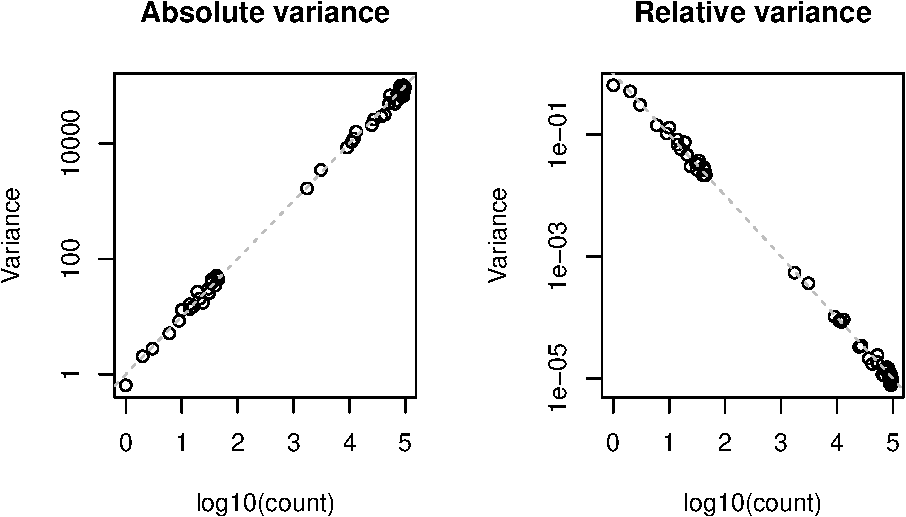
\includegraphics{_main_files/figure-latex/poisson-1.pdf}
\caption{\label{fig:poisson}Variance in constrained data is not what we
expect. Numbers between 1 and 1000 were generated (the sample) and
converted to 50 random instances using a multivariate Poisson process by
sampling from the Dirichlet distribution (the instances). The absolute
variance of 50 random instances was determined and plotted as the
absolute variance of the instances vs.~the sample count value. The data
was transformed by converting each count to the ratio of the instance
count to the sample count (relative value) and the variance of these
relative values were plotted. The relative variance is greatest at the
low count margin and smallest at the high count margin as is observed
for actual sequencing data (Fernandes et al.
\protect\hyperlink{ref-fernandes:2013}{2013}; {\textbf{???}}).}
\end{figure}

We observed that \(\epsilon\) can be exponentially larger than \(\nu\)
at the low count margin when measured on a relative scale (Fernandes et
al. \protect\hyperlink{ref-fernandes:2013}{2013}; Gloor, Macklaim, et
al. \protect\hyperlink{ref-gloorAJS:2016}{2016}), and that properly
accounting for this realization alone can result in an excellent fit to
even problematic data. Thus, a reliable analysis can be obtained by
incorporating an `in silico' technical replication which explicitly
models the variation in \(\epsilon\) as a probability density function
on a per feature, per sample basis; in other words that
\(\tau_{j} = \nu_j + f(\epsilon_{j})\). This approach is implemented in
the ALDEx2 Bioconductor package and substantially reduces the false
positive identification rate in microbiome and transcriptome data while
maintaining an acceptable true positive identification rate (Thorsen et
al. \protect\hyperlink{ref-Thorsen:2016aa}{2016}).

The differences between groups, dispersion within groups and relative
abundance were calculated using the ALDEx2 R package that uses Bayesian
modelling that generates a probability function for \(\epsilon_j\) that
can be used to place bounds on the uncertainty of the the observed data
(Fernandes et al. \protect\hyperlink{ref-fernandes:2013}{2013}; Gloor,
Macklaim, et al. \protect\hyperlink{ref-gloorAJS:2016}{2016}). If there
are two groups, A and B, this requires that the data comparison is
properly centred on the difference between these groups. ALDEx2 has been
shown to give meaningful and reproducible results, even on sparse,
asymmetric datasets using many different experimental designs (Fernandes
et al. \protect\hyperlink{ref-fernandes:2013}{2013},
\protect\hyperlink{ref-fernandes:2014}{2014}; Macklaim et al.
\protect\hyperlink{ref-macklaim:2013}{2013}; McMurrough et al.
\protect\hyperlink{ref-mcmurrough:2014}{2014}), although as shown here
the asymmetry can still affect the outcome.

The starting point for analysis is an \emph{n} samples \(\times D\)
features array. The sample vector contains the number of reads mapped to
any of the \(j\) features in the \(i^{th}\) sample,
\(\textbf{s}_i=[j_1,j_2 \ldots j_D]\), where
\(i=1 \ldots n , j=1 \ldots D\). The total number of counts is
irrelevant and determined by the machine (Gloor and Reid
\protect\hyperlink{ref-Gloor:2016cjm}{2016}; Gloor, Wu, et al.
\protect\hyperlink{ref-gloor2016s}{2016}). These data are compositional
and are an example of an equivalence class with
\(\alpha_{i} = \sum \textbf{s}_{i}\). In theory, the vector
\(\textit{\textbf{s}}_i\) can be adjusted to a unit vector of
proportions, \({\textit{\textbf{p}}_i=[p_1,p_2 \ldots p_D] }\), i.e.
\(\alpha=1\), without loss of information by the maximum likelihood (ML)
estimate \(\textit{\textbf{p}}_i=\textit{\textbf{s}}_i / \alpha_{i}\).
In this representation, the value of the \(j^{th}\) feature is a ML
estimate of the probability of observing the counts conditioned on the
fractional \(f\) that the feature represents in the underlying data and
on the total read depth for the sample; i.e.,
\(\mathbb{P}_{i,j}(f_{i,j}|\alpha_i)\). However, the maximum likelihood
estimate will be exponentially inaccurate when the dataset contains many
values near or at the low count margin (Newey and McFadden
\protect\hyperlink{ref-Newey:1994}{1994}) as is common in sparse HTS
data. Instead we use a standard Bayesian approach (Jaynes and Bretthorst
\protect\hyperlink{ref-Jaynes:2003}{2003}) to infer a posterior
distribution of the unit vector directly from \(\textit{\textbf{s}}_i\),
by drawing \(k\) random Monte-Carlo instances from the Dirichlet
distribution with a uniform, uninformative prior of 0.5, i.e.:

\parbox[b]{7in}{
\begin{equation}
\textrm{P}_{i (1 \ldots k)}=
\left( \begin{array}{c}
    \textit{\textbf{p}}_1 \\
   \textit{\textbf{p}}_2 \\
    \vdots \\
    \textit{\textbf{p}}_k \\
\end{array} \right)=
\left( \begin{array}{ccccc}
    p_{i,11} & p_{i,21} & p_{i,31} & \dots  & p_{i,D1} \\
    p_{i,12} & p_{i,22} & p_{i,32} & \dots  & p_{i,D2} \\
    \vdots & \vdots & \vdots & \ddots & \vdots \\
    p_{i,1k} & p_{i,2k} & p_{i,3k} & \dots  & p_{i,Dk}\\
\end{array} \right)
\sim Dirichlet_{(1 \ldots k)}(\textit{\textbf{s}}_i + 0.5)
\label{eq:matrix}
\end{equation}
}

This approach has consistent sampling properties and removes the problem
of taking a logarithm of 0 when calculating the CLR because the count 0
values are replaced by positive non-zero values that are consistent with
the observed count data (Fernandes et al.
\protect\hyperlink{ref-fernandes:2013}{2013}; Gloor, Macklaim, et al.
\protect\hyperlink{ref-gloorAJS:2016}{2016}). Each of the Monte-Carlo
instances, by definition, conserves proportionality and accounts for the
fact that there is more information when \(\alpha_i\) is large than when
it is small. This partially restores scale invariance to the data by
providing a distribution of values where the uncertainty of features
scales inversely with the read depth (Fernandes et al.
\protect\hyperlink{ref-fernandes:2013}{2013}; Gloor, Macklaim, et al.
\protect\hyperlink{ref-gloorAJS:2016}{2016}).

The apparent solution to the sequencing depth problem is to normalize
the read count values across samples in some way. One method of
normalization to is by subsampling, often termed rarefaction, as this is
observed to reduce the influence of sequencing depth on variation in
\(\alpha\) and \(\beta\) diversity metrics (Horner-Devine et al.
\protect\hyperlink{ref-Horner-Devine:2004aa}{2004}; Weiss et al.
\protect\hyperlink{ref-Weiss:2017aa}{2017}). Another is to convert the
data to proportions or percentages; these latter values are widely
spoken of in the literature as `relative abundances'. Subsampling is
frequently used to estimate the associated sampling error. Some groups
have begun advocating the use of normalization methods prevalent in the
RNA-seq field (McMurdie and Holmes
\protect\hyperlink{ref-McMurdie:2014a}{2014}) but still treat the data
as point estimates of the true abundance. There are many other
normalizations that are used in the ecological and high throughput
sequencing literature and the purpose and effect of these on simulated
data are explored in the section on Data Transformations.

\hypertarget{CoDa}{%
\chapter{DNA sequencing data are compositions}\label{CoDa}}

\hypertarget{high-throughput-sequencing-generates-compositional-data}{%
\section{High throughput sequencing generates compositional
data}\label{high-throughput-sequencing-generates-compositional-data}}

In the Chapter \ref{sequencing} we saw that the capacity of the
sequencing instrument imposed an upper bound on the total number of
fragments that could be obtained from a given sequencing run. We also
saw that the process of sequencing is essentially a random sampling of
an environment where the environment contains more fragments than can
possibly be sequenced in Chapter \ref{random}. Finally, the data
obtained are read counts per genetic interval (gene or OTU) per sample.

The read counts per sample range from 0 to, as a maximum, the total
number of reads in the sample. Thus the data are positive integer data
with an arbitrary maximum. While the data have an arbitrary maximum, the
majority of current tools assume the data are counts and ignore the
arbitrary maximum constraint. This assumption is the basis of methods
grounded in distributions such as the zero inflated Gaussian (ZIG)
(Paulson et al. \protect\hyperlink{ref-Paulson:2013aa}{2013}), negative
binomial (Robinson, McCarthy, and Smyth
\protect\hyperlink{ref-Robinson:2010}{2010}) and Poisson based models
(Auer and Doerge \protect\hyperlink{ref-auer:2011}{2011}). Recent
benchmarking has demonstrated that such methods are unpredictable when
dealing with highly sparse data (Thorsen et al.
\protect\hyperlink{ref-Thorsen:2016aa}{2016}), do not control the false
discovery rate (Gloor, Macklaim, et al.
\protect\hyperlink{ref-gloorAJS:2016}{2016}; Hawinkel et al.
\protect\hyperlink{ref-hawinkel2017}{2017}), and behave poorly when
un-constrained datasets are examined (Fernandes et al.
\protect\hyperlink{ref-fernandes:2013}{2013}; {\textbf{???}}; Gloor,
Macklaim, et al. \protect\hyperlink{ref-gloorAJS:2016}{2016}).

Data of this type are called count compositions, and a number of groups
have started to work on developing appropriate methods to deal with high
throughput datasets as count compostions (Friedman and Alm
\protect\hyperlink{ref-Friedman:2012}{2012}; Fernandes et al.
\protect\hyperlink{ref-fernandes:2013}{2013},
\protect\hyperlink{ref-fernandes:2014}{2014}; Lovell et al.
\protect\hyperlink{ref-Lovell:2015}{2015}; Mandal et al.
\protect\hyperlink{ref-ancom:2015}{2015}; Kurtz et al.
\protect\hyperlink{ref-Kurtz:2015}{2015}; Gloor and Reid
\protect\hyperlink{ref-Gloor:2016cjm}{2016}; Erb and Notredame
\protect\hyperlink{ref-erb:2016}{2016}; Gloor, Wu, et al.
\protect\hyperlink{ref-gloor2016s}{2016}; Tsilimigras and Fodor
\protect\hyperlink{ref-Tsilimigras:2016aa}{2016}; Washburne et al.
\protect\hyperlink{ref-Washburne:2017aa}{2017}; T. Quinn et al.
\protect\hyperlink{ref-Quinn:2017}{2017}; Silverman et al.
\protect\hyperlink{ref-Silverman:2017aa}{2017}; T. P. Quinn et al.
\protect\hyperlink{ref-Quinn206425}{2017}; Kaul et al.
\protect\hyperlink{ref-Kaul:2017aa}{2017}; Erb et al.
\protect\hyperlink{ref-Erb134536}{2017}; Egozcue, Pawlowsky-Glahn, and
Gloor \protect\hyperlink{ref-egozcue:AJS}{2018}).

So what is compositional data (CoDa), and what are its properties with
respect to high throughput sequencing that make this an important issue?

\hypertarget{compositional-data}{%
\section{Compositional data}\label{compositional-data}}

Data from high throughput sequencing have the following properties; the
data are counts, the data are non-negative, and the data has an upper
bound imposed by the instrument. This fits with the definition of
compositional data: compositional data contain \(D\) features (OTUs,
genes, etc), where the count of each feature is non-negative, and the
sum of the parts is known or arbitrary (Aitchison
\protect\hyperlink{ref-Aitchison:1986}{1986}, pg25). Note that the data
do not have to sum to a predetermined amount, it is sufficient that the
sum of the parts be known and be bounded.

A vector containing \(D\) features where the sum is 1 can be formally
stated as:
\(\vec{X} = \{(x_1,x_2,x_3, \ldots x_D); x_i\ge 0; \sum_{x=1}^{D} = 1\}\).
The sum of the parts is usually set to 1 or 100, but can take any value;
i.e., any composition can be scaled to any arbitrary sum such as a ppm.
Compositional data are equivalence classes since one vector can be
scaled into another through multiplication by an arbitrary constant
(Barceló-Vidal, Martín-Fernández, and Pawlowsky-Glahn
\protect\hyperlink{ref-barcelo:2001}{2001}). In the lexicon of high
throughput sequencing the vector is the sample and the features are the
OTUs or genes or genomic intervals. The total sum is the total number of
fragments observed for the sample; i.e., the sequencing depth.

\hypertarget{coda-pathologies}{%
\section{CoDa pathologies}\label{coda-pathologies}}

Compositional data have a number of built-in pathologies: a negative
correlation bias, sub-compositional incoherence, and spurious
correlations. A proper analysis of compositional data must as a minimum
account for these pathologies.

Formally, compositional datasets have the property that they are
described by \(D-1\) features (Aitchison
\protect\hyperlink{ref-Aitchison:1986}{1986}). In other words, if we
know that all features sum to a constant, then the value of any
individual feature can be known by subtracting the sum of all other
parts from that constant; i.e., \(x_D = 1-\sum_{x=1}^{D-1}\).

Graphically, this means that compositional data inhabit a space called a
Simplex that contains 1 fewer dimensions than the number of features.
The distances between parts on the Simplex are not linear. This is
important because all parametric statistical tests assume that
differences between parts are linear (or additive). Thus, while standard
tests will produce output, the output will be misleading because
distances on the simplex are non-linear and bounded (Martín-Fernández et
al. \protect\hyperlink{ref-martin1998measures}{1998}). Chapter
\ref{transforms} on Data Transformations contains an intuitive
demonstration of how data are moved to the Simplex when a the data are
compositional.

It is not always apparent when the data are compositional. This is
especially true for large multivariate datasets such as those generated
in high throughput sequencing. Aitchison
(\protect\hyperlink{ref-Aitchison:1986}{1986}) indicated that a
compositionally appropriate analysis should fulfil a number of
properties, and when these properties are not met with traditional
analyses, the data are likely compositional.

\begin{itemize}
\item
  A compositionally appropriate analysis should be scale invariant, that
  is, the results should not depend on the total count or scale of the
  sample. This first principle of CoDa data analysis indicates that all
  count normalization, or sequencing depth adjustments are either
  unnecessary or counterproductive. There is substantial resistance to
  the idea the high throughput sequencing data are compositional, and
  indeed many analysts believe that the data can be made
  non-compositional with the `correct' transform that restores the
  scale. The is belief is exposed to be false in Chapter
  \ref{transforms}.
\item
  A compositionally appropriate analysis should also not depend on the
  order of the features in the dataset. This almost goes without saying,
  but is included because of the way that one particular transformation,
  the alr, was formulated.
\item
  A compositionally appropriate analysis should exhibit subcompositional
  coherence, or the results of analysis of a sub-composition should be
  the same as for the entire composition. In practice, this is difficult
  to achieve, and we settle for least sub-compositional dominance where
  the distances between features in the full composition are equal to or
  greater than the distances in the sub-composition. In later chapters
  where we examine real datasets, I show how to determine if
  sub-compositional dominance is fulfilled by the analysis.
\end{itemize}

\hypertarget{negative-correlation-bias-in-compositions}{%
\subsection{Negative correlation bias in
compositions}\label{negative-correlation-bias-in-compositions}}

\begin{picture}(100,50)(0,0)
    \put(50,25){V}
    \put(142,25){M}
    \put(100,5){\vector(0,1){12} }
    \put(50,20){\line(1,0){100}}
\end{picture}

The values of the parts of compositional datasets are constrained
because of the constant sum, and this constraint has been known for a
very long time {[}({\textbf{???}});1896{]}. The features in a
composition have a negative correlation bias since an increase in the
value of one part must be offset by a decrease in value of one or more
other parts. In the illustration above, we see that `V' and `M' are
perfectly balanced on the fulcrum because they have the same mass. If M
becomes heavier, then V will rise even though the mass of V has not
changed. The same principle operates in compositional data. If V is the
amount of money spend on vegetables, and M is the amount of money spent
on meat, and the total food budget is a constant, then the only way that
more meat could be consumed would be to spend less on vegetables.
Therefore, the amount of money spent on V and M will be perfectly
negatively correlated if the total food budget is constrained. This
example generalizes to any number of items in the shopping basket as
long as the total budget is constrained. When there are more items, then
an increase in one item (say shoes) must be offset by a decrease in
another item, but it could be a decrease in meat, vegetables or both.

\hypertarget{spurious-correlations}{%
\subsection{Spurious correlations:}\label{spurious-correlations}}

In addition to a negative correlation bias, compositional data has the
problem of spurious correlation (Pearson
\protect\hyperlink{ref-Pearson:1896}{1897}); in fact spurious
correlation was the first troubling issue identified with compositional
data. This phenomenon is best illustrated with the following example
from Lovell et. al (\protect\hyperlink{ref-Lovell:2015}{2015}), where
they show how simply dividing two sets of random numbers (say abundances
of OTU1 and OTU2), by a third set of random numbers (say abundances of
OTU3) results in a strong correlation. Note that this phenomenon depends
only on there being a common denominator.

\begin{Shaded}
\begin{Highlighting}[]
\NormalTok{n.obs <-}\StringTok{ }\DecValTok{100}
\NormalTok{OTU.df <-}\StringTok{ }\KeywordTok{data.frame}\NormalTok{(}
    \DataTypeTok{OTU1=}\KeywordTok{rnorm}\NormalTok{(n.obs, }\DataTypeTok{mean=}\DecValTok{10}\NormalTok{, }\DataTypeTok{sd=}\DecValTok{1}\NormalTok{),}
    \DataTypeTok{OTU2=}\KeywordTok{rnorm}\NormalTok{(n.obs, }\DataTypeTok{mean=}\DecValTok{10}\NormalTok{, }\DataTypeTok{sd=}\DecValTok{1}\NormalTok{),}
    \DataTypeTok{OTU3=}\KeywordTok{rnorm}\NormalTok{(n.obs, }\DataTypeTok{mean=}\DecValTok{30}\NormalTok{, }\DataTypeTok{sd=}\DecValTok{4}\NormalTok{))}
\NormalTok{OTU.df <-}\StringTok{ }\KeywordTok{transform}\NormalTok{(OTU.df,}
    \DataTypeTok{OTU1.over.OTU3=}\NormalTok{ OTU1}\OperatorTok{/}\NormalTok{OTU3,}
    \DataTypeTok{OTU2.over.OTU3=}\NormalTok{ OTU2}\OperatorTok{/}\NormalTok{OTU3)}
\KeywordTok{plot}\NormalTok{(OTU.df}\OperatorTok{$}\NormalTok{OTU1.over.OTU3,}
\NormalTok{    OTU.df}\OperatorTok{$}\NormalTok{OTU2.over.OTU3, }\DataTypeTok{pch=}\DecValTok{19}\NormalTok{,}
    \DataTypeTok{cex=}\FloatTok{0.3}\NormalTok{,}\DataTypeTok{xlab=}\StringTok{"OTU1/OTU3"}\NormalTok{,}
    \DataTypeTok{ylab=}\StringTok{"OTU2/OTU3"}\NormalTok{)}
\end{Highlighting}
\end{Shaded}

\begin{figure}
\centering
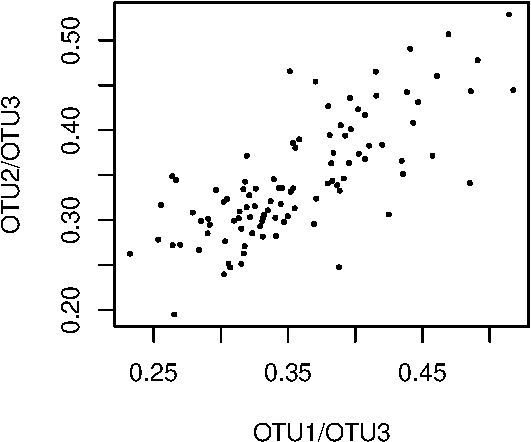
\includegraphics{_main_files/figure-latex/correlation-1.pdf}
\caption{\label{fig:correlation}Spurious correlation in compositional data.
Two random vectors drawn from a Normal distribution, were divided by a
third vector also drawn at random from a Normal distribution. The two
vectors have nothing in common, they should exhibit no correlation, and
yet they exhibit a correlation coefficent of \(>0.65\) when divided by
the third vector. See the introductory section of the Supplementary
Information of Lovell (\protect\hyperlink{ref-Lovell:2015}{2015}) for a
more complete description of this phenomenon.}
\end{figure}

\hypertarget{sub-compositions}{%
\subsection{Sub-compositions}\label{sub-compositions}}

Compositional data have the third property of sub-compositional
incoherence of correlation metrics as illustrated in Chapter
\ref{transforms}. That is,
\emph{correlations calculated on compositional datasets are unique to the particular dataset chosen}
(Aitchison \protect\hyperlink{ref-Aitchison:1986}{1986}). This is
problematic because high throughput sequencing experimental designs are
\emph{always} sub-compositions. Inspection of papers in the literature
provide many examples. For example, in the 16S rRNA gene sequencing
literature it is common practice to discard rare OTU species prior to
analysis and to re-normalize by dividing the counts for the remaining
OTUs by the new sample sum. It is also common to use only one or a few
taxonomic groupings to determine differences between experimental
conditions. In the case of RNA-seq only the fraction of RNA of interest
is sequenced, usually mRNA but other sub-fractions such as miRNA may be
sequenced. All of these practices expose the investigator to the problem
of non-coherence between sub-compositions. We must use
compositionally-appropriate measures of correlation---more formally, we
are attempting to find features that are compositionally associated.
Compositional association as a more restricted measure of correlation
and is explained more completely in the chapter on data transformations.

To summarize, compositional data has the following pathologies:

\begin{itemize}
\item
  The negative correlation bias means that any negative correlation
  observed in compositional data must be treated as suspect because it
  could arise simply because a different feature (or features) changed
  their abundance. There is currently no theoretically valid approach to
  identify true negative correlations in compositional data (Egozcue,
  Pawlowsky-Glahn, and Gloor \protect\hyperlink{ref-egozcue:AJS}{2018}).
\item
  The spurious correlation problem means that we can observe apparent
  postive correlations simply by chance. I describe recent work that
  shows that spurious correlation is tractable.
\item
  The sub-compositional incoherence of correlation is perhaps the most
  insidious property, but also the easiest to recognize. Here the
  correlation depends on the \emph{exact} set of features present in the
  dataset. If the observed correlations change when the data are subset,
  then sub-compositional incoherence is in play.
\end{itemize}

Thus, one major reason to use compositional data methods is that you are
more likely to report robust results, and the later practical chapters
demonstrate the robustness of a compositional data analysis.

Practically speaking the negative correlation bias, the occurrence of
spurious correlation, and the problem of sub-compositional incoherence
means that
\emph{every microbial correlation network that has ever been published is suspect},
as is \emph{every gene co-occurrence or co-expression network} unless
compositionally appropriate compositional association metric was used
(Lovell et al. \protect\hyperlink{ref-Lovell:2015}{2015}; Erb and
Notredame \protect\hyperlink{ref-erb:2016}{2016}; T. P. Quinn et al.
\protect\hyperlink{ref-Quinn206425}{2017}). These approaches themselves
have limitations and as originally constituted cannot deal with sparse
data. However, recasting the data from count compositions to probability
distributions allows these methods to be adapted to sparse data with
some success (Bian et al., \protect\hyperlink{ref-bian:2017}{n.d.}; T.
P. Quinn et al. \protect\hyperlink{ref-Quinn206425}{2017}).

\hypertarget{so-can-i-analyze-compositional-data-how}{%
\section{So can I analyze compositional data?
How?}\label{so-can-i-analyze-compositional-data-how}}

Much of the high throughput sequencing analysis literature seems to
assume that data derived from high throughput sequencing are in some way
unique, and that purpose-built tools must be used. However, there is
nothing special about high-throughput sequencing data from the point of
view of the analysis. Fortunately, the analysis of compositional
datasets has a well-developed methodology (Pawlowsky-Glahn, Egozcue, and
Tolosana-Delgado \protect\hyperlink{ref-pawlowsky2015modeling}{2015};
Van den Boogaart and Tolosana-Delgado
\protect\hyperlink{ref-van2013}{2013}), much of which was worked out in
the geological sciences.

Atichison (\protect\hyperlink{ref-Aitchison:1986}{1986}), Pawlsky-Glahn
(\protect\hyperlink{ref-Pawlowsky-Glahn:2006}{2006}), and Egozcue
(\protect\hyperlink{ref-egozcue2005}{2005}), have done much work to
develop rigorous approaches to analyze compositional data
(Pawlowsky-Glahn and Buccianti
\protect\hyperlink{ref-pawlowsky2011compositional}{2011}). The essential
step is to reduce the data to ratios between the \(D\). This step does
not move the data from the Simplex but does transform the data on the
Simplex such that the distances between the ratios of the features are
linear. The investigator must keep in mind that the distances are
between ratios between features, not between counts of features (re-read
this several times to wrap your head around it). Several transformations
are in common use, but the one I believe is most applicable to HTS data
is the centred log-ratio transformation or clr. The clr, and other
common data transformations are explained in the next Chapter---I bet
you can't wait!

\hypertarget{basic-idea-of-coda-analysis}{%
\subsection{Basic idea of CoDa
analysis}\label{basic-idea-of-coda-analysis}}

We want to answer the question: Have the abundances of the taxa changed?
But we cannot, because as we have seen the actual abundances are not
available. Instead we have relative abundances, that is the ratios
between the features, and the following is a simple example.

We sequence, and have a total count of about 100 (it is a second
generation GregSeq machine!)

So we get: \begin{math}A_s = [71,7,4,18], B_s = [1,25,12,62]
\end{math}

Note that these values appear to be very different between the groups.
However, if we take one feature as a reference, say feature 4, and
determine a ratio, i.d.:

\begin{math}
A_r = [ 74/18, 7/18, 4/18 ] = [ 4.1, 0.39, 0.22 ]
\end{math}

\begin{math}
B_r = [ 1/62, 25/62, 12/62 ] = [ 0.02 , 0.40, 0.20 ]
\end{math}

Here we can see that if we assume one feature is constant (feature 4),
then the last two are seen to be very similar in abundance relative to
feature 4. Now we can infer that the majority of change is in the first
feature assuming feature 4 is invariant. We cannot compare the last
feature because it is assumed to be constant, that is, the assumed
change in the last feature is 0. This approach is the one used by ANCOM,
a recently developed tool to assess change in microbiome datasets
(Mandal et al. \protect\hyperlink{ref-ancom:2015}{2015}).

Since we cannot know which feature, if any, is constant, we can assume
that a large number of the taxa exhibit only random change. Then rather
than using one feature as a reference we can use the geometric mean
abundance of all features. Note: this approach works poorly if there are
only a small number of taxa (less than about 50) or if the taxa are very
asymmetrically distributed between groups. This approach is the one used
by ALDEx2 (Fernandes et al.
\protect\hyperlink{ref-fernandes:2013}{2013},
\protect\hyperlink{ref-fernandes:2014}{2014}), and is the method that we
will use.

One complication is that a genometric mean cannot be determined if any
of the values have a count of 0. For pairwise comparisons

\hypertarget{transforms}{%
\chapter{Data transforms in high throughput
sequencing}\label{transforms}}

This chapter introduces data transformations and distance (or
dissimilarity) metrics that are prevalent in the ecological literature,
and that have been extensively used in analyzing high throughput
sequencing datasets. It is not intended to be a comprehensive analysis
of data transformations. In some cases, only one transformation is
demonstrated when several transformations are obviously related.

This chapter is rather information dense, but the lessons in it are very
important to understand the limitations of data analysis whenever the
data are compositional. I have tried to make it easy and intuitive, but
in the end you must work through the examples as best you can. All the
source code needed to explore the data are included either directly
here, or in an external file when the amount of code would break the
flow of the narrative.

\hypertarget{why-transform-data}{%
\section{Why transform data?}\label{why-transform-data}}

Data are transformed for a variety of reasons. The first reason, is to
make the data amenable to statistical assumptions for parametric tests
that require the data be normally distributed with similar standard
deviations in all groups. Can we transform the data to approximate a
Gaussian distribution? This mode of thinking leads to the use of
square-root, arcsine or Hellinger transformations since they appear to
transform the data into a distribution that can be interpreted. However,
as we shall see below, none of these univariate transformations is
suitable, and many of these historically common transformations have
recently fallen out of favour, e.g., (Warton and Hui
\protect\hyperlink{ref-Warton:2011aa}{2011}).

The logaritmic transformation is now commonly used after one of the
`count normalization' methods described below. As we shall see below,
neither count normalized, nor log count normalized data is generally the
best option. The second reason for normalization is to remove or adjust
the compositional nature of the data (Weiss et al.
\protect\hyperlink{ref-Weiss:2017aa}{2017}), again, as we shall see this
is not possible. The assumption is that any conclusion made on the
transformed data represents in some way changes in the underlying
abundance of the input DNA molecules as outlined in Chapter
\ref{sequencing}. As we shall see, this is not possible, but using a
CoDa-based approach we can determine if changes in the
\emph{relative values} of DNA molecules are altered; the question is
``relative to what?''.

Fundamentally, the goal of any experiment is to determine something
about the environment that was sampled. After all, we are attempting to
use HTS to determine something of interest about the underlying
environment. Thus, we need to have some equivalence between the samples
before sequencing and the samples after sequencing. The simplest case
would be that there would be a linear relationship between the data that
we could obtain from the environment, and the data that was actually
collected by HTS.

\hypertarget{sequencing-changes-the-shape-of-all-but-the-most-ideal-data}{%
\section{Sequencing changes the shape of all but the most ideal
data:}\label{sequencing-changes-the-shape-of-all-but-the-most-ideal-data}}

We have seen that high throughput sequencing as currently practiced is
constrained by the capacity of the instrument. Let us revisit the toy
example in Figure \ref{shape}, where we had an unconstrained random
sample of counts and see how well common data transformations work to
recapitulate the overall shape of the data.

the In this section I show that the practical consequence of the
instrument constraint can be severe in all but the most idealized
datasets. An idealized dataset is one where the total number of
molecules is the same per sampling effort in all the samples taken from
the the environment. An example of such an idealized would be if the
samples were taken from a cell culture experiment with a treatment and
control group where the treatment was expected to alter only a small
number of features. This would be an example of a constrained dataset:
the total number of DNA molecules in the samples in the two groups would
be expected to be substantially the same except for random variation.
This assumption is implicit in all differential abundance tools in use.

An example of a less than ideal experiment would be comparing the total
gene content in DNA isolated from two different ecosystems.

It is more desirable to think about HTS data in a multivariate way as a
`composition' because the total count of molecules in the underlying
sample (the environment) is always a confounding variable (Lovén et al.
\protect\hyperlink{ref-Loven:2012aa}{2012}). This way of thinking led to
multivariate data normalizations.

\hypertarget{commonly-used-transformations-are-misleading}{%
\section{Commonly used transformations are
misleading}\label{commonly-used-transformations-are-misleading}}

The \texttt{vegan} R package manual (Oksanen et al.
\protect\hyperlink{ref-vegan:2017}{2017}) has a very good description of
many data transformations and I recommend it to the interested reader:
note that the transforms in the \texttt{vegan} package are not
compositionally appropriate, and I do not recommend them in general for
the reasons outlined below.

Current practice is to examine the datasets using `relative abundance'
values, that is, the proportional abundance of the features either
before or after normalization for read depth. This approach is
equivalent to examining the input unconstrained data of the type seen in
Figure \ref{fig:shape} in the relative abundance sample space in the
bottom right panel of the figure after normalizing the total number of
reads to be approximately constant. This approach will obviously lead to
incorrect assumptions in at least some cases. For example, depending
upon the steps chosen to compare, the blue feature, that has constant
counts in the input, will be seen to either increase or decrease in
abundance. Conversely, the black feature, that is always decreasing in
abundance will be seen to be constant if comparing samples 1-8.

\begin{figure}
\centering
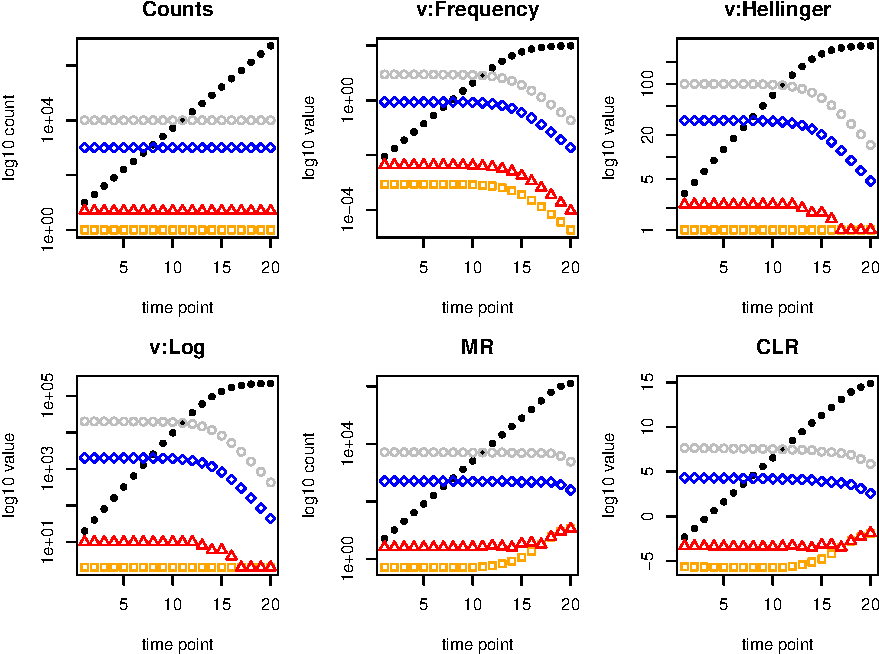
\includegraphics{_main_files/figure-latex/transformations-1.pdf}
\caption{\label{fig:transformations}The effect of ecological transformations
on unconstrained high throughput sequencing datasets. Data generated as
in Figure \ref{fig:shape} were normalized to a (near) constant total
number of reads, converted to proportions, then transformed with five
different approaches implemented in the vegan ecological analysis
package. The `Counts' panel shows the original data, the other panels
begin with a `v:' and indicate the vegan package transformation. The
transformation in the MR panel is described below.}
\end{figure}

The ecological literature offers many different transformations for such
data, often as a way of making the data appear `more normal'. Figure
\ref{fig:transformations} shows the results of a few such
transformations that are in the \texttt{vegan\ R} package.

\begin{itemize}
\item
  The frequency transform divides the each feature value by the largest
  feature count, and then divides the resulting values by the number of
  features in the sample that had non-zero counts. This is the often
  referred to as `relative abundance' and is a simple proportion.
\item
  The Hellinger transformation that takes the square root of the
  relative abundance (proportion) value.
\item
  The log transform divides each feature count in a sample by the
  minimum non-zero count value, then takes the logarithm of the
  resulting value and adds 1. Counts of 0 are assigned a value of 0 to
  avoid taking the logarithm of 0.
\end{itemize}

The MR and CLR transforms are not instantiated in \texttt{vegan}, and
are described below.

It is obvious that the Frequency, Hellinger, and Log transformations
result in data that badly mis-represents the shape of the actual count
data. All other transformations instantiated in the \texttt{vegan}
package deliver data that is transformed even more extremely. The log
transformation would be suitable \emph{if} the total counts observed
after sequencing was directly proportional to the total counts in the
enviroment, however, we have seen that this condition cannot be met for
high throughput sequencing. Thus, none of these transformations, though
widely used, are suitable when analyzing high throughput sequencing
data.

The MR and CLR transforms appear to most closely recapture the shape of
the original data and appear very similar. We will discuss these below.

Comparison of `differential abundance' is problematic for compositional
data (Fernandes et al. \protect\hyperlink{ref-fernandes:2013}{2013},
\protect\hyperlink{ref-fernandes:2014}{2014}). Since the apparent
abundance of every value depends on the apparent abundance of every
other value, we can get into real difficulties if we are not careful. If
we refer back to Figure \ref{fig:transformations}:Counts, and we compare
the relative abundances of features between sample 1 and sample 20, we
observe that only the black feature has changed in absolute abundance
and that the count of all other features is unchanged. Note that we
would be very wron in our inferences if we use the Frequency, Hellinger
or Log transforms, since we would infer that the black feature
increased, but that all other features had decreased in abundance. The
MR and CLR transformations do a better job of controlling for the
interdependence between features. Both transforms have the black feature
increasing, but the other features increase or decrease only marginally,
and apparently at random.

\hypertarget{other-data-transformations}{%
\section{Other data transformations}\label{other-data-transformations}}

I will introduce each of the transformations in turn, and then we will
examine the effect of each transformation on the data. Let us see which,
if any of the transforms fulfills the basic requirements set out above.

\hypertarget{notation}{%
\subsection{Notation}\label{notation}}

We use the following notation throughout.

\begin{itemize}
\tightlist
\item
  Column vectors contain samples \(\vec{\textbf{s}}\) and row vectors
  contain features \(\vec{\textbf{f}}\)
\item
  There are \(D\) features and \(n\) samples, thus the data are
  contained in matrix of dimension \(M = D \times n\)
\item
  The \(j^{th}\) sample is denoted as \(\vec{\textbf{s}}_{j}\)
\item
  The \(i^{th}\) feature of all samples is denoted as
  \(\vec{\textbf{f}}_{i-}\)
\item
  The value for the \(i^{th}\) feature of the \(j^{th}\) sample is
  referred to as \(s_{ij}\) We will consider the following
  transformations
\end{itemize}

\hypertarget{the-proportional-transformation}{%
\subsection{The proportional
transformation}\label{the-proportional-transformation}}

This simple normalization is to determine the relative abundance (rAB),
or proportion, of the \ith{i} feature in a sample as in Eq.
\ref{eq:rab}. This normalization is also referred to as the total sum
scaling (TSS) normalization. The effect is shown in panel Frequency in
Figure \ref{fig:transformations}.

\begin{equation}
    rAB_{i} = \frac{s_{i}}{\sum{\vec{\textbf{s}}}}
    \label{eq:rab}
\end{equation}

The rAB measure requires only the read count observed for the feature
\(s_{ij}\) and the total read count of the sample
\(\sum{\vec{\textbf{s}}}\). Since this measure is generally skewed, it
is often log-transformed prior to analysis.

\hypertarget{the-rpkm-and-tpm-transformations}{%
\subsection{The RPKM and TPM
transformations}\label{the-rpkm-and-tpm-transformations}}

A further normalization was proposed early in the RNA-seq field where
the reads per kilobase per million mapped (RPKM)(Mortazavi et al.
\protect\hyperlink{ref-Mortazavi:2008}{2008}) method was used initially
to place the read counts for each feature within and between samples on
a common scale.

For this we also needed to know a scaling factor \(K\), and the length
of the feature \(L_i\); from this, the RPKM value for the \ith{i}
feature for each sample was calculated as in Eq. \ref{eq:rpkm}.

\begin{equation}
    RPKM_{i} = \frac{K \cdot s_{i} }{\sum{\vect{s}} \cdot L_{i}}
    \label{eq:rpkm}
\end{equation}

When the equation is placed in this form it is obvious that RPKM is
simply a scaled rAB where each rAB value is divided by its length and
multiplied by a constant. In compositional terms, RPKM is an unclosed
perturbation of the original data; the data appear to be real numbers,
but are actually proportions multiplied by a constant.

Further research suggested that RPKM was not appropriate for comparison
of features between samples. The goal of RPKM was to `count' reads per
feature per cell. In the original paper the authors supplied an
equivalence and an RPKM value of 1 RPKM equalled one transcript in each
cell in the C2C12 cell line, but in liver cells, a value of 3 RPKM
equalled one transcript per cell. Thus, from the start, this
normalization was unable to normalize between-condition read counts.

The transcripts per million (TPM) normalization was advocated next (Li
et al. \protect\hyperlink{ref-Li:2010aa}{2010}). Patcher (Pachter
\protect\hyperlink{ref-Pachter:2011}{2011}) showed the equivalence
between RPKM and TPM, and in compositional terms TPM is simply a
compositionally closed form of RPKM multiple by a constant as in Eq.
\ref{eq:tpm}.

\begin{equation}
    TPM_{i} = \frac{RPKM_i}{\sum{RPKM}} \cdot K
    \label{eq:tpm}
\end{equation}

The rAB, RPKM and TPM normalizations are thus all very similar,
differing only in the scaling of individual features, and do not allow
normalization between conditions unless the samples in the environment
contain \emph{exactly} the same input number of RNA molecules. These
normalizations deliver proportional data, scaled or perturbed to make
the data appear as if they are numerical, and not proportional. Thus,
these transformations deliver data with the same properties as shown in
Figure \ref{fig:transformations}, except that the scale of the y axis is
altered.

A related transformation is `rarefaction' or subsampling without
replacement to a defined per-sample read count. This transformation was
widely used in the 16S rRNA gene sequencing field. Rarefaction to a
common read count gives a composition, that is scaled such that low
count features often are replaced by 0 values (McMurdie and Holmes
\protect\hyperlink{ref-McMurdie:2014a}{2014}). For this reason,
rarefaction has now been largely replaced with the median of ratios
method described below.

\hypertarget{the-median-of-ratios-count-normalization}{%
\subsection{The median of ratios count
normalization}\label{the-median-of-ratios-count-normalization}}

Further work found that none of these methods were appropriate, since
the read count per sample continued to confound the analyses (Lovén et
al. \protect\hyperlink{ref-Loven:2012aa}{2012}). In other words, the
TMM, RPKM, TPM methods \emph{are not scale invariant}.

Thus, the scaling normalization methods were proposed (White, Nagarajan,
and Pop \protect\hyperlink{ref-White:2009}{2009}; Robinson and Oshlack
\protect\hyperlink{ref-Robinson:2010a}{2010}), reviewed in (Dillies et
al. \protect\hyperlink{ref-Dillies:2013}{2013}). There are several
scaling normalizations, but all operate on the common assumption that by
normalizing all counts in a sample to a per-sample midpoint value the
normalization can impute, or at least approximate, the \emph{number} of
each feature in the underlying environment. The approaches differ
largely in how the midpoint is determined. The median of ratios method
(MR) is instantiated in DESeq2 (and others), the trimmed mean of M
values (TMM) method is used by edgeR (and others), and the Cumulative
Sum Scaling (CSS) method is used by metaGenomeSeq (White, Nagarajan, and
Pop \protect\hyperlink{ref-White:2009}{2009}) among others. The MR
method will be demonstrated and used, but the TMM and CSS methods give
substantially similar results, and uses the same basic logic since
sample values are linearly scaled by a per-sample feature-wise midpoint.

The MR method calculates the ratio of the features to the geometric
mean, \(\mathrm{g}\vect{f}_{i-}\), of each feature across all samples,
and then takes as the normalization factor the median ratio per sample
as the scaling factor. Each feature is then divided by the scaling
factor to place each sample on an `equivalent' count scale. The idea is
that the MR normalization `opens' the data from being compositional to
being scaled counts. It is impossible to open the data, and while the
scaled counts may have some useful properties, we see below that
removing compositional constraints are not among them.

The multi-step normalization MR normalization attempts to normalize for
sequencing depth thus `opening' the data, and proceeeds as in the
multistep Eq. \ref{eq:MR}. Here we start with two sample vectors
\(\vec{\textbf{s}}_1\) and \(\vec{\textbf{s}}_2\), and calculate a
vector of geometric means of the features \(\vec{\textbf{g}}\). Ratio
vectors, \(\vec{\textbf{r}}_j\) are calculated by dividing the sample
vectors by the geometric mean vector, and the median of the ratio
vectors is determined. Finally, the sample vectors are divided by the
median of the ratio vector for each sample.

\begin{equation}
    \begin{aligned}
        \vec{\textbf{g}} = &\ \mathrm{g}\vect{f}{i-}\\
        \vec{\textbf{r}}_j = &\ \vec{\textbf{s}}_j / \vec{\textbf{g}}\\
        \vec{\textbf{d}}_j = &\ \vec{\textbf{s}}_j / Md(\vec{\textbf{r}}_j)\\
    \end{aligned}
\label{eq:MR}
\end{equation}

A sample calculation is given in Table \ref{tab:des}, and we can see
that the median ratio for each sample \(\vec{\textbf{r}}_j\) samples may
be different in each sample, and that the particular feature that is the
median may itself be different, the median feature is in boldface in the
table. Thus, by construction the feature values in each sample can be
scaled by different amounts in each sample.

The MR normalization has the attractive property that it approaches the
shape of the underlying count data when the dataset is relatively well
behaved. We can see this in panel MR in Figure
\ref{fig:transformations}. Here, only the extreme samples at points
15-20 diverge strongly from the values observed in the underlying count
data. The MR normalization is now widely used in both the 16S rRNA gene
sequencing field {[}REF{]} and in the RNA-seq field {[}REF{]}. However,
we can see that the normalization fails at the margin without warning.
Thus, we can never be sure if we are comparing values correctly. An
additional issue is that the MR normalization is not compositionally
appropriate, and even though it (nearly) recapitulates the overall shape
of the data, it does not recapitulate the \emph{relationships} between
the data. Nevertheless, the MR transformation may be useful in ideal, or
nearly ideal cases if interpreted carefully.

\begin{table}[!h]
\caption{Example calculation of MR normalization}
\centering
\resizebox{\columnwidth}{!}{%
\begin{tabular}{c r r r r r r r}
\hline
Feature & $\vec{\textbf{s}}_1$ & $\vec{\textbf{s}}_2$ & $\vec{\textbf{g}}$ & $\vec{\textbf{r}}_1$ & $\vec{\textbf{r}}_2$ & $\vec{\textbf{d}}_1$ & $\vec{\textbf{d}}_2$ \\ \hline \hline
F1 & 1500 & 1000 & 1224.7 & 1.22 & {\bf 0.81} & 1219.5 & 1234.6\\
F2 & 25 & 15 & 19.4 & 1.29 & 0.77 & 20.3 & 18.5 \\
F3 & 1000 & 500 & 707.1 & 1.41 & 0.71 & 813.0 & 617.3 \\
F4 & 75 & 50 & 61.2 & {\bf 1.23} &  0.82 & 61.0 & 61.7 \\
F5 & 500 & 1500 & 866.0 & 0.58 & 1.73 & 406.5 & 1851.9\\ \hline
\end{tabular}
}
\label{tab:des}
\end{table}

\hypertarget{log-ratio-transformations}{%
\section{Log-ratio transformations}\label{log-ratio-transformations}}

Aitchison (\protect\hyperlink{ref-Aitchison:1986}{1986}) introduced the
concept of the log-ratio transformation.

There are three main log-ratio transformations; the additive log-ratio
(alr), centred log-ratio (clr) and the isometric log-ratio (ilr)
(Aitchison \protect\hyperlink{ref-Aitchison:1986}{1986};
Pawlowsky-Glahn, Egozcue, and Tolosana-Delgado
\protect\hyperlink{ref-pawlowsky2015modeling}{2015}).

Using the same notation as above for a sample vector
\(\vec{\textbf{s}}\) of \(D\) `counted' features (taxa, operational
taxonomic units or features, genes, etc.)
\(\vec{\textbf{s}}=[s_1, s_2, ... s_D]\):

The alr is the simply the elements of the sample vector divided by a
presumed invariant feature, which by convention here is the last one:

\begin{equation}
\begin{aligned}
 \vec{\textbf{x}}_{alr}= &\ [log(x_1/x_D), log(x_2/x_D), \\
 & \ldots log(x_D-1/x_D]
\end{aligned}
 \label{eq:alr}
\end{equation}

This is similar to the concept used in quantitative PCR, where the
relative abundance of the feature of interest is divided by the relative
abundance of a (presumed) constant `housekeeping' feature. Of course
there are two major drawbacks. First, that the experimentalist's
knowledge of which, if any, features are invariant is necessarily
incomplete. Second, is that the choice of the (presumed) invariant
feature has a large effect on the result if the presumed invariant
feature is not invariant, or if it is correlated with any other features
in the dataset. Interestingly, an early proposal was to use the
geometric mean of a number of internal controls (Vandesompele et al.
\protect\hyperlink{ref-Vandesompele:2002aa}{2002}), leading to the next
transformation.

\hypertarget{the-centered-log-ratio-transformation.}{%
\subsection{The centered log-ratio
transformation.}\label{the-centered-log-ratio-transformation.}}

The clr is performed by taking the logarithm of the the ratio between
the count value for each part and the geometric mean count: i.e., for D
features in sample vector \(\vect{s} = [s_1, s_2, s_3, \ldots s_D]\):

\begin{equation}
 \vect{s}_{clr}  = [log(\frac{s_1}{g\vect{s}}), log(\frac{s_2}{g\vect{s}}) \ldots log(\frac{s_D}{g\vect{s}})]
\end{equation}

where \(g\vect{s} = \sqrt[D]{x_1 \cdot x_2 \cdot ... \cdot x_D}\), the
geometric mean of \(\vec{\textbf{x}}\).

The clr transformation is formally equivalent to a matrix of all
possible pairwise ratios, but is a more tractable form.

The clr transform is scale invariant because the same clr values are
obtained from the raw counts and from the table of counts after
conversion to proportions. The clr transform is sub-compositionally
dominant (Pawlowsky-Glahn, Egozcue, and Tolosana-Delgado
\protect\hyperlink{ref-pawlowsky2015modeling}{2015}). Thus, the clr
transform fulfils the

The clr is often criticized since it has the property that the sum of
the clr vector must equal 0. This constraint causes a singular
covariance matrix; i.e., the sum of the covariance matrix is always a
constant (Pawlowsky-Glahn, Egozcue, and Tolosana-Delgado
\protect\hyperlink{ref-pawlowsky2015modeling}{2015}). However the clr
has the advantage of being readily interpretable, a value in the vector
is its abundance \emph{relative} to a mean value.

The ilr is the final transformation, and is a series of sequential
log-ratios between two groups of features. For example, the philr
transformation is the series of ratios between features partitioned
along the phylogenetic tree (Silverman et al.
\protect\hyperlink{ref-Silverman:2017aa}{2017}), although any other
sequential binary partitioning scheme is also possible (Pawlowsky-Glahn,
Egozcue, and Tolosana-Delgado
\protect\hyperlink{ref-pawlowsky2015modeling}{2015}). The ilr
transformation does not suffer the drawbacks of either the alr or clr,
but does not allow for insights into relationships between single
features in the dataset. Nevertheless, ilr transformations permit the
full-range of multivariate tools to be used, and are recommended
whenever possible.

The ilr and clr are directly comparable in a two important ways: First,
the distances between samples computed using an ilr and clr
transformation are equivalent. Second, the clr approaches the ilr in
other respects as the number of features becomes large. In this respect,
the large number of features---hundreds in the case of features,
thousands in the case of genes---in a typical experiment works in our
favour. Thus, while not perfect, the clr is the most widely used
transformation. However, care must be taken when interpreting its
outputs since single features must always be interpreted as a ratio
between the feature and the denominator used for the clr transformation.
The problems of using clr are apparent when some subcomposition or group
of taxa is analysed for further insight since the geometric mean of the
subcomposition is not necessarily equal to that of the original
composition, leading to potential inconsistencies.

Log-ratio values of any type do not need to be normalized since the
total sum is a term in both the numerator and the denominator. Thus, the
same log-ratio value will be obtained for the vector of raw read counts,
or the vector of normalized read counts, or the vector of proportions
calculated from the counts. Thus, log-ratios are said to be equivalence
classes such that there is no information in the total count (aside from
precision) (Barceló-Vidal, Martín-Fernández, and Pawlowsky-Glahn
\protect\hyperlink{ref-barcelo:2001}{2001}).

Attempts to `open' the data, such as with the MR transformation, are
doomed to failure because the data cannot be moved from the simplex to
Euclidian space. The total count delivered by the sequencing instrument
is a function of the instrument and not the number of molecules sampled
from the environment, thus the total count has no geometric meaning. If
the data are collected in such a way that the total count represents the
actual count in the environment, then the data are not compositional and
issues regarding compositional data disappear. However, at present all
sequencing platforms deliver a fixed-sum, random sample of the
proportion of molecules in the environment. Note that this does not mean
that the read depth is irrelevant since more reads for a sample
translate into greater precision when estimating the proportions
(Fernandes et al. \protect\hyperlink{ref-fernandes:2013}{2013}).

\hypertarget{comparison-of-transformations}{%
\section{Comparison of
transformations}\label{comparison-of-transformations}}

\hypertarget{a-benchmark-random-dataset}{%
\subsection{A benchmark random
dataset}\label{a-benchmark-random-dataset}}

I now set up an even simpler random dataset, composed of only four
features (T, L, R, A) and 50 random samples with mean values of 100
tigers, 10000 ladybugs, 1000 Rabbits and 5 space aliens drawn from a
Normal distibution---although a random uniform distribution or any other
distribution will give the qualitatively the same results. I am not
attempting to mimic a distribution found in a real dataset, but instead
desire to show the general properties of the transformations with a
simple to understand dataset. I use the dataset to show how the most
common transforms compare when calculated on simulated counts, on
proportions (i.e.~as relative abundances after sequencing ), or MR or
CLR transformed data

\begin{Shaded}
\begin{Highlighting}[]
\KeywordTok{set.seed}\NormalTok{(}\DecValTok{13}\NormalTok{)}
\NormalTok{T <-}\StringTok{ }\KeywordTok{rnorm}\NormalTok{(}\DecValTok{50}\NormalTok{, }\DataTypeTok{mean=}\DecValTok{100}\NormalTok{, }\DataTypeTok{sd=}\DecValTok{25}\NormalTok{)}
\NormalTok{L <-}\StringTok{ }\KeywordTok{rnorm}\NormalTok{(}\DecValTok{50}\NormalTok{, }\DataTypeTok{mean=}\DecValTok{10000}\NormalTok{, }\DataTypeTok{sd=}\DecValTok{2500}\NormalTok{)}
\NormalTok{R <-}\StringTok{ }\KeywordTok{rnorm}\NormalTok{(}\DecValTok{50}\NormalTok{, }\DataTypeTok{mean=}\DecValTok{1000}\NormalTok{, }\DataTypeTok{sd=}\DecValTok{250}\NormalTok{)}
\NormalTok{A <-}\StringTok{ }\KeywordTok{rnorm}\NormalTok{(}\DecValTok{50}\NormalTok{, }\DataTypeTok{mean=}\DecValTok{5}\NormalTok{, }\DataTypeTok{sd=}\FloatTok{2.5}\NormalTok{)}
\NormalTok{ran.dat <-}\StringTok{ }\KeywordTok{cbind}\NormalTok{(T,L,R,A)}
\NormalTok{ran.dat[ran.dat }\OperatorTok{<=}\DecValTok{0}\NormalTok{ ] <-}\StringTok{ }\FloatTok{0.1}
\end{Highlighting}
\end{Shaded}

The first row in Figure \ref{fig:r-random} shows the relationships
between three features in the benchmark dataset as counts. We can see
that the features are randomly normally distributed and uncorrelated in
the scatter plots of counts. Most tools attempt to infer something about
this numerical dataset using the dataset after sequencing, which we have
seen does not deliver counts, but delivers a fixed sum dataset. For a
proper analysis after sequencing, the data transforms must be linearly
related in some way to this underlying count data from the environment.

\begin{figure}
\centering
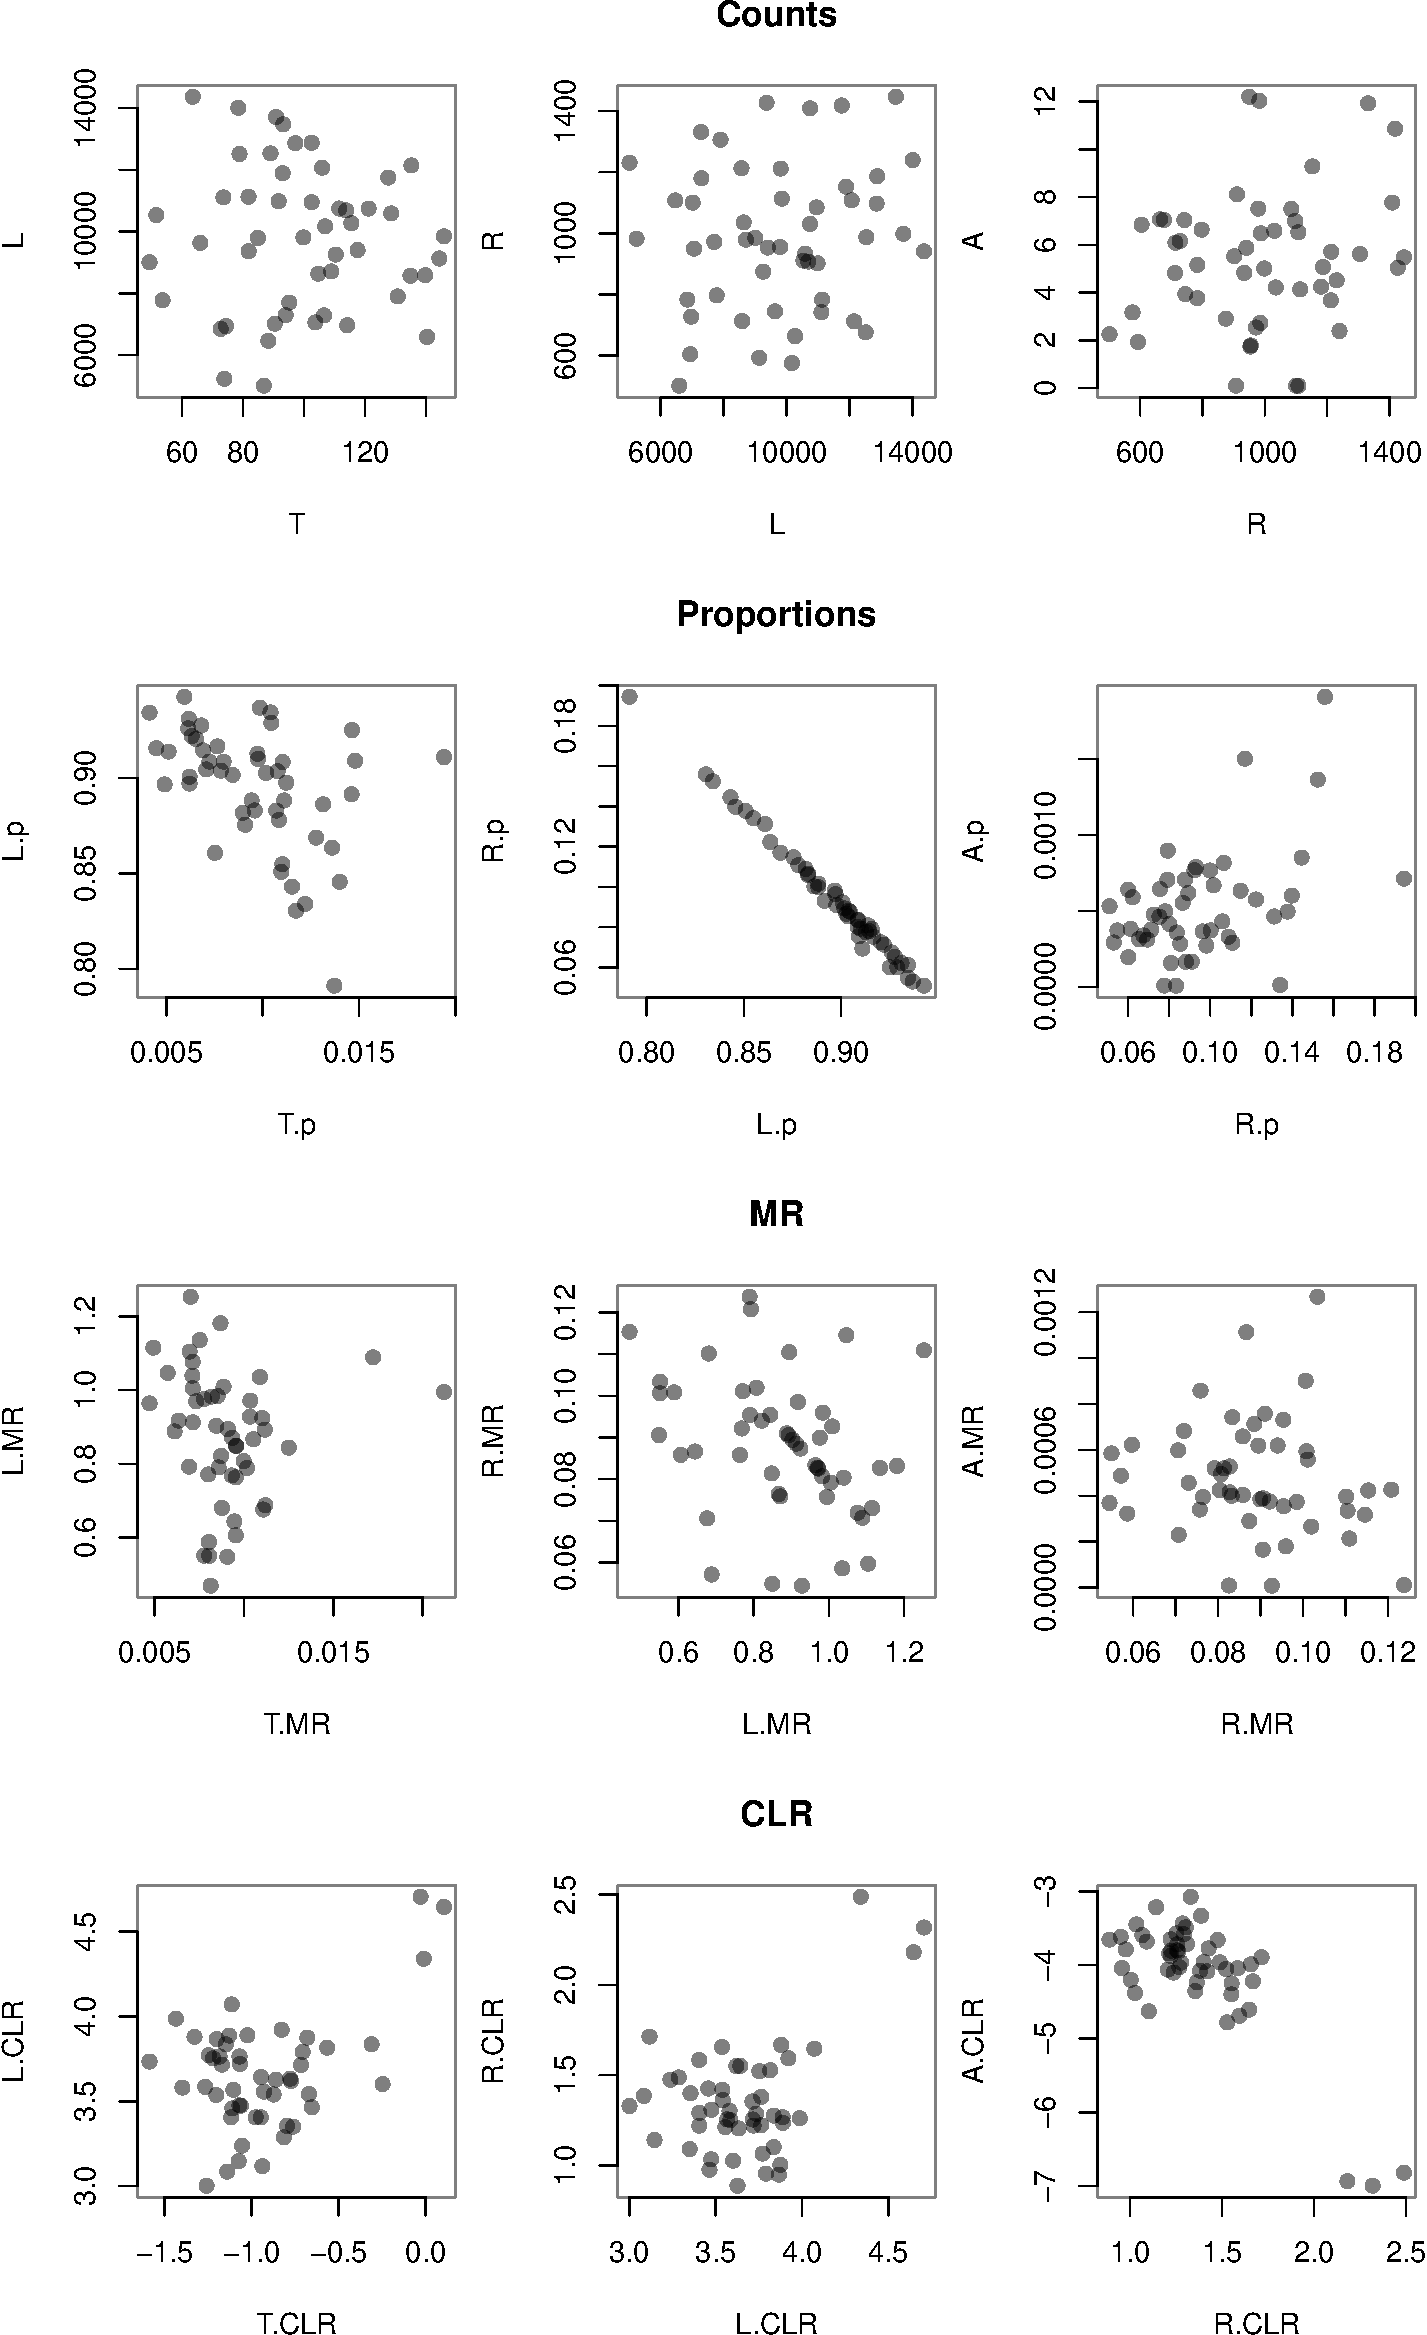
\includegraphics{_main_files/figure-latex/r-random-1.pdf}
\caption{\label{fig:r-random}Scatter plots of Ladybugs (L) vs.~Tigers (T),
Rabbits (R) vs.~Ladybugs and Aliens (A) vs.~Rabbits for simulated random
Normal data. Plots are shown for the actual count data, for the
proportional data, and for the proportional data after the MR or CLR
transformation.}
\end{figure}

The second row in Figure \ref{fig:r-random} shows the same pairs of
features in the same data after being converted to proportions: note
that this is exactly comparable to sequencing and being constrained by
an arbitrary sum as discussed in Chapter 5. Here we see that the the
proportional data have a radically different internal structure. The two
most relatively abundant features, R and L, which are uncorrelated in
the actual data are now almost perfectly negatively correlated as
proportions, R.p vs L.p. This is because the proportional data are now
not real numbers, but are instead are constrained by the arbitrary sum
of 1: \emph{the data are now compositional data}.

Recall from Figure \ref{fig:transformations} that the MR and CLR
transformations \emph{appeared} to restore most of the underlying
structure to the data. Using this simplified dataset, we can see that
this was an illusion. The MR transformation shown in row 3 of Figure
\ref{fig:r-random} seems to fix the problem caused by converting the
data from numbers to proportions since the points are more spread out.
However, closer inspection shows that this is not the case: compare L.MR
vs T.MR in row 3 with L vs T in row 1. It should be clear that the MR
transformation simply \emph{spreads the points out} without restoring
the actual structure of the underlying count data. This is unfortunate
and misleading since the stated purpose of the MR transformation is to
recover the underlying count structure of the environmental sample after
sequencing {[}REFS{]}. In the absence of a solid theoretical foundation,
it is difficult to say exactly how we should interpret these
MR-transformed data. The above MR plots were generated on the
proportional dataset, however only the scale of the \emph{MR} axes would
change if the MR normalization was conducted on the original numerical
data. Thus, conclusions derived from data that are MR-normalized
actually tell us little about the underlying counts from
enviroment---\emph{despite the pervasive use of this, and related, transformations in the biomedical literature}.

The last row in Fig \ref{fig:r-random} shows the proportional data
transformed by the clr transformation. Again, we see that the
transformed data are not similar to the actual count data. Thus,
conclusions made on clr-transformed data also cannot be directly related
to the count values of the actual dataset. So at this point we have a
conundrum: no transformation on post-sequencing data recapitulates the
pre-sequencing data that we want to examine.

\hypertarget{the-clr-transform-contains-relative-information}{%
\section{The CLR transform contains relative
information}\label{the-clr-transform-contains-relative-information}}

We are now in a position to realize that recovering the actual counts in
the environment from the post-sequencing data is impossible without
additional information. Some advocate the use of a spike-in of known
numbers of a molecule that can be used to normalize. However, in
practice one would need to include a sufficient number of these
molecules so that the random sampling error was very small, thus
decreasing the sequencing depth of the molecules being measured in the
experiment. In addition, practical examination of spike-in experiments
indicates that there is considerable variation in the spike-in molecules
that is attributed to batch effects {[}BARTON{]}, making their use
suspect.

Two transforms, the MR and clr transforms come closest to recapitulating
the overall shape of the univariate data as shown in Figure
\ref{fig:transformations}, and so appear to be promising. However, both
transformations (and all others) fail to recapitulate the multivariate
nature of the data as shown in Figure \ref{fig:r-random}. There is a way
forward as long as we are willing to change our point of view from
absolute numbers to relative values.

Interestingly, both the MR transform and the clr transform are based on
ratios. These tranforms share the insight that we need to examine the
abundance of a feature relative to the abundance of some other feature
or group of features. The MR transform uses as the reference a median
value calculated as in Equation \ref{eq:MR}. Two aspects of this
normalization are troubling. First, that the midpoint feature chosen as
the reference is likely different for each sample. Second, that the
values are scaled and interpreted as counts, even though the transformed
values are now ratios. Third, that the transformed values will be
different if the features have a different scale; i.e., if the features
are multiplied by a constant.

In contrast, the clr tranform has a firm theoretical foundation based on
compositional data analysis (Aitchison
\protect\hyperlink{ref-Aitchison:1986}{1986}). Data transformed by the
clr are the same whether they are counts, or proportions or are
multiplied by an arbitrary constant: they are what is called `scale
invariant'. We can demonstrate that the clr tranform provides the same
relative information on the actual count data by transforming the count
data, or the proportion data by the clr and plotting the result as shown
in Figure \ref{fig:r-ratios}. Further, clr-transformed data are
explicitly interpreted as the ratio between the count (or proportion) of
a feature and the geometric mean count (or proportion) of all features.
We can further modify the clr tranformation to use only those features
that have particular properties (such as non-0, low variance, etc) in
all samples {[}JIA{]} to avoid including features with a count of 0 in
the denominator. However, in this case we must keep in mind to interpret
the transformed values as the ratio between the feature and the
denominator.

\begin{figure}
\centering
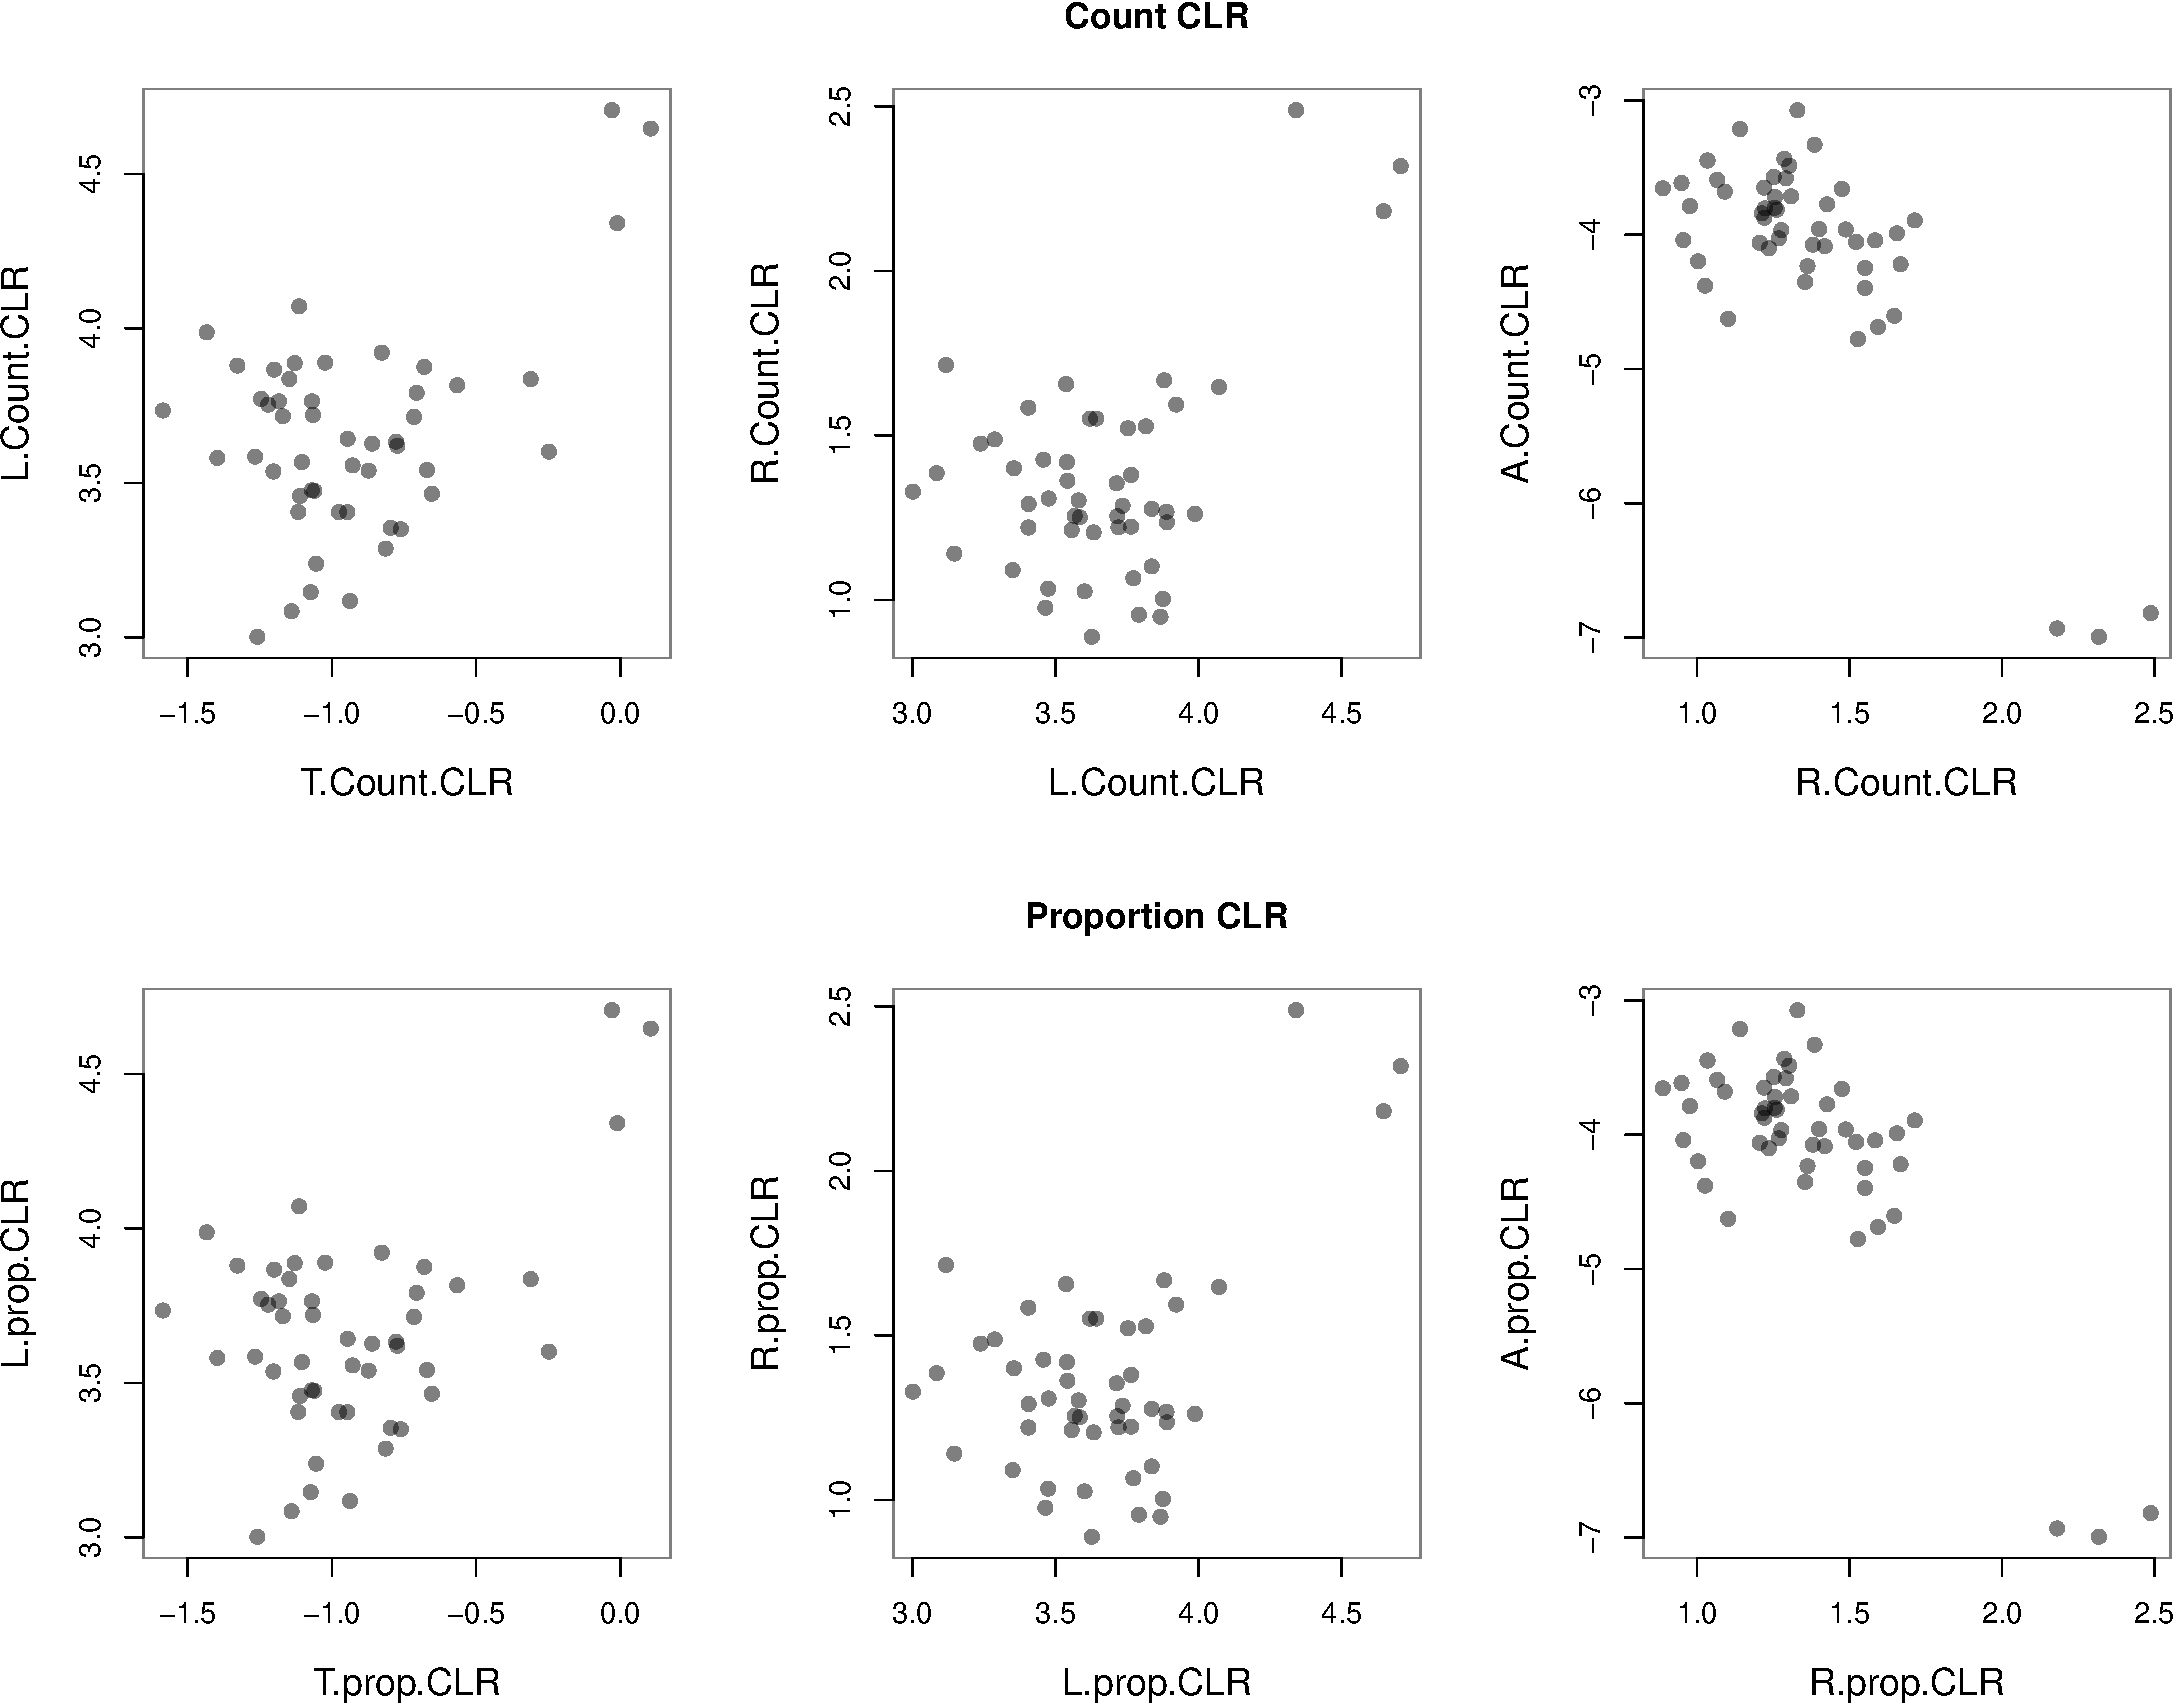
\includegraphics{_main_files/figure-latex/r-ratios-1.pdf}
\caption{\label{fig:r-ratios}\label{R_random} Plot of Ladybugs vs.~Tigers,
Rabbits vs.~Ladybugs and Aliens vs.~Rabbits for simulated random Normal
data after the MR normalization (top row). Plot of input numerical and
MR normalized data for Tigers, Ladybugs and Rabbits (bottom row)}
\end{figure}

\hypertarget{distances}{%
\chapter{Distances in high throughput sequencing}\label{distances}}

\hypertarget{distance-or-dissimilarity-metrics}{%
\section{Distance or dissimilarity
metrics}\label{distance-or-dissimilarity-metrics}}

The microbiome and transcriptome literature are replete with distance
metrics, and it is common to find that a single study will use several
distance metrics to report their findings. This is a problem since it
suggests that practitioners are unsure of the reason to use a metric;
consequently, the use of more than one metric leads to data dredging and
research degrees of freedom---both of which increase the chances of
finding false positives in the data to a surety.

\begin{figure}
\centering
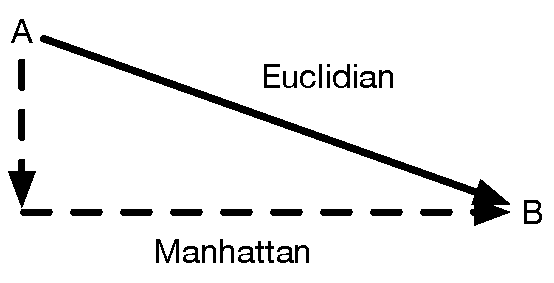
\includegraphics{./figs/distance.pdf}
\caption{Two primary distance metrics are Euclidian and Manhattan.
Euclidian distance is simply the straight-line distance between two
points, A and B. Manhattan distance, also called city block distance, is
the distance parallel to the axes of the co-ordinate system. Many other
distances are in use, but these two and their derivatives are the most
widespread.}
\end{figure}

Distance metrics can be broadly divided into those that require
partitioning and those that do not. The UniFrac (Lozupone et al.
\protect\hyperlink{ref-Lozupone:2011aa}{2011}; Lozupone and Knight
\protect\hyperlink{ref-unifrac:2005}{2005}) and philr (Silverman et al.
\protect\hyperlink{ref-Silverman:2017aa}{2017}) both require a
phylogenetic tree, making these metrics applicable only to situations
where the features can be so partitioned. For example, these distances
are useful when examining 16S rRNA gene sequencing experiments. We have
found that the unweighted UniFrac method is unreliable, and should be
used with caution {[}Wong, Wu, and Gloor
(\protect\hyperlink{ref-Wong:2016aa}{2016})\}, a point that was made in
the original UniFrac paper and subsequently forgotten. The philr metric
is a drop-in replacement for the weighted UniFrac distance metric and
should be used whenever possible, since \texttt{philr} is an ilr
transformation of the data where the sequential binary partitions are
made along the phylogenetic tree. The \texttt{philr} transformation is
thus compositionally appropriate. In practice, the weighted UniFrac
distance metric provides similar results to the Aitchison distance,
described below, and the ilr distance calculated using the philr
transform approaches the Aitchison distance when the number of features
is large.

Several non-phylogenetic distances are in widespread use in the
literature, and since the phylogenetic (or partitioning) distances are
difficult to apply to RNA-seq data, we will not illustrate these.
Non-phylogenetic distance metrics will be discussed in turn below, and
their effects on distances between a random samples illustrated.

\hypertarget{distances-in-counts-and-proportion}{%
\subsection{Distances in counts and
proportion\}}\label{distances-in-counts-and-proportion}}

Ideally, we use distance metrics to inform us as to something of
relevance in the actual sample. That is, if we collect our data on the
numbers of tigers, ladybugs, Rabbits and space aliens, what can we infer
about the actual data \emph{after  sequencing}? which as we have seen,
is the same as asking what can we infer after converting the data to
relative abundances (proportions)?

There are two main ways to think about distances: Euclidian and
Manhattan. The Euclidian distance is the straight-line distance between
two points. If we have a rectangular room, the Euclidian distance
between two corners would be the distance travelled by walking
diagonally across the room from one corner to the other. The Manhattan
distance would be the distance travelled by walking along the walls
between the two corners. Obviously, the Manhattan distance will always
be larger than the Euclidian distance. So how do these two simple
metrics, and others derived from them, compare when calculate on numbers
and on compositions?

In an ideal world when dealing with compositions, we would like a
distance metric that gives us an interpretable and stable measure of
distance between samples. Distances between samples should be:

\begin{itemize}
\tightlist
\item
  scale invariant (S): that is the distance between samples should not
  differ if we use proportions or percentages (or any other
  denominator).
\item
  subcompositional dominant (D): that is the distance between samples
  that contain all the features should be equal to or greater than the
  distance between the samples when one or more features are removed.
\item
  perturbation invariant (P): that is the distance between samples
  should be unchanged if we translate or rotate them in space.
\end{itemize}

Martin-Fernandes (\protect\hyperlink{ref-martin1998measures}{1998})
provide a very simple test that can be used to determine if a distance
metric is compositionally appropriate. We start with four samples, x1 to
x4 that contain three features each, and measure the distance between
the samples following a perturbation, or following feature subsetting.
The perturbed samples are labeled p1 to p4, and the subset samples
containing only the first two features are called s1 to s4.

\begin{Shaded}
\begin{Highlighting}[]
\NormalTok{x1 <-}\StringTok{ }\KeywordTok{c}\NormalTok{(}\DecValTok{1}\NormalTok{,}\DecValTok{2}\NormalTok{,}\DecValTok{7}\NormalTok{) }\OperatorTok{*}\StringTok{ }\FloatTok{0.1}
\NormalTok{x2 <-}\StringTok{ }\KeywordTok{c}\NormalTok{(}\DecValTok{2}\NormalTok{,}\DecValTok{1}\NormalTok{,}\DecValTok{7}\NormalTok{) }\OperatorTok{*}\StringTok{ }\FloatTok{0.1}
\NormalTok{x3 <-}\StringTok{ }\KeywordTok{c}\NormalTok{(}\DecValTok{3}\NormalTok{,}\DecValTok{4}\NormalTok{,}\DecValTok{3}\NormalTok{) }\OperatorTok{*}\StringTok{ }\FloatTok{0.1}
\NormalTok{x4 <-}\StringTok{ }\KeywordTok{c}\NormalTok{(}\DecValTok{4}\NormalTok{,}\DecValTok{3}\NormalTok{,}\DecValTok{3}\NormalTok{) }\OperatorTok{*}\StringTok{ }\FloatTok{0.1}

\NormalTok{x <-}\StringTok{ }\KeywordTok{rbind}\NormalTok{(x1,x2,x3,x4)}

\NormalTok{s <-}\StringTok{ }\KeywordTok{apply}\NormalTok{(x[,}\DecValTok{1}\OperatorTok{:}\DecValTok{2}\NormalTok{], }\DecValTok{1}\NormalTok{, }\ControlFlowTok{function}\NormalTok{(x) x}\OperatorTok{/}\KeywordTok{sum}\NormalTok{(x))}
\NormalTok{s <-}\StringTok{ }\KeywordTok{rbind}\NormalTok{(s,}\KeywordTok{c}\NormalTok{(}\DecValTok{0}\NormalTok{,}\DecValTok{0}\NormalTok{,}\DecValTok{0}\NormalTok{,}\DecValTok{0}\NormalTok{))}

\NormalTok{x.p <-}\StringTok{ }\KeywordTok{t}\NormalTok{( }\KeywordTok{t}\NormalTok{(x) }\OperatorTok{*}\StringTok{ }\KeywordTok{c}\NormalTok{(}\DecValTok{8}\NormalTok{,}\DecValTok{1}\NormalTok{,}\DecValTok{1}\NormalTok{) ) }\CommentTok{# perturbation, samples by row}

\NormalTok{p <-}\StringTok{ }\KeywordTok{t}\NormalTok{(}\KeywordTok{apply}\NormalTok{(x.p, }\DecValTok{1}\NormalTok{, }\ControlFlowTok{function}\NormalTok{(z) z}\OperatorTok{/}\KeywordTok{sum}\NormalTok{(z)))}
\end{Highlighting}
\end{Shaded}

This dataset is constructed so that the x1:x2 distance is greater than
the x3:x4 distance (Martín-Fernández et al.
\protect\hyperlink{ref-martin1998measures}{1998}). This is a bit
counterintuitive when examining the vectors since in both, the only
difference is in the first two features, and so these features determine
the distance. In both cases the two first features differ by 0.1, and so
if we treat these as non-compositional data we would infer that the
x1:x2 distance is equal to the x3:x4 distance. However, since the data
are compositional we must interpret the relative values: the first
feature in x1 is 0.5 that of the first feature in x2 whereas the first
feature in x3 is x4 is 0.75 that of the first feature in x4. The second
feature is the inverse relative difference. Thus, since the fold
difference between the first two features of x1 and x2 are larger than
the fold difference between the first two features of x3 and x4, the
distances between the pairs of samples must be correspondingly
different. When dealing with the subcomposition, the distances are
unchanged, because the ratios between the first two features is
unchanged, we have only dropped the non-informative last feature.

The relationships between the full composition and the subcomposition
can be observed in Figure \ref{fig:R-disttest}. The perturbed dataset is
simply a translation of the data on the simplex and should not change
the distance between samples. The ternary plot shows that our visual
intuition breaks down when examining data on a simplex because the
features are not linearly different in a composition. It is helpful to
think that a simplex is akin to a distorted map projection where we are
trying to show the relationships between the continents on a globe but
projected onto a flat map.

\begin{figure}

{\centering 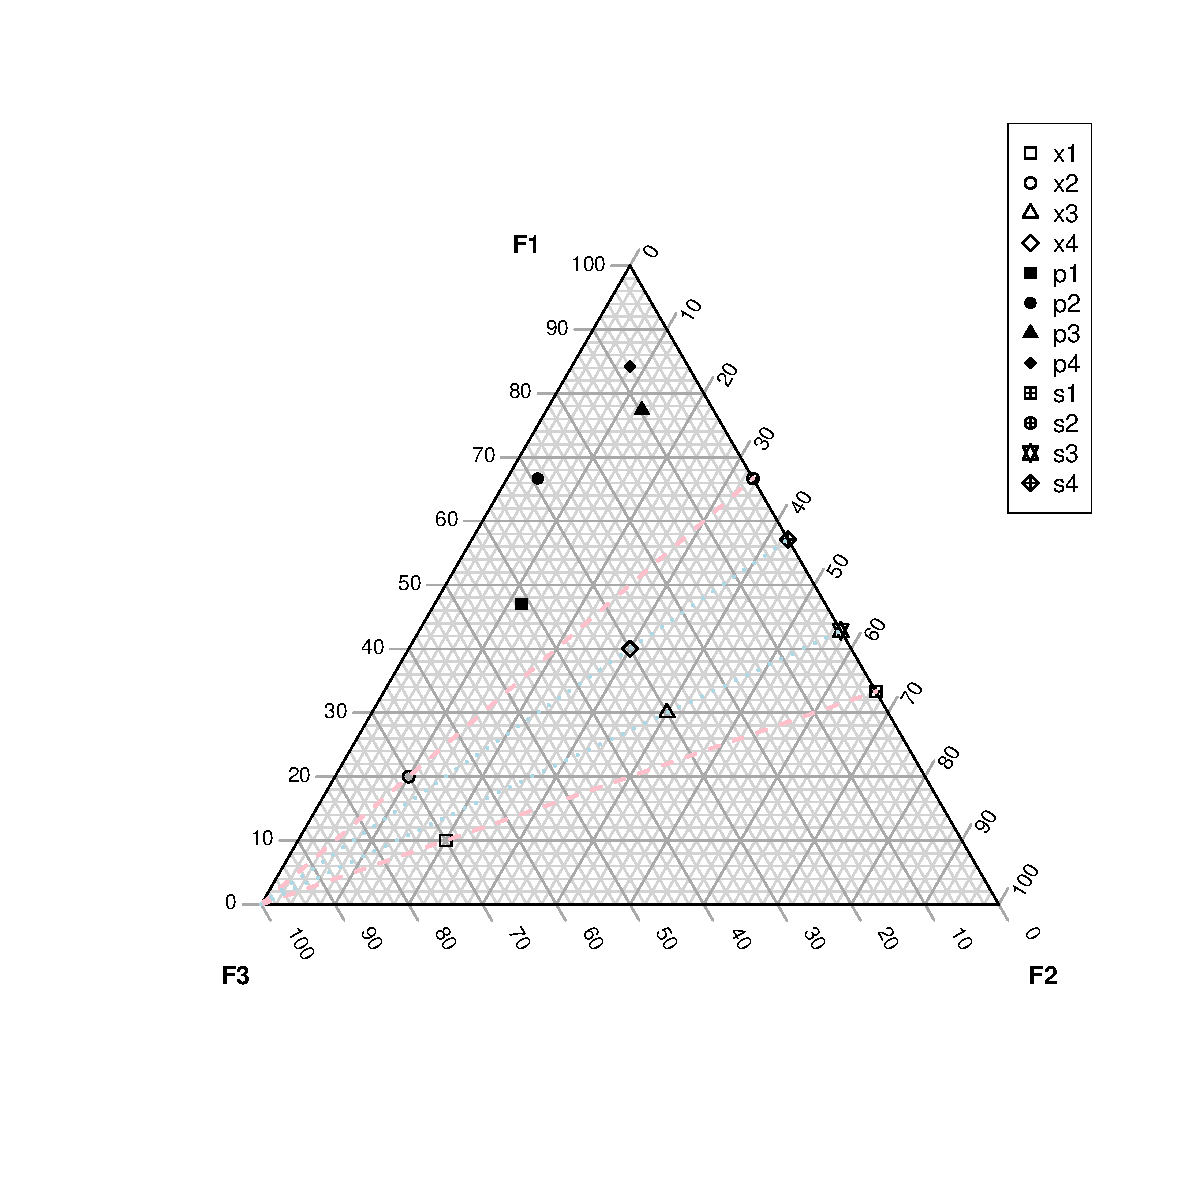
\includegraphics[width=0.7\linewidth]{_main_files/figure-latex/R-disttest-1} 

}

\caption{Ternary plot of toy data showing compositional properties. The simplex is the natural space of proportional data, or equivalently, probabilistic data, and contains one fewer dimension than does the data. The location of the four samples on the simplex are shown, along with their location after perturbation. The proportion of each feature in each sample determines the location of the feature on the simplex plot. The proportion of 1 is at the vertex with the label for each feature. The pink dashed line shows the projection of the data onto the F1-F2 proportion when feature 3 (F3) is removed. Distances on the simplex are not necessarily intuitive, since the x1, x2 distance is about twice that of the x3, x4 distance, although on the plot the distances appear similar. This is because distances are non-linear and become more distorted as the margin of the plot is approached: see [@martin1998measures] for an explanation of this.}\label{fig:R-disttest}
\end{figure}

\begin{table}[!h]
\caption{Distance metrics on the simplex. The x1,x2 distance should be larger than the x3,x4 distance, the distance should be the same if we change the scale (S), the perturbation should not change the distances since it is simply a translation (P), and the distance between sample subcompositions should be no larger than the full composition (D). Among the distances compared, only the Aitchison distance---the Euclidian distance of the clr values---fulfills these properties. }\vspace{0.2cm}
\centering
\resizebox{\columnwidth}{!}{%
\begin{tabular}{l r r r r r r}
\hline
Metric (SDP) & d(x1,x2) & d(p1,p2) & d(s1,s2) & d(x3,x4) & d(p3,p4) & d(s3,s4) \\ \hline \hline
Euclidian (---) & 0.14 & 0.24 & 0.47 & 0.14 & 0.09 & 0.20\\
Manhattan (---) & 0.20 & 0.40 & 0.67 & 0.20 & 0.14 & 0.29\\
Bray-Curtis (S--) & 0.10 & 0.20 & 0.33 & 0.10 & 0.06 & 0.14\\
JSD (SD-)& 0.13 & 0.15 & 0.13 & 0.08 & 0.06 & 0.08\\
Aitchison (SDP) & 0.98 & 0.98 & 0.98 & 0.41 & 0.41 & 0.41\\ \hline
\end{tabular}
}
\label{tab:metrics}
\end{table}

Table \ref{tab:metrics} shows the properties of several distance metrics
on the synthetic vectors. By definition, the Euclidian and Manhattan
distances are not scale invariant, perturbation invariant, nor are they
subompositionally dominant. These metrics should \emph{never} be used
for proportional (compositional) data. The Bray-Curtis dissimilarity (or
if symmetrized Bray-Curtis distance) is scale invariant by definition
since all values are scaled between 0 and 1. However, the Bray-Curtis
dissimilarity is not subcompositionally dominant, nor is it perturbation
invariant. Thus, the Bray-Curtis metric will be sensitive to the choice
of features that are included in the analysis, and raw and normalized
data are expected to give different results.

The Jensen-Shannon Distance is a symmetrized version of the
Kulback-Leibler divergence metric that is widely used when comparing
probability vectors {[}REF, REF{]}. This metric is both scale invariant
and subcompositionally dominant. Thus, the JSD would be expected to give
results consistent with the whole when used on subsets of the data.
However, the JSD metric is not perturbation invariant, and so will not
give the same results on the raw and transformed data.

The Aitchison distance is the Euclidian distance calculated on the
log-ratio transformed data; here we use the clr transform. The Aitchison
distance fulfills all properties and so is expected to give consistent
results when a dataset is subsetted, when the dataset is scaled, or when
the dataset is transformed. Thus, this distance metric should be used
whenever possible. The utility of the distance metrics are illustrated
more fully below.

\hypertarget{graphical-demonstration-of-distance-pathologies}{%
\section{Graphical demonstration of distance
pathologies}\label{graphical-demonstration-of-distance-pathologies}}

I return now to the simple the Ladybugs (L), Tigers (T), Rabbits (R),
and Aliens (A) dataset and examine the distance between samples using
different metrics. Recall that we desire to find a distance metric that
when used on the compositional data obtained after sequencing tells us
something about the count data from the environment before sequencing.
Thus, we should obtain a linear relationship between the count and
compositional data if the distance metric is generally useful, and we
compare the counts to both simple proportions and proportions after the
DM transformation for all distance metrics.

We first examine the simple Euclidian and Manhattan distances.

\begin{figure}

{\centering 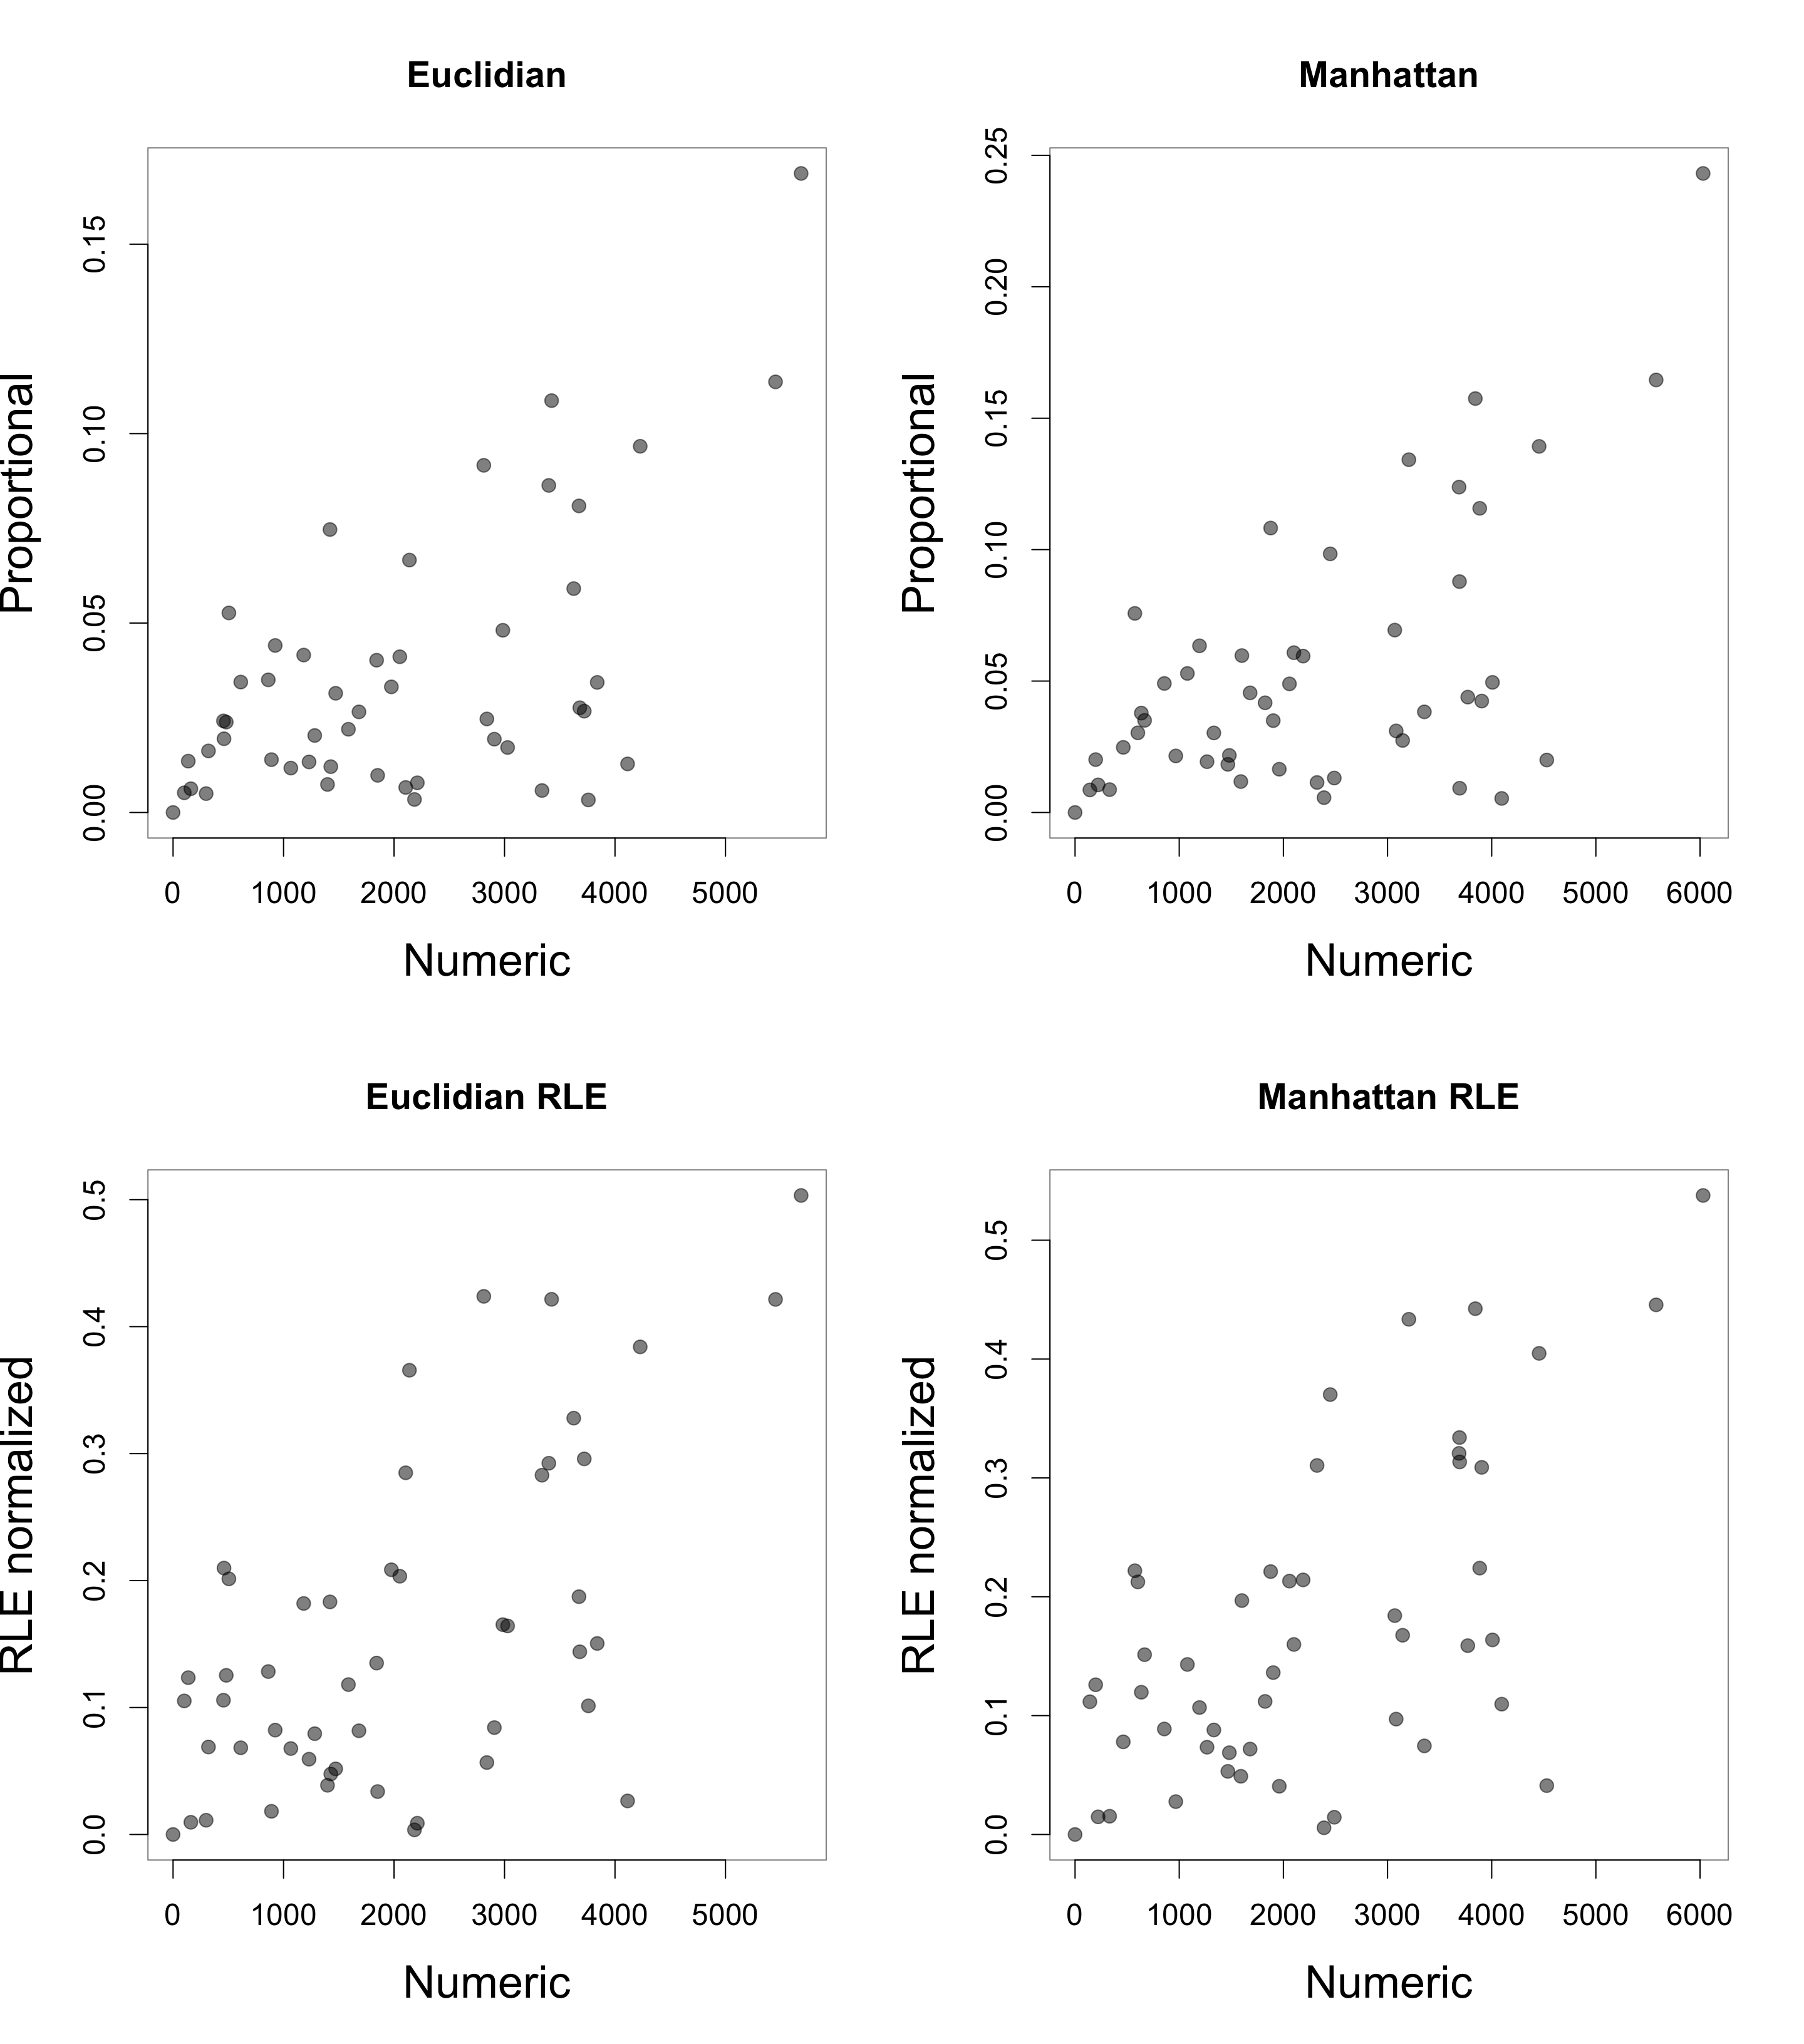
\includegraphics[width=0.8\linewidth]{_main_files/figure-latex/R-block-dist-1} 

}

\caption{Scatter plot of the distances computed on numeric, proportional and DM-normalized data. The X-axis has the distances computed on the original numeric data, and the Y-axis has the distances computed on the same data converted to proportions, or when the proportions are count-normalized using the DM normalization. The distances for the count data and the proportions or the DM normalized data are obviously not linearly related.}\label{fig:R-block-dist}
\end{figure}

We can see that the Euclidian and Manhattan distances are generally
correlated, but not identical, when comparing distances in the original
set of random samples only, or when the data in the samples are
converted to proportions. However, the distances between samples are
very different when comparing the numerical and proportional data. This
tells us that the inferences we make from sequencing data can not
translate to inferences about the actual abundances of features in the
environment, but only to their relative abundances. So which distance
metric should we use for proportional data? It turns out that neither
are suitable because these distance metrics assume linear differences
between features, and this is not true in proportional data (Aitchison
\protect\hyperlink{ref-Aitchison:1986}{1986}).

Data normalizations are often touted as removing the compositionality of
the data. We shall see that this is not true, and inappropriate data
transformations confound, rather than providing clarity.

Plotting three of the possible combinations, we can see that the
features are essentially uncorrelated with each other and each sample is
a random distances from any other. Any inference we make from
transformations of this data must be relatable to this `ground truth'. I
now run through each of the transformations in turn, and illustrate the
difference between the actual data, and the transformed data.

\hypertarget{bray-curtis-dissimilarity}{%
\subsection{Bray-Curtis Dissimilarity}\label{bray-curtis-dissimilarity}}

The Bray-Curtis dissimilarity is a modified Manhattan distance
normalized to range between 0 and 1, thus the Manhattan distance and the
Bray-Curtis (BC) distances are essentially linearly related changing
only the scale of the measure. One quirk of the BC dissimilarity is that
it cannot be calculated if any of the values in the matrix are less
than, making it incompatible with logarithmic or log-ratio transformed
data.

\begin{figure}

{\centering 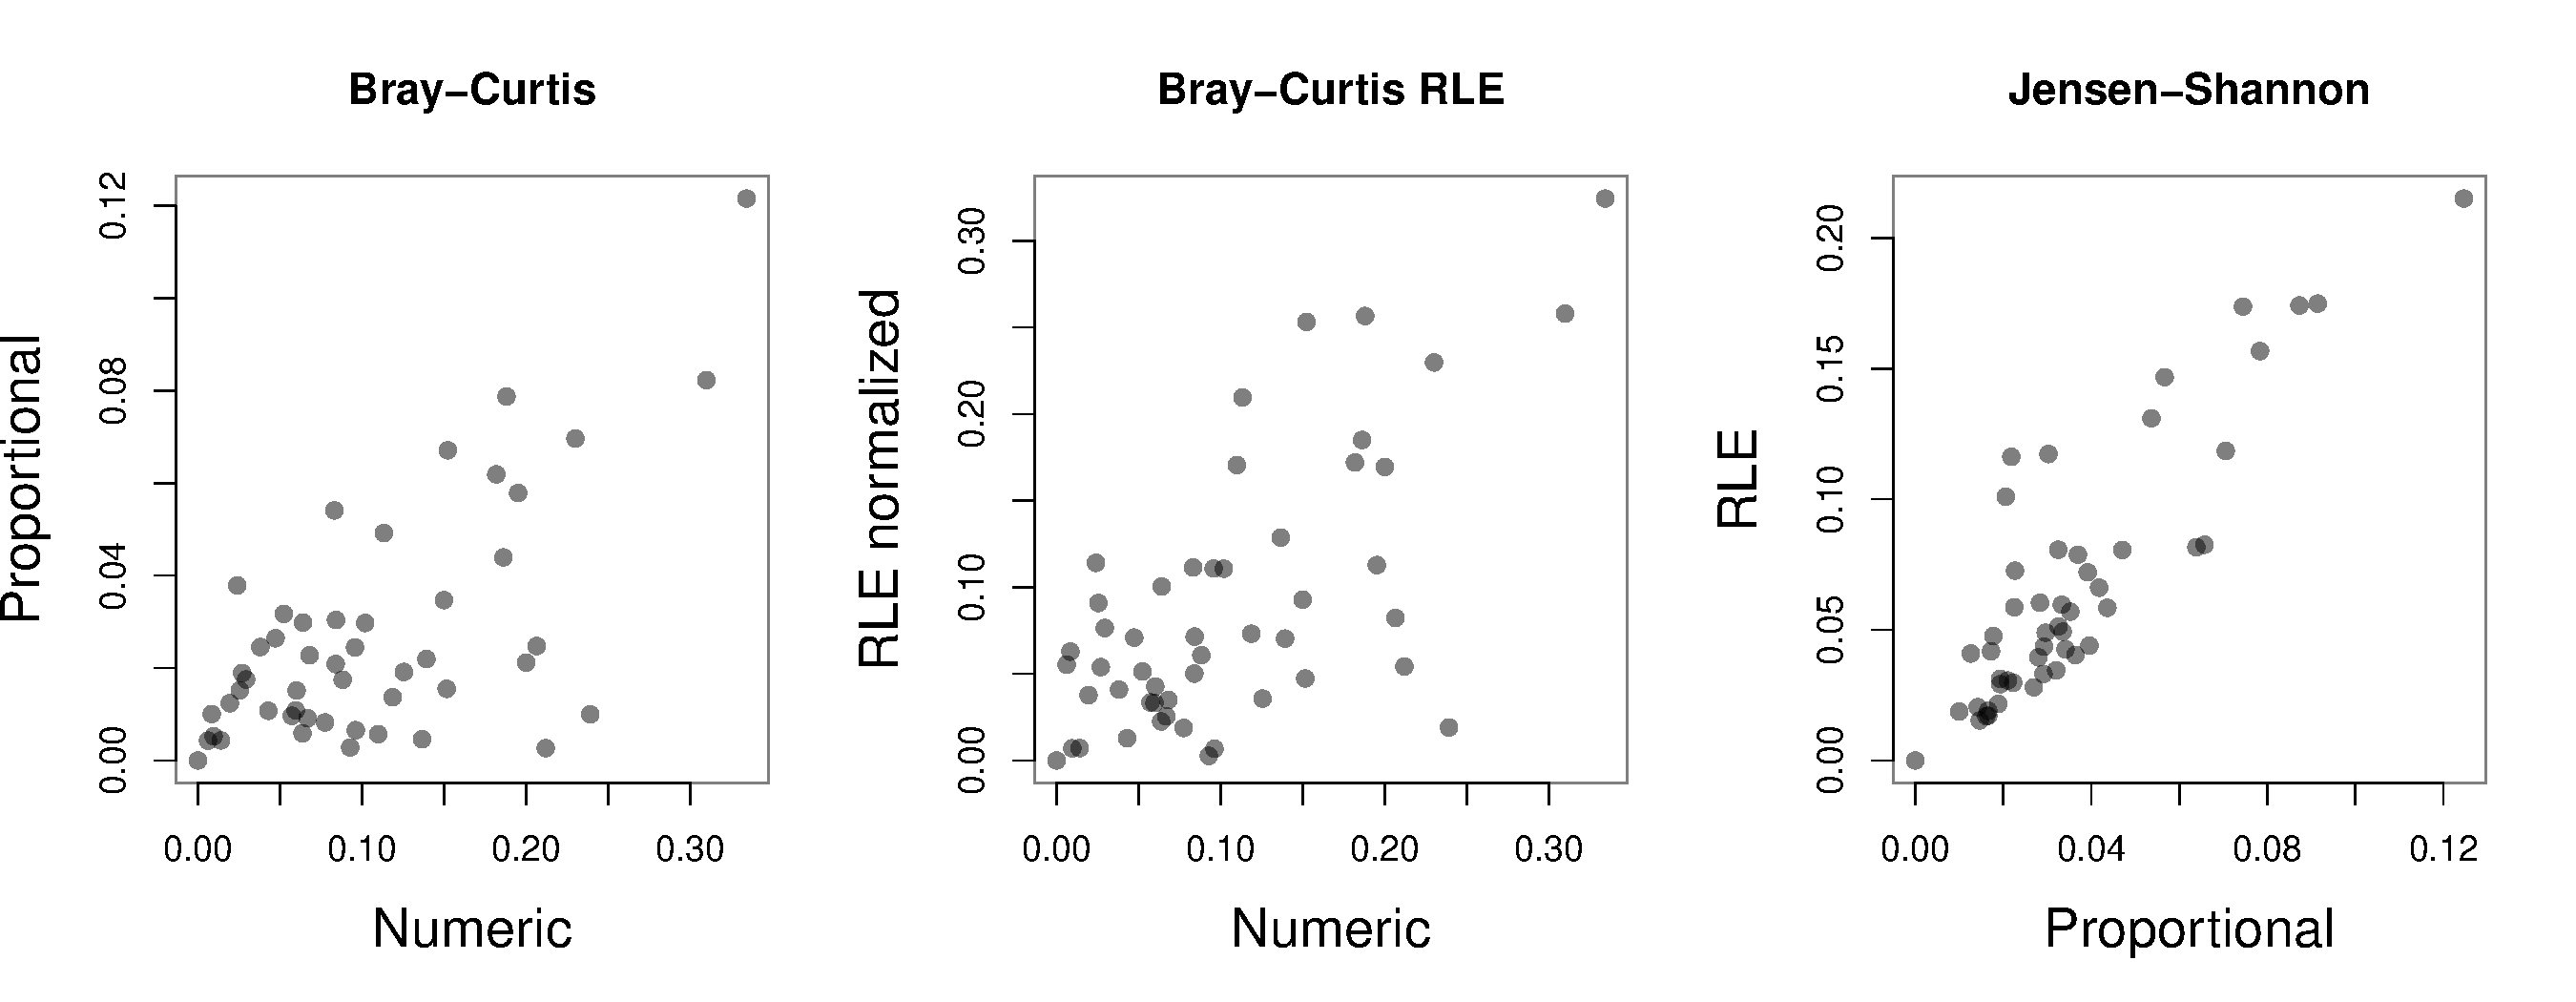
\includegraphics[width=0.8\linewidth]{_main_files/figure-latex/R-block-bray-1} 

}

\caption{Scatter plot of Bray-Curtis dissimilarities, or Jensen-Shannon divergence  of numerical vs. proportional and DM normalized data.}\label{fig:R-block-bray}
\end{figure}

\hypertarget{distances-of-clr-transformed-data}{%
\subsection{Distances of clr transformed
data}\label{distances-of-clr-transformed-data}}

The blah blah blah

\begin{figure}

{\centering 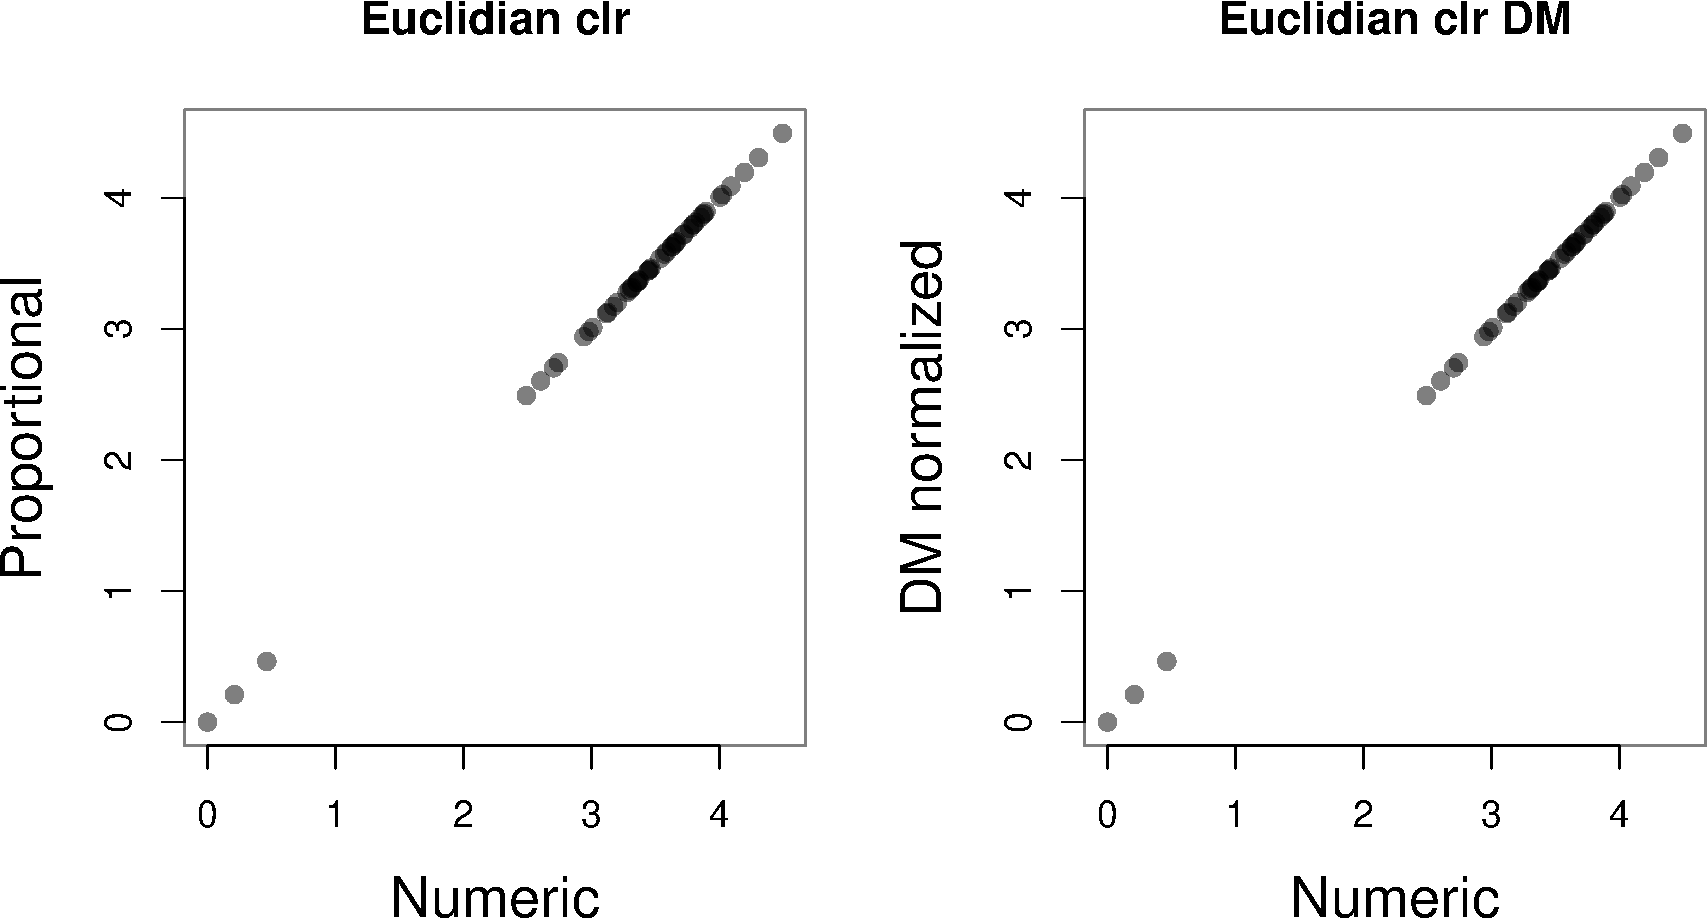
\includegraphics[width=0.8\linewidth]{_main_files/figure-latex/R-clr-plot-1} 

}

\caption{Scatter plot of Euclidian distances of the clr transformed numeric or proportional data. As above, DM indicates proportional data scaled by the DM normalization.}\label{fig:R-clr-plot}
\end{figure}

\texttt{plot\_ly(x=ran.dat[,"L"], y=ran.dat[,"T"], z=ran.dat[,"R"])}

\texttt{plot\_ly(x=ran.dat.prop[,"L"], y=ran.dat.prop[,"T"], z=ran.dat.prop[,"R"])}

\texttt{plot\_ly(x=ran.dat.DM[,"L"], y=ran.dat.DM[,"T"], z=ran.dat.DM[,"R"])}

\hypertarget{biplot}{%
\chapter{Exploring compositional data: the compositional
biplot}\label{biplot}}

There are three main data analysis issues that must be acknowledged.

First, the nature of these data are misunderstood. As outlined above,
the number of counts observed per OTU are determined entirely by the
capacity of the instrument and provide no information about the number
of molecules in the input sample. Recall that both bacterial growth, and
PCR are doubling processes and not linear processes, and so would be
better modelled as log\(_2\) differences.

Understanding that we are dealing with fold-change data is an explicit
acknowledgement that the data do not map to normal Euclidian space where
differences are linear. Commonly used statistical tests expect linear
differences between values and so are compromised to some degree, often
catastrophically(Aitchison
\protect\hyperlink{ref-Aitchison:1986}{1986},vandenBoogaart2008320)
Therefore, the often-used approaches of converting the OTU count values
to proportions or percentages and conducting statistical tests on those
values, or of using data reduction strategies such as Principle
Component Analysis on the values are inappropriate because the
differences between values are not linear. An alternative approach is to
convert the OTU counts to ratios(Aitchison
\protect\hyperlink{ref-Aitchison:1986}{1986}; Aitchison and J. Egozcue
\protect\hyperlink{ref-aitchison:2005}{2005}; Pawlowsky-Glahn and
Egozcue \protect\hyperlink{ref-Pawlowsky-Glahn:2006}{2006};
Pawlowsky-Glahn and Buccianti
\protect\hyperlink{ref-pawlowsky2011compositional}{2011}) which makes
the differences between the ratios of values linear, and so allows the
use of common statistical tests.

However the user must interpret the output as ratios between feature
abundances rather than absolute differences(Pawlowsky-Glahn and
Buccianti \protect\hyperlink{ref-pawlowsky2011compositional}{2011}) This
approach is described below.

Second, high throughput sequencing (HTS) data represent samples of an
unknown underlying large number of molecules. Thus, there is a large and
unappreciated error of estimation that is problematic when dealing with
these data(Fernandes et al.
\protect\hyperlink{ref-fernandes:2013}{2013}) The high error of
estimation often results in false positive identification of
differences, in fact, the statistical result can often be explained
entirely by sampling variation. This error is not captured by
rarefaction or even acknowledged by other normalization methods and
should be estimated and accounted for when deciding what is a
significant difference.

Third, 16S rRNA gene sequencing surveys, and similar experiments,
contain many variables in each sample. Thus, any analysis that attempts
to characterize the individual differences between groups must correct
for the many hypotheses that are being tested. This step is often
ignored, even in work published in very high profile journals subject to
rigorous peer review.

The purpose of these notes is to show why HTS data for 16S rRNA gene
sequencing, and any similar experiments such as RNA-seq, should be
treated as ratio data and that it is possible to do so simply. We show
that this approach accurately recapitulates the shape of the data for
both constrained and unconstrained datasets. We show that converting the
data to ratios can accurately model the very high variability at the low
count margins, and that rarefaction under-estimates this variability. We
use an example from the literature to show how ignoring these factors
leads to improper conclusions.

\hypertarget{analyzing-16s-rrna-gene-sequencing-experiments}{%
\chapter{Analyzing 16S rRNA gene sequencing
experiments}\label{analyzing-16s-rrna-gene-sequencing-experiments}}

The human microbiome project has initiated the large-scale
culture-independent analysis of microbial communities, and transcriptome
analysis has led to the study of the transcriptional response to many
different disease and ecological states.

However, many studies fail to replicate earlier studies even when the
same technologies and strategies are used. As just one example, a
multitude of studies have examined the link between autism and the human
gut microbiota. These have variously implicated x,y,\ldots{},and z
microbe as being linked to the condition. In a recent high-profile paper
by Hsiao et al. (\protect\hyperlink{ref-Hsiao:2013}{2013}),
\emph{Bacillus fragilis} was suggested to restore the gut microbiome of
a mouse autism model from `autistic-like' to `normal'. Examination of
the dataset shows that the conclusion was likely due to chance alone
(Gloor, Wu, et al. \protect\hyperlink{ref-gloor2016s}{2016}; Gloor and
Reid \protect\hyperlink{ref-Gloor:2016cjm}{2016}). While the autism
dataset serves as a facile example, the literature are replete with
other examples.

\hypertarget{oral}{%
\chapter{HMP oral microbiota exploration}\label{oral}}

\hspace{2cm}\begin{minipage}[ct]{10cm}
\parskip=5pt
\parindent=5pt
This example was first presented as part of the CoDa microbiome tutorial in Hinxton, UK in September 2016 at the Human-host microbe interactions conference. Dr. Jean Macklaim co-wrote and did trouble-shooting of this tutorial. It has been modified for clarity and completeness for this book.
\end{minipage}
\vspace{1cm}

We start the differential abundance analysis using a simple dataset
derived from the original HMP oral microbiota dataset. This dataset is
used because it is exceedingly sparse and so a good test of the method.

The first task is to read in the data and to generate the ALDEx2 output.
The data contains 187 attached keratinized gingeva (ak) and 186 outside
plaque (op) samples.

\begin{Shaded}
\begin{Highlighting}[]
\CommentTok{# The Basic ALDEx2 workflow for two conditions}

\CommentTok{# this has been modified to reduce the number of Dir monte-carlo instances}
\CommentTok{# I suggest generating sufficient Dir MCI to get at least 4000 when}
\CommentTok{# the product of the number of samples in the smallest group x DMCI}

\CommentTok{# this process can be slow, so I have pre-computed and saved the file}


\CommentTok{# read the dataset}
\NormalTok{d.subset <-}\StringTok{ }\KeywordTok{read.table}\NormalTok{(}\KeywordTok{paste}\NormalTok{(tutorial_data, }\StringTok{"ak_vs_op.txt"}\NormalTok{, }\DataTypeTok{sep=}\StringTok{""}\NormalTok{),}
    \DataTypeTok{row.names=}\DecValTok{1}\NormalTok{, }\DataTypeTok{header=}\NormalTok{T)}
\CommentTok{# make a vector containing the two names of the conditions}
\CommentTok{# in the same order as in the column names}
\NormalTok{d.conds <-}\StringTok{ }\KeywordTok{c}\NormalTok{(}\KeywordTok{rep}\NormalTok{(}\StringTok{"ak"}\NormalTok{, }\KeywordTok{length}\NormalTok{(}\KeywordTok{grep}\NormalTok{(}\StringTok{"ak"}\NormalTok{, }\KeywordTok{colnames}\NormalTok{(d.subset))) ),}
    \KeywordTok{rep}\NormalTok{(}\StringTok{"op"}\NormalTok{, }\KeywordTok{length}\NormalTok{(}\KeywordTok{grep}\NormalTok{(}\StringTok{"op"}\NormalTok{, }\KeywordTok{colnames}\NormalTok{(d.subset)))) )}
\CommentTok{# generate Monte-Carlo instances of the probability of observing each count}
\CommentTok{# given the actual read count and the observed read count.}
\CommentTok{# this returns a set of clr values, one for each MC instance, which}
\CommentTok{# constitutes a distribution of clr values}
\CommentTok{# note that the latest version of ALDEx2 requires conds explicitly}
\NormalTok{d.x <-}\StringTok{ }\KeywordTok{aldex.clr}\NormalTok{(d.subset, }\DataTypeTok{conds=}\NormalTok{d.conds, }\DataTypeTok{mc.samples=}\DecValTok{22}\NormalTok{)}
\CommentTok{# calculate effect sizes for each mc instance, report the expected value}
\NormalTok{d.eff <-}\StringTok{ }\KeywordTok{aldex.effect}\NormalTok{(d.x, d.conds, }\DataTypeTok{include.sample.summary=}\OtherTok{TRUE}\NormalTok{)}
\CommentTok{# perform parametric or non-parametric tests for difference}
\CommentTok{# report the expected value of the raw and BH-corrected P value}
\NormalTok{d.tt <-}\StringTok{ }\KeywordTok{aldex.ttest}\NormalTok{(d.x, d.conds)}
\CommentTok{# concatenate everything into one file}
\NormalTok{d.all <-}\StringTok{ }\KeywordTok{data.frame}\NormalTok{(d.eff,d.tt)}

\KeywordTok{write.table}\NormalTok{(d.all, }\DataTypeTok{file=}\KeywordTok{paste}\NormalTok{(tutorial_data, }\StringTok{"ak_vs_op_aldex.txt"}\NormalTok{, }\DataTypeTok{sep=}\StringTok{""}\NormalTok{), }\DataTypeTok{sep=}\StringTok{"}\CharTok{\textbackslash{}t}\StringTok{"}\NormalTok{,}
    \DataTypeTok{quote=}\OtherTok{FALSE}\NormalTok{, }\DataTypeTok{col.names=}\OtherTok{NA}\NormalTok{)}
\end{Highlighting}
\end{Shaded}

We display the results using a number of different plots in Figure
\ref{hmp_aldex_plot} to show how each plot gives a different way of
exploring the data.

The mainstay that we advocate is the effect plot (Gloor, Macklaim, and
Fernandes \protect\hyperlink{ref-Gloor:2015}{2016}), that plots the
constituents of normalized change, or effect size. The effect plot shows
the relationship between the between group difference and the
within-group dispersion for each feature. The Bland-Altman plot (Altman
and Bland \protect\hyperlink{ref-altman:1983}{1983}) shows the
relationship between the between group difference and the relative
abundance of each feature. The volcano plot (Cui and Churchill
\protect\hyperlink{ref-Cui:2003aa}{2003}) shows the relationship between
fold-change and the logarithm of the p-value. Finally, the effect
vs.~p-value plot shows the relationship between effect size and p-value.

\begin{figure}
\centering
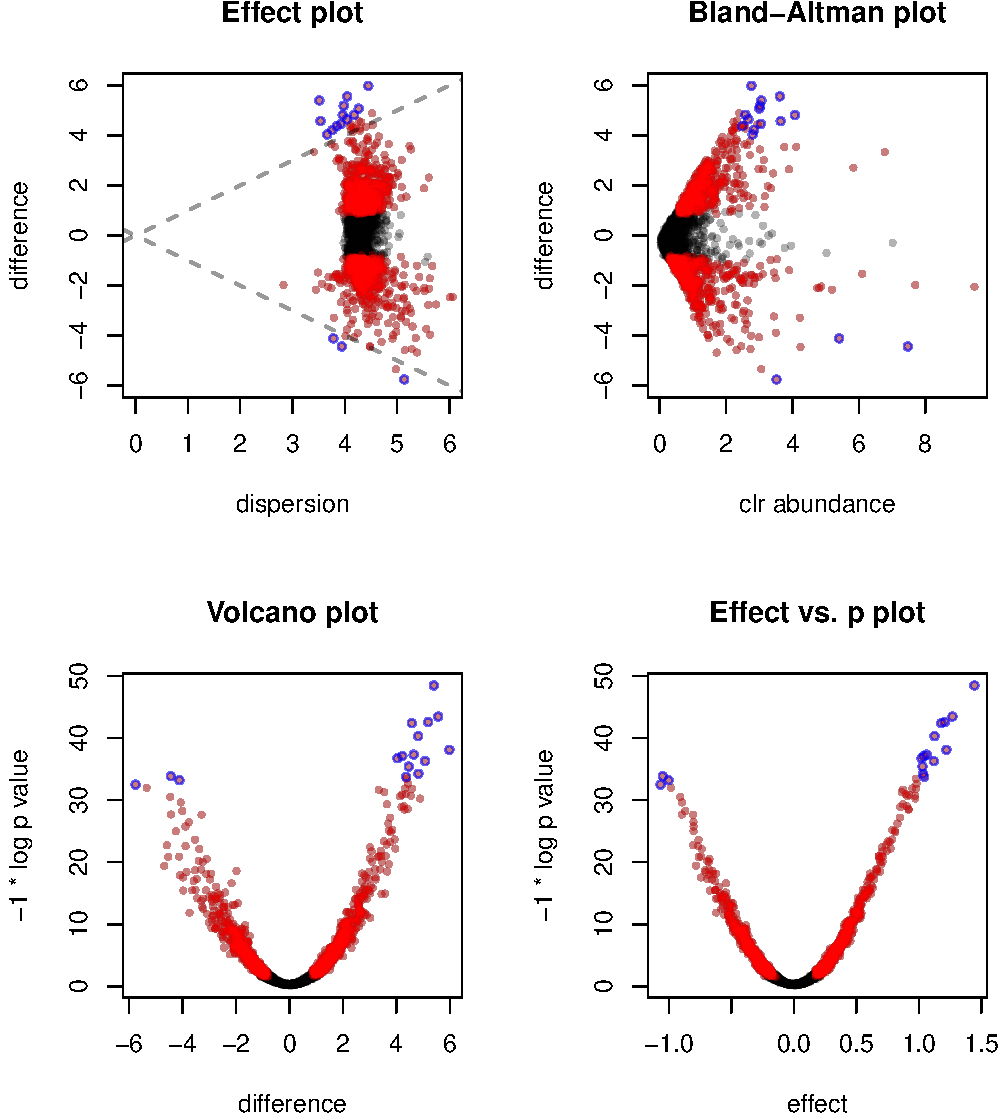
\includegraphics{_main_files/figure-latex/hmp_aldex_plot-1.pdf}
\caption{(\#fig:hmp\_aldex\_plot)Plotted here are taxa with no
difference between groups (grey), a statistically difference between
groups (red), and with an effect larger than 1 (blue circles). These are
plotted using different plots (described clockwise from top left). The
effect plot (Gloor, Macklaim, and Fernandes
\protect\hyperlink{ref-Gloor:2015}{2016}) illustrates the difference
between groups vs.~the dispersion (variance) within groups. If the
effect is greater than one (outside the grey lines), then, on average
the taxa are separable by eye when plotted; roughly, they would be seen
to have a greater difference than standard deviation. Effect is a more
robust measure of difference than are P values, since the latter depend
on sample size; large sample sizes will always give low P values (Halsey
et al. \protect\hyperlink{ref-Halsey:2015aa}{2015}). We can see this
here where the large sample size means that even highly variable OTUs
are significantly different. The Bland-Altman plot (Altman and Bland
\protect\hyperlink{ref-altman:1983}{1983}) compares difference and
abundance, and is often seen in RNA-Seq data. The Volcano plot (Cui and
Churchill \protect\hyperlink{ref-Cui:2003aa}{2003}) shows the
association between difference and P value, and the final plot shows the
association between effect and P value.}
\end{figure}

Let's get a visual idea what is meant by the effect size as used in
ALDEx2 using two significant features. OTU 3760 has an effect size of
1.04, ol 0.107, we.eBH 5.2e-31, wi.eBH 7.6e-38, and OTU 7805 is still
significant but has an effect size of about 0.25, ol 0.37, we.eBH
0.0055, wi.eBH 0.0002.

\begin{figure}
\centering
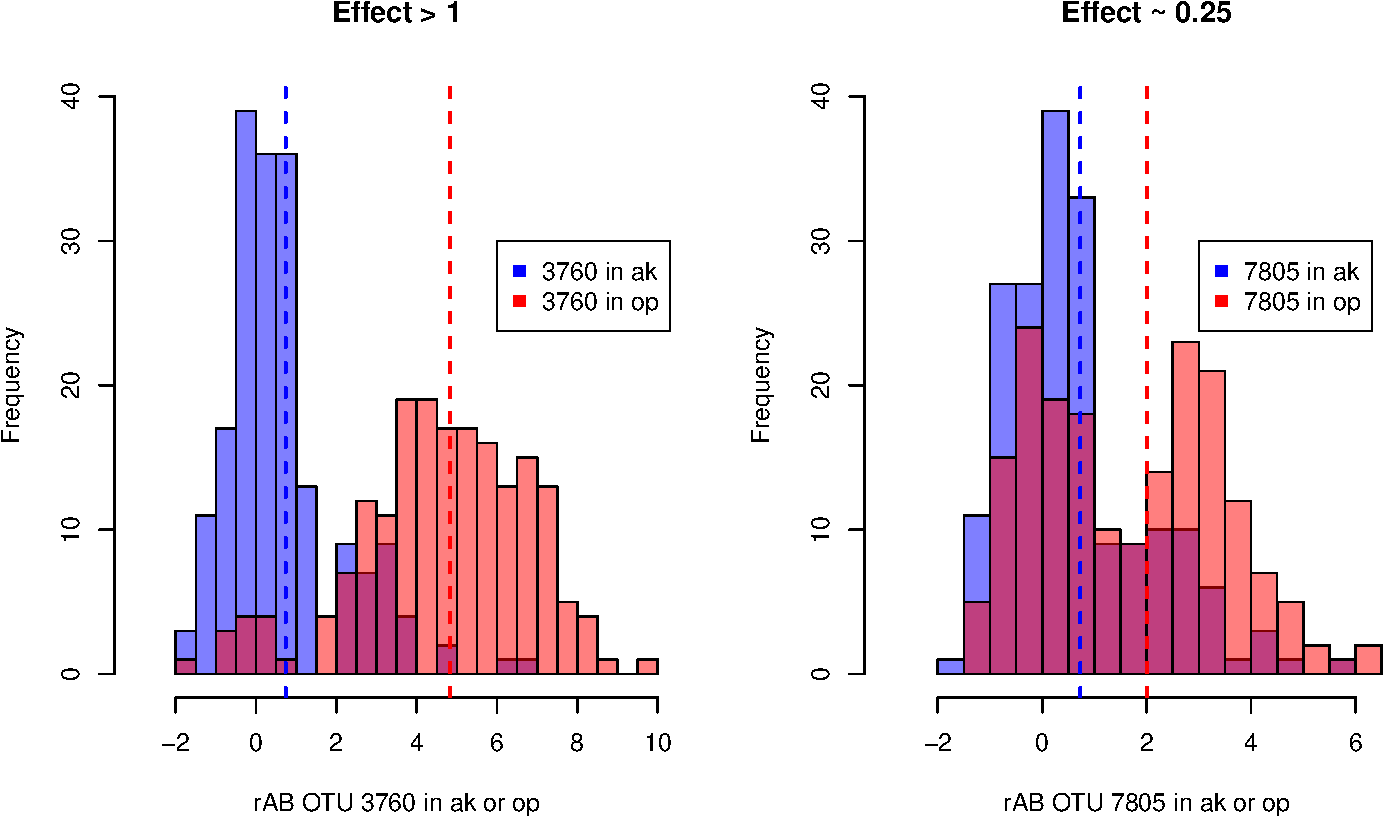
\includegraphics{_main_files/figure-latex/hmp_aldex_effect-1.pdf}
\caption{(\#fig:hmp\_aldex\_effect)Histograms showing the separation
between groups when choosing OTUs with large effect sizes (left), or
OTUs with small effect size (right). OTUs with the largest effect are
the `most reliably different' between groups, and should be chosen over
those that are `most significantly different' whenever possible.}
\end{figure}

\newpage

\begin{figure}
\centering
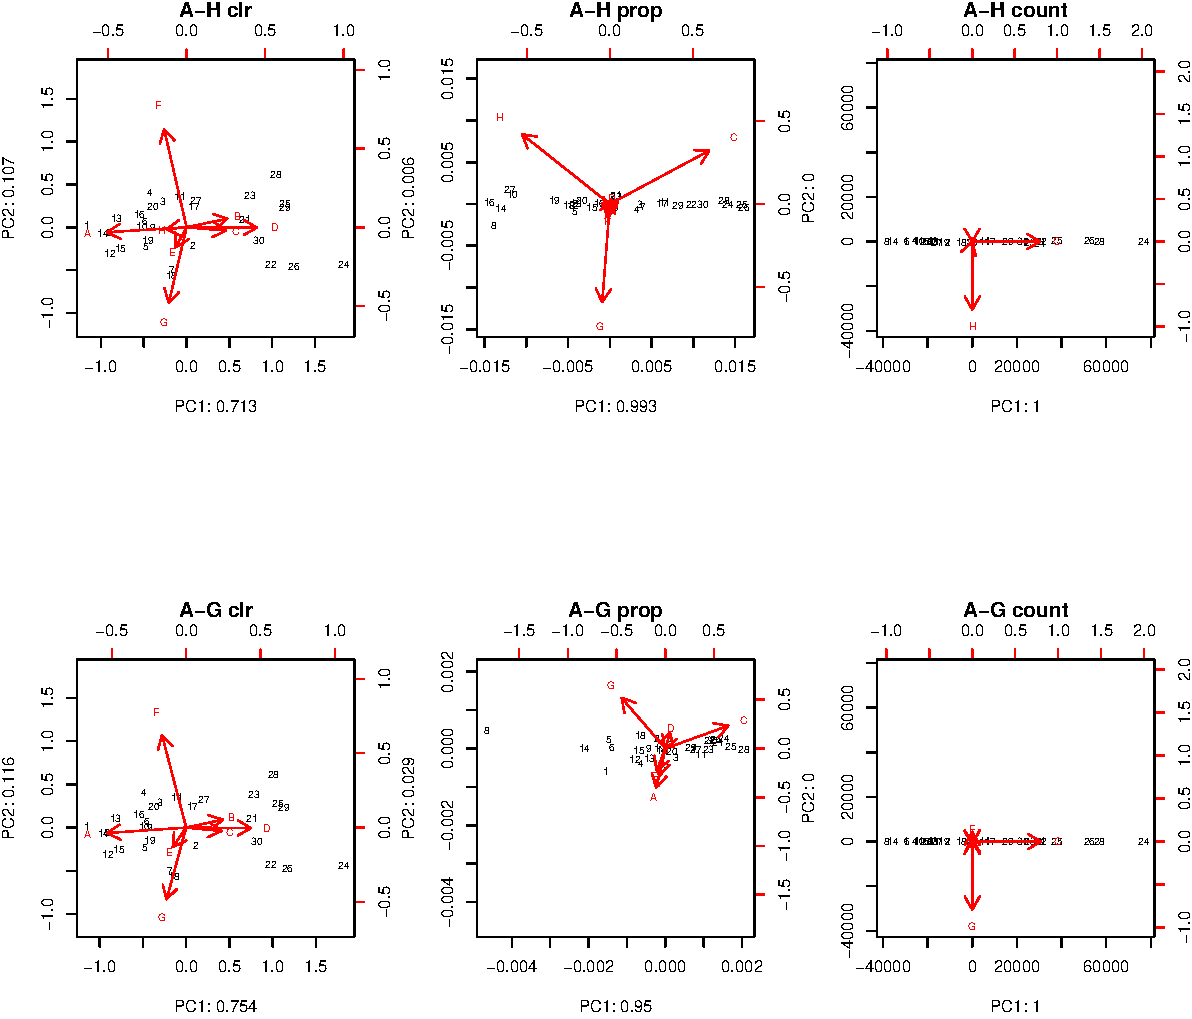
\includegraphics{_main_files/figure-latex/unnamed-chunk-1-1.pdf}
\caption{\label{fig:unnamed-chunk-1}The same plots for the supra and
subgingival plaque samples. We see that we have statistical
significance, but the biological relevance is difficult to defend
because of the very small effect sizes.}
\end{figure}

\newpage

\#References

\hypertarget{references}{%
\chapter{References}\label{references}}

\hypertarget{refs}{}
\leavevmode\hypertarget{ref-Aitchison:1986}{}%
Aitchison, J. 1986. \emph{The Statistical Analysis of Compositional
Data}. London, England: Chapman \& Hall.

\leavevmode\hypertarget{ref-aitchison:2005}{}%
Aitchison, J., and J. J. Egozcue. 2005. ``Compositional Data Analysis:
Where Are We and Where Should We Be Heading?'' \emph{Mathematical
Geology} 37 (7). Springer:829--50.

\leavevmode\hypertarget{ref-altman:1983}{}%
Altman, D. G., and J. M. Bland. 1983. ``Measurement in Medicine: The
Analysis of Method Comparison Studies.'' \emph{Journal of the Royal
Statistical Society. Series D (the Statistician)} 32 (3). Wiley for the
Royal Statistical Society:pp. 307--17.
\url{http://www.jstor.org/stable/2987937}.

\leavevmode\hypertarget{ref-Andersson:2008}{}%
Andersson, Anders F, Mathilda Lindberg, Hedvig Jakobsson, Fredrik
Bäckhed, Pål Nyrén, and Lars Engstrand. 2008. ``Comparative Analysis of
Human Gut Microbiota by Barcoded Pyrosequencing.'' \emph{PLoS One} 3
(7):e2836. \url{https://doi.org/10.1371/journal.pone.0002836}.

\leavevmode\hypertarget{ref-auer:2011}{}%
Auer, Paul L, and Rebecca W Doerge. 2011. ``A Two-Stage Poisson Model
for Testing RNA-seq Data.'' \emph{Statistical Applications in Genetics
and Molecular Biology} 10 (1).

\leavevmode\hypertarget{ref-barcelo:2001}{}%
Barceló-Vidal, Carles, Josep A Martín-Fernández, and Vera
Pawlowsky-Glahn. 2001. ``Mathematical Foundations of Compositional Data
Analysis.'' In \emph{Proceedings of IAMG}, 1:1--20.

\leavevmode\hypertarget{ref-mRNA:2002}{}%
Bernstein, Jonathan A, Arkady B Khodursky, Pei-Hsun Lin, Sue Lin-Chao,
and Stanley N Cohen. 2002. ``Global Analysis of mRNA Decay and Abundance
in Escherichia Coli at Single-Gene Resolution Using Two-Color
Fluorescent Dna Microarrays.'' \emph{Proceedings of the National Academy
of Sciences} 99 (15). National Acad Sciences:9697--9702.

\leavevmode\hypertarget{ref-bian:2017}{}%
Bian, Gaorui, Gregory B Gloor, Aihua Gong, Changsheng Jia, Wei Zhang,
Jun Hu, Hong Zhang, et al. n.d. ``The Gut Microbiota of Healthy Aged
Chinese Is Similar to That of the Healthy Young.'' \emph{mSphere} 2
(5):e00327--17. \url{https://doi.org/10.1128/mSphere.00327-17}.

\leavevmode\hypertarget{ref-box:1976}{}%
Box, George EP. 1976. ``Science and Statistics.'' \emph{Journal of the
American Statistical Association} 71 (356). Taylor \& Francis:791--99.

\leavevmode\hypertarget{ref-Colquhoun:2014aa}{}%
Colquhoun, David. 2014. ``An Investigation of the False Discovery Rate
and the Misinterpretation of P-Values.'' \emph{R Soc Open Sci} 1
(3):140216. \url{https://doi.org/10.1098/rsos.140216}.

\leavevmode\hypertarget{ref-Cui:2003aa}{}%
Cui, Xiangqin, and Gary A Churchill. 2003. ``Statistical Tests for
Differential Expression in cDNA Microarray Experiments.'' \emph{Genome
Biol} 4 (4):210.1--210.10.

\leavevmode\hypertarget{ref-Cumming:2008aa}{}%
Cumming, Geoff. 2008. ``Replication and P Intervals: P Values Predict
the Future Only Vaguely, but Confidence Intervals Do Much Better.''
\emph{Perspect Psychol Sci} 3 (4):286--300.
\url{https://doi.org/10.1111/j.1745-6924.2008.00079.x}.

\leavevmode\hypertarget{ref-Dillies:2013}{}%
Dillies, Marie-Agnès, Andrea Rau, Julie Aubert, Christelle
Hennequet-Antier, Marine Jeanmougin, Nicolas Servant, Céline Keime, et
al. 2013. ``A Comprehensive Evaluation of Normalization Methods for
Illumina High-Throughput RNA Sequencing Data Analysis.'' \emph{Brief
Bioinform} 14 (6):671--83. \url{https://doi.org/10.1093/bib/bbs046}.

\leavevmode\hypertarget{ref-egozcue2005}{}%
Egozcue, JJ, and V. Pawlowsky-Glahn. 2005. ``Groups of Parts and Their
Balances in Compositional Data Analysis.'' \emph{Mathematical Geology}
37 (7). Springer:795--828.

\leavevmode\hypertarget{ref-egozcue:AJS}{}%
Egozcue, Juan José, Vera Pawlowsky-Glahn, and Gregory B. Gloor. 2018.
``Linear Association in Compositional Data Analysis.'' \emph{Austrian
Journal of Statistics} 47 (1):3--31.

\leavevmode\hypertarget{ref-erb:2016}{}%
Erb, Ionas, and Cédric Notredame. 2016. ``How Should We Measure
Proportionality on Relative Gene Expression Data?'' \emph{Theory in
Biosciences} 135 (1):21--36.

\leavevmode\hypertarget{ref-Erb134536}{}%
Erb, Ionas, Thomas Quinn, David Lovell, and Cedric Notredame. 2017.
``Differential Proportionality - a Normalization-Free Approach to
Differential Gene Expression.'' \emph{bioRxiv}. Cold Spring Harbor
Laboratory. \url{https://doi.org/10.1101/134536}.

\leavevmode\hypertarget{ref-fernandes:2013}{}%
Fernandes, Andrew D, Jean M Macklaim, Thomas G Linn, Gregor Reid, and
Gregory B Gloor. 2013. ``ANOVA-Like Differential Expression (Aldex)
Analysis for Mixed Population Rna-Seq.'' \emph{PLoS One} 8 (7):e67019.
\url{https://doi.org/10.1371/journal.pone.0067019}.

\leavevmode\hypertarget{ref-fernandes:2014}{}%
Fernandes, Andrew D, Jennifer Ns Reid, Jean M Macklaim, Thomas A
McMurrough, David R Edgell, and Gregory B Gloor. 2014. ``Unifying the
Analysis of High-Throughput Sequencing Datasets: Characterizing RNA-Seq,
16S RRNA Gene Sequencing and Selective Growth Experiments by
Compositional Data Analysis.'' \emph{Microbiome} 2:15.1--15.13.
\url{https://doi.org/10.1186/2049-2618-2-15}.

\leavevmode\hypertarget{ref-Friedman:2012}{}%
Friedman, Jonathan, and Eric J Alm. 2012. ``Inferring Correlation
Networks from Genomic Survey Data.'' \emph{PLoS Comput Biol} 8
(9):e1002687. \url{https://doi.org/10.1371/journal.pcbi.1002687}.

\leavevmode\hypertarget{ref-forking:2013}{}%
Gelman, Andrew, and Eric Loken. n.d. ``The Garden of Forking Paths: Why
Multiple Comparisons Can Be a Problem, Even When There Is No `Fishing
Expedition' or `P-Hacking' and the Research Hypothesis Was Posited Ahead
of Time.''
\url{http://www.stat.columbia.edu/~gelman/research/unpublished/p_hacking.pdf}.

\leavevmode\hypertarget{ref-Gierlinski:2015aa}{}%
Gierliński, Marek, Christian Cole, Pietà Schofield, Nicholas J Schurch,
Alexander Sherstnev, Vijender Singh, Nicola Wrobel, et al. 2015.
``Statistical Models for Rna-Seq Data Derived from a Two-Condition
48-Replicate Experiment.'' \emph{Bioinformatics} 31 (22):3625--30.
\url{https://doi.org/10.1093/bioinformatics/btv425}.

\leavevmode\hypertarget{ref-Gloor:2015}{}%
Gloor, Gregory B., Jean M. Macklaim, and Andrew D. Fernandes. 2016.
``Displaying Variation in Large Datasets: A Visual Summary of Effect
Sizes.'' \emph{Journal of Computational and Graphical Statistics} 25
(3):971--9.

\leavevmode\hypertarget{ref-Gloor:2010}{}%
Gloor, Gregory B, Ruben Hummelen, Jean M Macklaim, Russell J Dickson,
Andrew D Fernandes, Roderick MacPhee, and Gregor Reid. 2010.
``Microbiome Profiling by Illumina Sequencing of Combinatorial
Sequence-Tagged PCR Products.'' \emph{PLoS One} 5 (10):e15406.
\url{https://doi.org/10.1371/journal.pone.0015406}.

\leavevmode\hypertarget{ref-gloorAJS:2016}{}%
Gloor, Gregory B, Jean M Macklaim, Michael Vu, and Andrew D Fernandes.
2016. ``Compositional Uncertainty Should Not Be Ignored in
High-Throughput Sequencing Data Analysis.'' \emph{Austrian Journal of
Statistics} 45:73--87. \url{https://doi.org/doi:10.17713/ajs.v45i4.122}.

\leavevmode\hypertarget{ref-Gloor:2016cjm}{}%
Gloor, Gregory B, and Gregor Reid. 2016. ``Compositional Analysis: A
Valid Approach to Analyze Microbiome High-Throughput Sequencing Data.''
\emph{Can J Microbiol} 62 (8):692--703.
\url{https://doi.org/10.1139/cjm-2015-0821}.

\leavevmode\hypertarget{ref-gloor2016s}{}%
Gloor, Gregory B, Jia Rong Wu, Vera Pawlowsky-Glahn, and Juan José
Egozcue. 2016. ``It's All Relative: Analyzing Microbiome Data as
Compositions.'' \emph{Ann Epidemiol} 26 (5):322--9.
\url{https://doi.org/10.1016/j.annepidem.2016.03.003}.

\leavevmode\hypertarget{ref-Gorzelak:2015aa}{}%
Gorzelak, Monika A, Sandeep K Gill, Nishat Tasnim, Zahra Ahmadi-Vand,
Michael Jay, and Deanna L Gibson. 2015. ``Methods for Improving Human
Gut Microbiome Data by Reducing Variability Through Sample Processing
and Storage of Stool.'' \emph{PLoS One} 10 (8):e0134802.
\url{https://doi.org/10.1371/journal.pone.0134802}.

\leavevmode\hypertarget{ref-Halsey:2015aa}{}%
Halsey, Lewis G, Douglas Curran-Everett, Sarah L Vowler, and Gordon B
Drummond. 2015. ``The Fickle P Value Generates Irreproducible Results.''
\emph{Nat Methods} 12 (3):179--85.
\url{https://doi.org/10.1038/nmeth.3288}.

\leavevmode\hypertarget{ref-hawinkel2017}{}%
Hawinkel, Stijn, Federico Mattiello, Luc Bijnens, and Olivier Thas.
2017. ``A Broken Promise: Microbiome Differential Abundance Methods Do
Not Control the False Discovery Rate.'' \emph{Briefings in
Bioinformatics}. Oxford University Press, bbx104.

\leavevmode\hypertarget{ref-Horner-Devine:2004aa}{}%
Horner-Devine, M Claire, Melissa Lage, Jennifer B Hughes, and Brendan J
M Bohannan. 2004. ``A Taxa-Area Relationship for Bacteria.''
\emph{Nature} 432 (7018):750--3.
\url{https://doi.org/10.1038/nature03073}.

\leavevmode\hypertarget{ref-Hsiao:2013}{}%
Hsiao, Elaine Y, Sara W McBride, Sophia Hsien, Gil Sharon, Embriette R
Hyde, Tyler McCue, Julian A Codelli, et al. 2013. ``Microbiota Modulate
Behavioral and Physiological Abnormalities Associated with
Neurodevelopmental Disorders.'' \emph{Cell} 155 (7):1451--63.
\url{https://doi.org/10.1016/j.cell.2013.11.024}.

\leavevmode\hypertarget{ref-Jaynes:2003}{}%
Jaynes, E. T, and G. Larry Bretthorst. 2003. \emph{Probability Theory:
The Logic of Science}. Cambridge, UK: Cambridge University Press.
\url{http://www.loc.gov/catdir/samples/cam033/2002071486.html}.

\leavevmode\hypertarget{ref-Kaul:2017aa}{}%
Kaul, Abhishek, Siddhartha Mandal, Ori Davidov, and Shyamal D Peddada.
2017. ``Analysis of Microbiome Data in the Presence of Excess Zeros.''
\emph{Front Microbiol} 8:2114.
\url{https://doi.org/10.3389/fmicb.2017.02114}.

\leavevmode\hypertarget{ref-Kurtz:2015}{}%
Kurtz, Zachary D, Christian L Müller, Emily R Miraldi, Dan R Littman,
Martin J Blaser, and Richard A Bonneau. 2015. ``Sparse and
Compositionally Robust Inference of Microbial Ecological Networks.''
\emph{PLoS Comput Biol} 11 (5):e1004226.
\url{https://doi.org/10.1371/journal.pcbi.1004226}.

\leavevmode\hypertarget{ref-Kvam:2012}{}%
Kvam, Vanessa M, Peng Liu, and Yaqing Si. 2012. ``A Comparison of
Statistical Methods for Detecting Differentially Expressed Genes from
RNA-seq Data.'' \emph{Am J Bot} 99 (2):248--56.
\url{https://doi.org/10.3732/ajb.1100340}.

\leavevmode\hypertarget{ref-Li:2010aa}{}%
Li, Bo, Victor Ruotti, Ron M Stewart, James A Thomson, and Colin N
Dewey. 2010. ``RNA-Seq Gene Expression Estimation with Read Mapping
Uncertainty.'' \emph{Bioinformatics} 26 (4):493--500.
\url{https://doi.org/10.1093/bioinformatics/btp692}.

\leavevmode\hypertarget{ref-Lovell:2015}{}%
Lovell, David, Vera Pawlowsky-Glahn, Juan José Egozcue, Samuel
Marguerat, and Jürg Bähler. 2015. ``Proportionality: A Valid Alternative
to Correlation for Relative Data.'' \emph{PLoS Comput Biol} 11
(3):e1004075. \url{https://doi.org/10.1371/journal.pcbi.1004075}.

\leavevmode\hypertarget{ref-Loven:2012aa}{}%
Lovén, Jakob, David A Orlando, Alla A Sigova, Charles Y Lin, Peter B
Rahl, Christopher B Burge, David L Levens, Tong Ihn Lee, and Richard A
Young. 2012. ``Revisiting Global Gene Expression Analysis.'' \emph{Cell}
151 (3):476--82. \url{https://doi.org/10.1016/j.cell.2012.10.012}.

\leavevmode\hypertarget{ref-unifrac:2005}{}%
Lozupone, Catherine, and Rob Knight. 2005. ``UniFrac: A New Phylogenetic
Method for Comparing Microbial Communities.'' \emph{Applied and
Environmental Microbiology} 71 (12). Am Soc Microbiol:8228--35.

\leavevmode\hypertarget{ref-Lozupone:2011aa}{}%
Lozupone, Catherine, Manuel E Lladser, Dan Knights, Jesse Stombaugh, and
Rob Knight. 2011. ``UniFrac: An Effective Distance Metric for Microbial
Community Comparison.'' \emph{ISME J} 5 (2):169--72.
\url{https://doi.org/10.1038/ismej.2010.133}.

\leavevmode\hypertarget{ref-macklaim:2013}{}%
Macklaim, M Jean, D Andrew Fernandes, M Julia Di Bella, Jo-Anne Hammond,
Gregor Reid, and Gregory B Gloor. 2013. ``Comparative Meta-RNA-Seq of
the Vaginal Microbiota and Differential Expression by
\emph{Lactobacillus Iners} in Health and Dysbiosis.'' \emph{Microbiome}
1:15.
\href{https://doi.org/doi:\%2010.1186/2049-2618-1-12}{https://doi.org/doi: 10.1186/2049-2618-1-12}.

\leavevmode\hypertarget{ref-ancom:2015}{}%
Mandal, Siddhartha, Will Van Treuren, Richard A White, Merete Eggesbø,
Rob Knight, and Shyamal D Peddada. 2015. ``Analysis of Composition of
Microbiomes: A Novel Method for Studying Microbial Composition.''
\emph{Microb Ecol Health Dis} 26:27663.

\leavevmode\hypertarget{ref-martin1998measures}{}%
Martín-Fernández, JA, C Barceló-Vidal, V Pawlowsky-Glahn, A Buccianti, G
Nardi, and R Potenza. 1998. ``Measures of Difference for Compositional
Data and Hierarchical Clustering Methods.'' In \emph{Proceedings of
IAMG}, 98:526--31.

\leavevmode\hypertarget{ref-McMurdie:2014a}{}%
McMurdie, Paul J, and Susan Holmes. 2014. ``Waste Not, Want Not: Why
Rarefying Microbiome Data Is Inadmissible.'' \emph{PLoS Comput Biol} 10
(4):e1003531. \url{https://doi.org/10.1371/journal.pcbi.1003531}.

\leavevmode\hypertarget{ref-mcmurrough:2014}{}%
McMurrough, Thomas A, Russell J Dickson, Stephanie M F Thibert, Gregory
B Gloor, and David R Edgell. 2014. ``Control of Catalytic Efficiency by
a Coevolving Network of Catalytic and Noncatalytic Residues.''
\emph{Proc Natl Acad Sci U S A} 111 (23):E2376--83.
\url{https://doi.org/10.1073/pnas.1322352111}.

\leavevmode\hypertarget{ref-Mortazavi:2008}{}%
Mortazavi, Ali, Brian A Williams, Kenneth McCue, Lorian Schaeffer, and
Barbara Wold. 2008. ``Mapping and Quantifying Mammalian Transcriptomes
by RNA-seq.'' \emph{Nat Methods} 5 (7):621--8.
\url{https://doi.org/10.1038/nmeth.1226}.

\leavevmode\hypertarget{ref-Newey:1994}{}%
Newey, Whitney K., and Daniel McFadden. 1994. ``Large Sample Estimation
and Hypothesis Testing.'' In \emph{Handbook of Econometrics}, edited by
Robert Engle and Daniel McFadden, 4:2111---2245. Elsevier Science.

\leavevmode\hypertarget{ref-vegan:2017}{}%
Oksanen, Jari, F. Guillaume Blanchet, Michael Friendly, Roeland Kindt,
Pierre Legendre, Dan McGlinn, Peter R. Minchin, et al. 2017. ``Vegan:
Community Ecology Package.'' 2017.
\url{https://CRAN.R-project.org/package=vegan}.

\leavevmode\hypertarget{ref-Pachter:2011}{}%
Pachter, Lior. 2011. ``Models for Transcript Quantiffication from
RNA-seq.'' \emph{ArXiv} 1104.3889 (v2).

\leavevmode\hypertarget{ref-Parameswaran:2007aa}{}%
Parameswaran, Poornima, Roxana Jalili, Li Tao, Shadi Shokralla, Baback
Gharizadeh, Mostafa Ronaghi, and Andrew Z Fire. 2007. ``A
Pyrosequencing-Tailored Nucleotide Barcode Design Unveils Opportunities
for Large-Scale Sample Multiplexing.'' \emph{Nucleic Acids Res} 35
(19):e130. \url{https://doi.org/10.1093/nar/gkm760}.

\leavevmode\hypertarget{ref-Paulson:2013aa}{}%
Paulson, Joseph N, O Colin Stine, Héctor Corrada Bravo, and Mihai Pop.
2013. ``Differential Abundance Analysis for Microbial Marker-Gene
Surveys.'' \emph{Nat Methods} 10 (12):1200--1202.
\url{https://doi.org/10.1038/nmeth.2658}.

\leavevmode\hypertarget{ref-Pawlowsky-Glahn:2006}{}%
Pawlowsky-Glahn, V., and J. J. Egozcue. 2006. ``Compositional Data and
Their Analysis: An Introduction.'' \emph{Geological Society, London,
Special Publications} 264 (1):1--10.
\url{https://doi.org/10.1144/GSL.SP.2006.264.01.01}.

\leavevmode\hypertarget{ref-pawlowsky2011compositional}{}%
Pawlowsky-Glahn, Vera, and Antonella Buccianti. 2011.
\emph{Compositional Data Analysis: Theory and Applications}. John Wiley
\& Sons.

\leavevmode\hypertarget{ref-pawlowsky2015modeling}{}%
Pawlowsky-Glahn, Vera, Juan José Egozcue, and Raimon Tolosana-Delgado.
2015. \emph{Modeling and Analysis of Compositional Data}. John Wiley \&
Sons.

\leavevmode\hypertarget{ref-Pearson:1896}{}%
Pearson, Karl. 1897. ``Mathematical Contributions to the Theory of
Evolution. -- on a Form of Spurious Correlation Which May Arise When
Indices Are Used in the Measurement of Organs.'' \emph{Proceedings of
the Royal Society of London} 60:489--98.

\leavevmode\hypertarget{ref-Quinn206425}{}%
Quinn, Thomas P., Ionas Erb, Mark F. Richardson, and Tamsyn M. Crowley.
2017. ``Understanding Sequencing Data as Compositions: An Outlook and
Review.'' \emph{bioRxiv}. Cold Spring Harbor Laboratory.
\url{https://doi.org/10.1101/206425}.

\leavevmode\hypertarget{ref-Quinn:2017}{}%
Quinn, Thomas, Mark F Richardson, David Lovell, and Tamsyn Crowley.
2017. ``Propr: An R-Package for Identifying Proportionally Abundant
Features Using Compositional Data Analysis.'' \emph{bioRxiv}. Cold
Spring Harbor Labs Journals. \url{https://doi.org/10.1101/104935}.

\leavevmode\hypertarget{ref-Robinson:2010}{}%
Robinson, Mark D, Davis J McCarthy, and Gordon K Smyth. 2010. ``EdgeR: A
Bioconductor Package for Differential Expression Analysis of Digital
Gene Expression Data.'' \emph{Bioinformatics} 26 (1):139--40.
\url{https://doi.org/10.1093/bioinformatics/btp616}.

\leavevmode\hypertarget{ref-Robinson:2010a}{}%
Robinson, Mark D, and Alicia Oshlack. 2010. ``A Scaling Normalization
Method for Differential Expression Analysis of RNA-seq Data.''
\emph{Genome Biol} 11 (3):R25.1--R25.9.
\url{https://doi.org/10.1186/gb-2010-11-3-r25}.

\leavevmode\hypertarget{ref-Silverman:2017aa}{}%
Silverman, Justin D, Alex D Washburne, Sayan Mukherjee, and Lawrence A
David. 2017. ``A Phylogenetic Transform Enhances Analysis of
Compositional Microbiota Data.'' \emph{Elife} 6 (February):21887.
\url{https://doi.org/10.7554/eLife.21887}.

\leavevmode\hypertarget{ref-Taniguchi:2010aa}{}%
Taniguchi, Yuichi, Paul J Choi, Gene-Wei Li, Huiyi Chen, Mohan Babu,
Jeremy Hearn, Andrew Emili, and X Sunney Xie. 2010. ``Quantifying E.
Coli Proteome and Transcriptome with Single-Molecule Sensitivity in
Single Cells.'' \emph{Science} 329 (5991):533--8.
\url{https://doi.org/10.1126/science.1188308}.

\leavevmode\hypertarget{ref-Thorsen:2016aa}{}%
Thorsen, Jonathan, Asker Brejnrod, Martin Mortensen, Morten A Rasmussen,
Jakob Stokholm, Waleed Abu Al-Soud, Søren Sørensen, Hans Bisgaard, and
Johannes Waage. 2016. ``Large-Scale Benchmarking Reveals False
Discoveries and Count Transformation Sensitivity in 16S RRNA Gene
Amplicon Data Analysis Methods Used in Microbiome Studies.''
\emph{Microbiome} 4 (1):62.
\url{https://doi.org/10.1186/s40168-016-0208-8}.

\leavevmode\hypertarget{ref-Tsilimigras:2016aa}{}%
Tsilimigras, Matthew C B, and Anthony A Fodor. 2016. ``Compositional
Data Analysis of the Microbiome: Fundamentals, Tools, and Challenges.''
\emph{Ann Epidemiol} 26 (5):330--5.
\url{https://doi.org/10.1016/j.annepidem.2016.03.002}.

\leavevmode\hypertarget{ref-van2013}{}%
Van den Boogaart, K Gerald, and Raimon Tolosana-Delgado. 2013.
\emph{Analyzing Compositional Data with R}. Springer, London, UK.

\leavevmode\hypertarget{ref-Vandesompele:2002aa}{}%
Vandesompele, Jo, Katleen De Preter, Filip Pattyn, Bruce Poppe, Nadine
Van Roy, Anne De Paepe, and Frank Speleman. 2002. ``Accurate
Normalization of Real-Time Quantitative Rt-Pcr Data by Geometric
Averaging of Multiple Internal Control Genes.'' \emph{Genome Biol} 3
(7):RESEARCH0034.

\leavevmode\hypertarget{ref-Warton:2011aa}{}%
Warton, David I, and Francis K C Hui. 2011. ``The Arcsine Is Asinine:
The Analysis of Proportions in Ecology.'' \emph{Ecology} 92 (1):3--10.

\leavevmode\hypertarget{ref-Washburne:2017aa}{}%
Washburne, Alex D, Justin D Silverman, Jonathan W Leff, Dominic J
Bennett, John L Darcy, Sayan Mukherjee, Noah Fierer, and Lawrence A
David. 2017. ``Phylogenetic Factorization of Compositional Data Yields
Lineage-Level Associations in Microbiome Datasets.'' \emph{PeerJ}
5:e2969. \url{https://doi.org/10.7717/peerj.2969}.

\leavevmode\hypertarget{ref-Weiss:2017aa}{}%
Weiss, Sophie, Zhenjiang Zech Xu, Shyamal Peddada, Amnon Amir, Kyle
Bittinger, Antonio Gonzalez, Catherine Lozupone, et al. 2017.
``Normalization and Microbial Differential Abundance Strategies Depend
Upon Data Characteristics.'' \emph{Microbiome} 5 (1):27.
\url{https://doi.org/10.1186/s40168-017-0237-y}.

\leavevmode\hypertarget{ref-White:2009}{}%
White, James Robert, Niranjan Nagarajan, and Mihai Pop. 2009.
``Statistical Methods for Detecting Differentially Abundant Features in
Clinical Metagenomic Samples.'' \emph{PLoS Comput Biol} 5 (4):e1000352.
\url{https://doi.org/10.1371/journal.pcbi.1000352}.

\leavevmode\hypertarget{ref-Wolfs:2016aa}{}%
Wolfs, Jason M, Thomas A Hamilton, Jeremy T Lant, Marcon Laforet, Jenny
Zhang, Louisa M Salemi, Gregory B Gloor, Caroline Schild-Poulter, and
David R Edgell. 2016. ``Biasing Genome-Editing Events Toward Precise
Length Deletions with an Rna-Guided Tevcas9 Dual Nuclease.'' \emph{Proc
Natl Acad Sci U S A}, December.
\url{https://doi.org/10.1073/pnas.1616343114}.

\leavevmode\hypertarget{ref-Wong:2016aa}{}%
Wong, Ruth G, Jia R Wu, and Gregory B Gloor. 2016. ``Expanding the
UniFrac Toolbox.'' \emph{PLoS One} 11 (9):e0161196.
\url{https://doi.org/10.1371/journal.pone.0161196}.

\leavevmode\hypertarget{ref-Zozaya:2010}{}%
Zozaya-Hinchliffe, Marcela, Rebecca Lillis, David H Martin, and Michael
J Ferris. 2010. ``Quantitative Pcr Assessments of Bacterial Species in
Women with and Without Bacterial Vaginosis.'' \emph{J Clin Microbiol} 48
(5):1812--9. \url{https://doi.org/10.1128/JCM.00851-09}.


\end{document}
